\documentclass[a4paper,12pt]{article}

\usepackage[style=authoryear,backend=bibtex,sorting=nyt,maxcitenames=2,maxbibnames=99]{biblatex}
\addbibresource{reference.bib}

\newcommand{\HRule}{\rule{\linewidth}{0.5mm}}
\newcommand{\Hrule}{\rule{\linewidth}{0.3mm}}
\usepackage[left=2cm,right=2cm,top=2cm,bottom=2cm]{geometry}

\usepackage{Mydef}
\emergencystretch=2.5em


\newcommand{\stitle}{Paper Reading}
\newcommand{\name}{Zhan Zhiyuan}
\begin{document}
\begin{center}
  \Large \textbf{Stochastic Analysis}
\end{center}
\begin{center}\vspace{0.2em} {\Large \name\\}
  \end{center}

\section{Review: Probability and Stochastic}

Let $(\Omega, \mathcal{F}, \Pb)$ be a probability space. Let $\mathcal{R}^d$ be the Borel sets of $\R^d$.
\begin{itemize}
  \item Independence: First, a collection of $\sigma$-algebras $(\mathcal{F}_{\lambda})_{\lambda \in \Lambda}$ is called independent if for any $k \in \N$ and any $i_1,i_2,\cdots,i_k \in \Lambda$,
  \begin{equation*}
    \Pb(C_1\cap C_2 \cap\cdots\cap C_k) = \prod_{j=1}^k\Pb(C_j),~\forall~C_j \in \mathcal{F}_{i_j}
  \end{equation*}
  And for a collection of random variables $(X_{\lambda})_{\lambda \in \Lambda}$, each
  \begin{equation*}
    \sigma(X_{\lambda}) \defeq \bb{X_{\lambda}^{-1}(A) \colon A \in \mathcal{R}}
  \end{equation*}
  is a $\sigma$-algebra. So $(X_{\lambda})_{\lambda \in \Lambda}$ is said independent if the corresponding $\bc{\sigma(X_{\lambda})}_{\lambda \in \Lambda}$ is independent.

  \begin{thm}
    For independent $(\mathcal{F}_{\lambda})_{\lambda \in \Lambda}$ and $N \in \N \cup \bb{\infty}$, let $\Lambda_n \subset \Lambda$ for $n = 1,2, \cdots,N$ be disjoint, then
    \begin{equation*}
      \bc{\sigma\bc{\bigcup_{\lambda \in \Lambda_n}\mathcal{F}_{\lambda}}}_{n=1}^N
    \end{equation*}
    is independent.
  \end{thm}

  \item Convergence of random variables: Let $\bb{X_n}_{n\in \N}$ be a sequence of random variables.
  \begin{enumerate}[label=(\arabic*)]
    \item $X_n\xrightarrow{a.e}X$ almost everywhere if $\Pb\bc{\bb{\omega \in \Omega \colon \lim_{n}X_n(\omega) = X(\omega)}} = 1$.

    \item $X_n\xrightarrow{\Pb}X$ in probability if 
    \begin{equation*}
      \forall~\varepsilon>0,~\lim_{n}\Pb\bc{\bb{\omega \in \Omega \colon \abs{X_n(\omega) -X(\omega)} > \varepsilon}} = 0
    \end{equation*}
    In particular, if $X_n\xrightarrow{\Pb} 0$, then $X_n = o_{p}(1)$.
    \begin{rmk}
      $X_n$ is said tight denoted by $X_n = \mathcal{O}_p(1)$ if 
      \begin{equation*}
        \forall~\varepsilon > 0,~\exists~M>0,~s.t.~\sup_n \Pb\bc{\bb{\omega \in \Omega \colon \abs{X_n(\omega)} > M}} < \varepsilon
      \end{equation*}
    \end{rmk}

    \item For $\alpha > 0$, let $X_n \in L^{\alpha}(\Omega, \Pb)$. $X_n \rightarrow X$ in $\alpha$-mean if $\lim_n\E[\abs{X_n - X}^{\alpha}] = 0$.
  \end{enumerate}
  \begin{thm}
    For the convergence of $X_n$,
    \begin{enumerate}[label=(\arabic*)]
      \item $X_n\xrightarrow{a.e}X$ implies $X_n\xrightarrow{\Pb}X$;
      \item $X_n \rightarrow X$ in $\alpha$-mean implies $X_n\xrightarrow{\Pb}X$.
    \end{enumerate}
  \end{thm}
  \begin{thm}[Strong Law of Large Number]
    Let $\bb{X_n}_{n=1}^{\infty}$ be \emph{i.i.d} random variables and $X_1 \in L^1$. Then
    \begin{equation*}
      \frac{X_1 + X_2 + \cdots + X_n}{n} \xrightarrow{a.e.} \E[X_1]
    \end{equation*}
  \end{thm}

  \item Convergence in distribution: Let $\bb{X_n}$ be a sequence of $\R^k$-valued random variables with distribution functions $F_n(x)$ and $X $ be a $\R^k$-valued random variable with distribution functions $F(x)$. $X_n \xrightarrow{d}X$ in distribution if for any continuous point $x$ of $F(x)$
  \begin{equation*}
    \lim_{n\sto \infty} F_n(x) = F(x)
  \end{equation*}
  \begin{rmk}
    Note that it does not require $X_n$ and $X$ are in the same probability space. In fact, convergence in distribution is equivalent to the weak convergence of $\Pb_n \sto \Pb$ when considering the metric space.
  \end{rmk}
  \begin{thm}
    The following statements are equivalent.
    \begin{enumerate}[label=(\arabic*)]
      \item $X_d \xrightarrow{d}X$ $\R^k$-valued random variables.
      \item For all $f \in \mathcal{C}_b(\R^k)$, $\E[f(X_n)] \sto \E[f(X)]$.
      \item For all $f \in \mathcal{C}_b(\R^k)$ uniformly continuous, $\E[f(X_n)] \sto \E[f(X)]$.
      \item For any closed $A \in \R^k$, 
      \begin{equation*}
        \limsup_n \Pb_n(A) \leqslant \Pb(A)
      \end{equation*}
      \item For any open $A \in \R^k$, 
      \begin{equation*}
        \liminf_n \Pb_n(A) \geqslant \Pb(A)
      \end{equation*}
    \end{enumerate}
  \end{thm}
  \begin{thm}
    Let $\bb{X_n}_{n\in \N}$ and $X$ be $\R^k$-valued random variables.
    \begin{enumerate}[label=(\arabic*)]
      \item If $X_d \xrightarrow{d}X$, then for any $g \in \mathcal{C}(\R^k, \R^m)$, $g(X_k) \xrightarrow{d} g(X)$.
      \item $X_d \xrightarrow{\Pb}X$ implies $X_d \xrightarrow{d}X$.
    \end{enumerate}
  \end{thm}
  By the characteristic function $\phi_X(\lambda) = \E[e^{i\lambda X}]$, it can prove the following central limit theorem.
  \begin{thm}[Central Limit Theorem]
    Let $\bb{X_n}_{n=1}^{\infty}$ be \emph{i.i.d} with mean $\mu$ and variance $\sigma^2$. Let $S_n = X_1 + X_2 + \cdots + X_n$. Then
    \begin{equation*}
      \frac{\sqrt{n}}{\sigma}(\frac{S_n}{n}-\mu) \xrightarrow{d} \mathcal{N}(0,1)
    \end{equation*}
  \end{thm}

  \item Conditional Expectation: Let $X$ be a random variable and $X \in L^1$. For $B \in \mathcal{F}$ with $\Pb(B) > 0$, let
    \begin{equation*}
      \E[X \mid B] \defeq \frac{\E[X,B]}{\Pb(B)}
    \end{equation*}
    where $\E[X,B] = \E[X\mathds{1}_B]$.
  \begin{enumerate}[label=(\arabic*)]
    \item For $\bb{B_i}_{i=1}^n \subset \mathcal{F}$ disjoint and $\Omega = \bigcup_iB_i$, define a random variable
    \begin{equation*}
      \E[X \mid \bb{B_i}](\omega) = \sum_{i=1}^n\E[X \mid B_i]\mathds{1}_{B_i}(\omega)
    \end{equation*}

    \item Let $\mathcal{B} = \sigma(B_1,B_2,\cdots,B_n)$ be the $\sigma$-algebra generated by $\bb{B_i}_{i=1}^n$. We denote
    \begin{equation*}
      \E[X \mid \bb{B_i}] = \E[X \mid \mathcal{B}]
    \end{equation*}
  \end{enumerate}
  Then we have $\E[X \mid \mathcal{B}]$ is $\mathcal{B}$-measurable and $\E\bj{\E[X \mid \mathcal{B}], B} = \E[X, B]$ for any $B \in \mathcal{B}$.
  \begin{defn}[Conditional Expectations]
    Let $X \in L^1$ and $\mathcal{G} \subset \mathcal{F}$ be a $\sigma$-subalgebra. The conditional expectation of $X$ over $\mathcal{G}$ is a random variable $Y$ such that
    \begin{enumerate}[label=(\arabic*)]
      \item $Y \in L^1$;
      \item $Y$ is $\mathcal{G}$-measurable;
      \item for any $A \in \mathcal{G}$, $\E[Y, A] = \E[X, A]$.
    \end{enumerate}
    Denote $Y = \E[X\mid \mathcal{G}]$. In particular, if $X=\mathds{1}_A$, then $\Pb(A \mid \mathcal{G}) \defeq \E[\mathds{1}_A\mid \mathcal{G}]$.
  \end{defn}
  For any $X \in L^1$ and $\sigma$-subalgebra $\mathcal{G}$, by the Radon-Nikodym theorem, $\E[X\mid \mathcal{G}]$ uniquely exists.
  \begin{thm}
    Let $X,Y \in L^1$ and $\mathcal{G}$ be a $\sigma$-subalgebra.
    \begin{enumerate}[label=(\arabic*)]
      \item For any $a,b \in \R$, $\E[aX+bY\mid \mathcal{G}] = a\E[X\mid \mathcal{G}]+b\E[Y\mid \mathcal{G}]$.
      \item $X \geqslant Y$ implies $\E[X\mid \mathcal{G}] \geqslant \E[Y\mid \mathcal{G}]$.
      \item If $X \in L^p ~(p\geqslant 1)$, then $\E[X\mid \mathcal{G}] \in L^p$ and 
      \begin{equation*}
        \norm{\E[X\mid \mathcal{G}]}_{L^p} \leqslant \norm{X}_{L^p}
      \end{equation*}
      In particular, $\abs{\E[X\mid \mathcal{G}]} \leqslant \E[\abs{X}\mid \mathcal{G}]$.
      \item For $0 \leqslant X_1 \leqslant X_2\leqslant \cdots$ random variables
      \begin{equation*}
        X_n \xrightarrow{a.e} X\quad \Rightarrow \quad \E[X_n\mid \mathcal{G}] \xrightarrow{a.e.} \E[X\mid \mathcal{G}]
      \end{equation*}
      And also $\E[\cdot \mid \mathcal{G}]$ satisfies the DCT and Fatou's lemma.
      \item If $Y$ is $\mathcal{G}$-measurable, then $\E[YX\mid \mathcal{G}] = Y\E[X\mid \mathcal{G}]$. In particular, $\E[Y\mid \mathcal{G}] = Y$.
      \item If $\mathcal{G}^{\prime}$ is also a $\sigma$-subalgebra $\mathcal{G}$, then
      \begin{equation*}
        \E[\E[X\mid \mathcal{G}] \mid \mathcal{G}^{\prime}] = \E[X \mid \mathcal{G}^{\prime}]
      \end{equation*}
      \item If $\mathcal{H}$ is independent with $\sigma(X,\mathcal{G})$, then
      \begin{equation*}
        \E[X \mid \sigma(\mathcal{G},\mathcal{H})] = \E[X \mid \sigma(\mathcal{G})]
      \end{equation*}
      In particular, if $\sigma(X)$ is independent with $\mathcal{G}$, then $\E[X\mid \mathcal{G}] = \E[X]$ \emph{a.e.}.
      \item If $\phi\colon \R \sto \R$ is convex and $\phi(X) \in L^1$, then $\phi(\E[X\mid \mathcal{G}]) \leqslant \E[\phi(X)\mid \mathcal{G}]$.
      \item If $X \in L^2$, then $Y^* = \E[X\mid \mathcal{G}]$ minimizes $\E[(X - Y)^2]$ over all $\mathcal{G}$-measurable $Y$.
    \end{enumerate}
  \end{thm}
  \begin{lem}
    Let $X,Y \colon \Omega \sto \R$ two random variables. Then it can prove that $X$ is $\sigma(Y)$-measurable if and only if there is a measurable function $g \colon \R \sto \R$ such that $X = g(Y)$.
  \end{lem}
  \begin{proof}
    It's clear that $X = g(Y)$ implies $X$ is $\sigma(Y)$-measurable. In converse, for fixed $n$, let
    \begin{equation*}
      A_{m,n} \defeq \bb{\omega \colon m2^{-n} \leqslant X(\omega) \leqslant (m+1)2^{-n}},~\forall~m\in \Z
    \end{equation*} 
    Since $X$ is $\sigma(Y)$-measurable, $A_{m,n} \in \sigma(Y)$. Therefore, there is a $B_{m,n} \in \mathcal{R}$ such that $A_{m,n} = X^{-1}(B_{m,n})$. Let
    \begin{equation*}
      g_n(x) = \sum_m m2^{-n}\mathds{1}_{B_{m,n}}(x)
    \end{equation*}
    First, for any $x$, $g_n(x)$ is monotonically increasing so $g(x) = \lim_ng_n(x)$. Second,
    \begin{equation*}
      f_n(X) \leqslant Y \leqslant f_n(X) + \frac{1}{2^n}
    \end{equation*}
    Therefore, $Y = f(X)$ by taking limits.
  \end{proof}
  \begin{rmk}
    This result is also true for multidimensional case, that is, if $Z$ is $\sigma(X,Y)$-measurable, then there is a $g \colon \R^2 \sto \R$ such that $Z = g(X,Y)$.
  \end{rmk}
  Therefore, if $\mathcal{G} = \sigma(Y)$, then $\E[X \mid Y] \defeq \E[X \mid \sigma(Y)] = g(Y)$ for some $g$.

  \begin{lem}\label{lem1}
    Let $X$ and $Y$ be two random variables on a probability space Let $(\Omega, \mathcal{F}, \mathbb{P})$ and $\mathcal{G}$ is a $\sigma$-subalgebra of $\mathcal{F}$. If $X$ is $\mathcal{G}$-measurable and $Y$ is independent with $\mathcal{G}$, then for any Borel measurable function $g \colon \mathbb{R}^2 \rightarrow \mathbb{R}$,
    \begin{equation*}
      \mathbb{E}[g(X,Y) \mid \mathcal{G}] = \mathbb{E}[g(X,Y) \mid \sigma(X)]
    \end{equation*}
  \end{lem}

  \item Stochastic Process: Let $(S,\beta_S)$ be a measurable space and $T =\R_+$ or $\Z_+$. If for any $t \in T$, $X_t \colon \Omega \sto S$ is measurable, then $X=(X_t)_{t \in T}$ is called a $S$-values stochastic process. And for any $\omega \in \Omega$, $X_{\cdot}(\omega) \colon T \sto S$, \emph{i.e.} $(X_t(\omega))_{t \in T}$ is called a sample path.

  \noindent Considering a map $p \colon S \times \beta_S \sto [0,1]$ such that
  \begin{enumerate}[label=(\arabic*)]
    \item fix any $A \in \beta_S$, $x \mapsto p(x, A)$ is measurable;
    \item fix any $x \in S$, $p(x, \cdot)$ is a probability measure defined on $S$,
  \end{enumerate}
  then $p$ is called a transition probability.

  \item Markov chain: Let $T = \Z_+$. For discrete states case, let $S = \Z$. A stochastic process $(X_t)_{t \in T}$ is called a Markov chain if for any $t \in \Z_+$, for any $x_0,x_1,\cdots,x_{t-1} \in S$ and any $A \in \beta_S$,
  \begin{enumerate}[label=(\arabic*)]
    \item $\Pb(X_0 = x_0, X_1=x_1,\cdots,X_{t-1}=x_{t-1}) > 0$;
    \item $\Pb(X_t \in A \mid X_0 = x_0, X_1=x_1,\cdots,X_{t-1}=x_{t-1}) = p(x_{t-1},A)$
  \end{enumerate}
  where $p$ is a transition probability. Then $(X_t)_{t\in T}$ is called a Markov chain.
  \begin{rmk}
    If $S = \R$, let $\sigma(X_0,X_1,\cdots,X_{t-1}) = \sigma(\sigma(X_0),\sigma(X_1),\cdots,\sigma(X_{t-1}))$,
    \begin{equation*}
      \Pb(X_t \in A \mid \sigma(X_0,X_1,\cdots,X_{t-1})) = \Pb(X_t \in A \mid \sigma(X_{t-1}))
    \end{equation*}
    then $(X_t)_{t\in T}$ is called a Markov chain.

  Note that $\Pb(X_t \in A \mid \sigma(X_0,X_1,\cdots,X_{t-1})) \eqdef \Pb(X_t \in A \mid X_0,X_1,\cdots,X_{t-1})$
  \end{rmk}
  \begin{prop}
    Let $(X_t)_{t\in T}$ be a Markov chain.
    \begin{enumerate}[label=(\arabic*)]
      \item For $Y$ nonnegative $\sigma(X_t)$-measurable, $\E[Y \mid X_0,\cdots,X_{t-1}] = \E[Y \mid X_{t-1}]$.
      \item If $n\in \N$ and $m\in \N_+$, $\Pb(X_{n+m} \in A \mid X_0,X_1,\cdots,X_{n})=\Pb(X_{n+m} \in A \mid X_{n})$.
    \end{enumerate}
  \end{prop}

  \noindent Let $S = \Z$ and $T=\Z_+$. Note if $\Pb(X_0 = x) =1$, we denote $(X_t)_{t \in T}$ by $(X_t^x)_{t \in T}$. And we denote $p(x, \bb{y}) = p(x,y)$. So $\Pb(X_1^x = y) = p(x,y)$. Moreover,
  \begin{equation*}
    \begin{split}
      \Pb(X_n^x = y) &= \sum_{x_1,\cdots,x_{n-1}}\Pb(X_1^x = x_1,\cdots,X_{n-1}^x=x_{n-1},X_n^{x}=y) \\
      &= \sum_{x_1,\cdots,x_{n-1}} p(x,x_1)p(x_1,x_2)\cdots p(x_{n-1},y) \\
      &\eqdef p^{(n)}(x,y)
    \end{split}
  \end{equation*}
  From this denotation, $p^{(n+m)}(x,y) = \sum_{x_m}p^{(n)}(x,x_m)p^{(m)}(x_m,y)$. Moreover, for $x,y \in S$, $x\rightarrow y$ means there is a $n\in \N$ such that $p^{(n)}(x,y) > 0$. And if for any $x, y\in S$, $x \leftrightarrow y$, then the Markov chain is irreducible.

  \noindent For $x \in S$, if 
  \begin{equation*}
    \Pb\bc{\bigcup_{n=1}^{\infty}X_n^x=x} = 1
  \end{equation*}
  then $x \in S$ is called recurrent. Moreover, let
  \begin{equation*}
    \begin{split}
      \tau_y^x &\defeq \inf\bb{n \geqslant 1 \colon X_n^x = y} \\
      N_y^x &\defeq \sum_{n=1}^{\infty}\mathds{1}_{\bb{X_n^x = y}}
    \end{split}
  \end{equation*}
  \begin{rmk}
    Let $\tau_x^{(k)} = \inf\bb{N \geqslant 1 \colon \sum_{j=1}^N \mathds{1}_{\bb{X_j^x = x}} \geqslant k}$ and $t_k = \tau_x^{(k)} -\tau_x^{(k-1)}$. And the Markov property guarantees $\bb{t_k}_{k=1}^{\infty}$ is independent.
  \end{rmk}
  So $x$ is recurrent $\Leftrightarrow$ $\Pb(N_x^x = \infty) = 1$ $\Leftrightarrow$ $\sum_{n=1}^{\infty}p^{(n)}(x,x) =\infty$, where the first equivalence is because
  \begin{equation*}
    \Pb(N_x^x \geqslant n) = \Pb(\tau_x^{(n)} < \infty) = \Pb(t_1 < \infty)^n = \Pb(\tau_x^x < \infty)^n
  \end{equation*}
  and the second equivalence is because
  \begin{equation*}
    \sum_{n=1}^{\infty}p^{(n)}(x,x) = \E[N_x^x] = \E[\sum_{k=1}^{\infty}\mathds{1}_{\bb{N_x^x \geqslant k}}] = \sum_{k=1}^{\infty}\Pb(\tau_x^x < \infty)^k
  \end{equation*}
  Moreover, if $x\leftrightarrow y$, then the recurrence of $x$ implies the recurrence of $y$.

  \noindent The average recurrent time of a state $x$ is defined as
  \begin{equation*}
    m(x) = \sum_{n=1}^{\infty}n\Pb(\tau_x^x=n),~\text{if } \Pb(\tau_x^x < \infty) = 1
  \end{equation*}
  otherwise, $m(x) = \infty$. Then $x$ is called positively recurrence if $m(x) < \infty$ and $x$ is called zero recurrence if $x$ is recurrent but $m(x) = \infty$. And for $x, y \in S$, 
  \begin{equation*}
    \lim_n \frac{1}{n}\sum_{l=1}^n p^{(l)}(x,y) = \frac{\Pb(\tau^x_y < \infty)}{m(y)}
  \end{equation*}

  \noindent Let $\pi$ be a distribution on $S$. If
  \begin{equation*}
    \pi(y) = \sum_{x\in S}\pi(x)p(x,y),~\forall~y\in S
  \end{equation*}
  then $\pi$ is called a stationary distribution. Moreover, for a distribution $\pi_0$ defined on $S$, let 
  \begin{equation*}
    \pi_n(y) = \sum_{x \in S}\pi_0(x)p^{(n)}(x,y)
  \end{equation*}
  Note that $\pi_n(y) = \sum_{z \in S}\pi_{n-1}(z)p(z,y)$. If there is a $\pi$ on $S$ such that for any $\pi_0$
  \begin{equation*}
    \lim_{n}\pi_n(x) = \pi(x)
  \end{equation*}
  such $\pi$ is called a limit distribution, which is also stationary.

  \begin{thm}
    For an irreducible Markov chain, TFAE
    \begin{enumerate}[label=(\arabic*)]
      \item There is a positively recurrent $x$.
      \item All $x$ is positively recurrent.
      \item There is a unique stationary distribution $\pi$ and
      \begin{equation*}
        \pi(x) = \lim_n \frac{1}{n}\sum_{l=1}^n p^{(l)}(x,x) = \frac{1}{m(x)}
      \end{equation*}
    \end{enumerate}
  \end{thm}

  \begin{thm}
    The Markov chain is irreducible.
    \begin{enumerate}[label=(\arabic*)]
      \item If there is a stationary distribution $\pi$ with $\pi(y) > 0$, then all states are recurrent.
      \item If $y$ is recurrent, then $\Pb(\tau_y^x < \infty) = 1$ for any $x \in S$.
    \end{enumerate}
  \end{thm}

  \item Poisson Random Measure: Let $\mu$ be a $\sigma$-finite measure defined on $(\R^d,\mathcal{R}^d)$. And for $E \in \R^d$ with $\mu(E) > 0$, let $\nu_E(A) \defeq \mu(A \cap E) / \mu(E)$ for any $A \in \mathcal{R}^d$ is a probability measure.

  \noindent The Poisson random measure is a family of random variables $X=(X(A))_{A \in \mathcal{R}^d}$ (or $X \colon \mathcal{R}^d \times \Omega \sto \R$) such that
  \begin{enumerate}[label=(\arabic*)]
    \item For \emph{a.e.} $\omega \in \Omega$, $X(\cdot, \omega)$ is a $\sigma$-finite measure on $\R^d$;
    \item For any $E \in \R^d$, $X(E)$ is a random variable obeying the Poisson distribution with mean $\mu(E)$;
    \item For disjoint $E_1,E_2,\cdots,E_n \in \R^d$, $X(E_1),X(E_2),\cdots,X(E_n)$ are independent.
  \end{enumerate}
  
  \noindent Existence of $X=(X(A))_{A \in \mathcal{R}^d}$. First, let $\bb{S_n}_{n=1}^{\infty} \subset \mathcal{R}^d$ be disjoint partition of $\R^d$ such that $\mu(S_n) < \infty$.
  \begin{enumerate}[label=\Roman*.]
    \item For any $n$, let $X(S_n) \sim P_o(\mu(S_n))$. And $\bb{X(S_n)}_n$ is independent.
    \item Fix $S_n$, let $\bb{E_j}_{j=1}^{\infty}$ be a disjoint partition of $S_n$. For any $k = \sum_{j=1}^mk_j$,
    \begin{equation*}
      \Pb(X(E_1)=k_1,\cdots,X(E_m)=k_m \mid X(S_n)=k) \defeq \frac{k!}{k_1!k_2!\cdots k_m!}\prod_{j=1}^m\bc{\frac{\mu(E_j)}{\mu(S_n)}}^{k_j}
    \end{equation*}
    Based on this, it is not hard to see
    \begin{equation*}
      \Pb(X(E_1)=k_1,\cdots,X(E_m)=k_m) = \prod_{j=1}^me^{-\mu(E_j)}\frac{\mu(E_j)^{k_j}}{k_j!}
    \end{equation*}
    So $X(E_j) \sim P_o(\mu(E_j))$ and they are independent. Therefore, for any $A \in \mathcal{R}^d$ and $A \in S_n$, then $\bb{A,A^c}$ is a partition so that 
    \begin{equation*}
      \Pb(X(A) = k_1 \mid X(S_n) = k) = \binom{k}{k_1}p^{k_1}(1-p)^{1-k_1}\quad \Rightarrow \quad \Pb(X(A) = k_1) = e^{-p}\frac{p^{k_1}}{k_1!}
    \end{equation*}
    where $p = \mu(A) / \mu(S_n)$. 

    \noindent Or equivalently let $N \sim P_o(\mu(S_n))$ and $\bb{X_j}_{j=1}^{\infty}$ independent with $\Pb(X_j \in A) = \mu(A) / \mu(S_n)$ for any $A \subset S_n$. Then define
    \begin{equation*}
      X(A) \defeq \sum_{j=1}^N\mathds{1}_{A}(X_j),~\forall~A\subset S_n
    \end{equation*}

    \item Finally, for any $A \in \mathcal{R}^d$,
    \begin{equation*}
      X(A) \defeq \sum_{n=1}^{\infty}X(A \cap S_n)
    \end{equation*}
  \end{enumerate}

  \item Poisson Process: Let $Y=(Y(A))_{A \in \mathcal{R}}$ be a Poisson random measure defined on $(\R, \mathcal{R}, \mu)$. Define
  \begin{equation*}
    X_t(\omega) \defeq Y([0,t])(\omega),~\forall~t\geqslant 0
  \end{equation*}
  Then $X= (X_t)_{t\geqslant 0}$ is called a Poisson process. In particular, if $\mu([a,b]) = \lambda (b-a)$, then $X$ is called a Poisson process with intensity $\lambda$.

  \begin{thm}
    Let $X$ be a Poisson process with intensity $\lambda$.
    \begin{enumerate}[label=(\arabic*)]
      \item $X_0 = 0$ \emph{a.e.}
      \item For any $0\leqslant t_0 < t_1 < t_2 < \cdots < t_n$,
      \begin{equation*}
        X_{t_1}-X_{t_0},X_{t_2}-X_{t_1},\cdots,X_{t_n}-X_{t_{n-1}}
      \end{equation*}
      are independent (such property is called independent increments).
      \item For $t > s$, $X_t - X_s \sim P_o(\lambda(t-s))$.
      \item For almost every $\omega \in \Omega$, $t \mapsto X_t(\omega)$ is right continuous, monotonously increasing and has the left limit.
    \end{enumerate}
  \end{thm}
  \begin{rmk}
    If a stochastic process $X=(X_t)_{t \geqslant 0}$ just satisfies $(4)$ except for monotonously increasing, it is called c\`adl\`ag or RCLL. If a stochastic process $X=(X_t)_{t \geqslant 0}$ satisfies $(1)(2)$ and $(4)$ except for monotonously increasing and two more properties: $X_t - X_s$ has the same distribution as $X_{t-s}$ for any $t > s$; $X_s \xrightarrow{\Pb}X_t$ for any $t \geqslant 0$, then $X$ is called a L\'evy process.
  \end{rmk}

  \begin{thm}
    Let $X$ be a Poisson process with intensity $\lambda$ and
    \begin{equation*}
      \tau_i \defeq \inf\bb{t \geqslant 0 \colon X_t \geqslant i}
    \end{equation*}
    Then $\tau_1, \tau_2-\tau_1,\cdots$ are \emph{i.i.d} with the exponential distribution $\exp(\lambda)$.
  \end{thm}

  \item Brownian Motion: A stochastic process $X=(X_t)_{t \geqslant 0}$ ($T=\R_+\cup\bb{0},S=\R$) is called a Gaussian process if for any $0 < t_1 < t_2 < \cdots < t_n$, 
  \begin{equation*}
    (X_{t_1},X_{t_2},\cdots, X_{t_n}) \sim \mathcal{N}(\pmb{\mu},\Sigma)
  \end{equation*}
  
  \noindent The (standard) Brownian motion or Wiener process is a stochastic process $B = (B_t)_{t \geqslant 0}$ ($T=\R_+\cup\bb{0},S=\R$) such that
  \begin{enumerate}[label=(\arabic*)]
    \item $B$ is a Gaussian process;
    \item $\forall~t,s \in [0,\infty)$, $\E[B_t] = 0$ and $\E[B_tB_s] = t \wedge s$;
    \item For \emph{a.e.} $\omega \in \Omega$, the map $t \mapsto B_t(\omega)$ is continuous.
  \end{enumerate}
  \begin{cor}
    Let $B=(B_t)_{t \geqslant 0}$ be a Brownian motion.
    \begin{enumerate}[label=\Roman*.]
      \item $B_0 = 0$ \emph{a.e.}.
      \item $B$ is independent increments.
      \item $\forall~t \geqslant 0$ and $\forall~s > 0$, $B_{t+s} - B_t \sim \mathcal{N}(0, s)$.
    \end{enumerate}
  \end{cor}
  Note that it can also define the Brownian motion by $\RNum{1}-\RNum{3}$ and $(3)$.

  \noindent Construction of $B$: Let $X_1,X_2,\cdots$ be \emph{i.i.d.} and $\Pb(X_i=1)=\Pb(X_i=-1)=\frac{1}{2}$. Define
  \begin{equation*}
    B_t^{(n)} \defeq \frac{1}{\sqrt{n}}\bc{\sum_{k=1}^{\floor{nt}}X_k + (t - \frac{\floor{nt}}{n})X_{\floor{nt}+1}}
  \end{equation*}
  Then $B_t^{(n)} \xrightarrow{d} B_t$, which is a Brownian motion.


  \noindent Construction by RKHS: Let $K \colon \R \times \R \sto \R$ be a positive semi-definite kernel and $\mathcal{H}$ be the corresponding reproducing kernel Hilbert space with induced inner product $\inn{\cdot,\cdot}_K$. Then let $\bb{e_j}_{j=1}^{\infty}$ be an orthonormal basis.
  \begin{equation*}
    K(t,s) = \sum_{j=1}^{\infty} \inn{K(t, \cdot), e_j}_Ke_j(s) = \sum_{j=1}^{\infty} e_j(t)e_j(s)
  \end{equation*}
  Let $\bb{Z_j}_{j=1}^{\infty} \overset{i.i.d.}{\sim} \mathcal{N}(0,1)$ and define
  \begin{equation*}
    X_t = \sum_{j=1}^{\infty}\inn{K(t, \cdot), e_j}_KZ_j
  \end{equation*}
  Then $(X_t)_{t \geqslant 0}$ is a Gaussian process with mean $0$ and $\op{cov}(X_t,X_s) = \E[X_tX_s] = K(t,s)$. Therefore, let
  \begin{equation*}
    K(t,s) \defeq t \wedge s
  \end{equation*}
  So it is positive semi-definite. And then such $(X_t)_{t\geqslant 0}$ is a Brownian motion.

  \begin{cor}
    Let $B=(B_t)_{t \geqslant 0}$ be a Brownian motion. The following are all Brownian motions.
    \begin{enumerate}[label=(\arabic*)]
      \item $X_t = - B_t,~t \geqslant 0$;
      \item $X_t = B_{t+c} - B_c$ for $c > 0$, $t \geqslant 0$;
      \item $X_t = \sqrt{c}B_{t/c},~t \geqslant 0$;
      \item $X_0 = 0$ and $X_t = tB_{\frac{1}{t}}$ for $t> 0$;
      \item $X_t = B_1 - B_{1-t},~t \in [0,1]$
    \end{enumerate}
  \end{cor}

  \noindent If $X=(X_t)_{t \geqslant 0}$ is a Gaussian process with mean $0$ and
  \begin{equation*}
    \op{cov}(X_t,X_s) = \frac{1}{2}\bc{s^{2H}+t^{2H}-\abs{t-s}^{2H}}
  \end{equation*}
  then $X$ is called a fractional Brownian motion. When $H=\frac{1}{2}$, it is a Brownian motion.

  \begin{thm}[L\'evy-It\^o Decomposition]
    Let $X=(X_t)_{t \geqslant 0}$ be a L\'evy process. There is a $c \in \R$ and $\sigma > 0$ and a Poison random measure $p$ and a Brownian motion $(B_t)_{t \geqslant 0}$ such that
    \begin{equation*}
      X_t = ct + \sigma B_t + \lim_{K \sto \infty}\bb{\iint_{D_K} u p(dsdu) + \iint_{D_K} \frac{u}{1+u^2} \mu(dsdu)}
    \end{equation*}
    where $D_K = \bb{(s,u) \colon 0 \leqslant s \leqslant t, \abs{u}\geqslant \frac{1}{K}}$
  \end{thm}

  \item Stochastic Integral: Let $(\Omega, \mathcal{F}, \Pb)$ be a probability space. For $\bc{\mathcal{F}_t}_{t\geqslant 0}$, if $\mathcal{F}_t \subset \mathcal{F}$ for all $t$ and $\mathcal{F}_s \subset \mathcal{F}_t$ for any $0\leqslant s < t$, then $\mathcal{F}_t$ is called a filtration. For a filtration $\bc{\mathcal{F}_t}$ and a stochastic process $\bc{X_t}_{t\geqslant 0}$, $\bc{X_t}_{t\geqslant 0}$ is called $(\mathcal{F}_t)_t$-adapted if $X_t$ is $\mathcal{F}_t$-measurable for any $t$.

  \noindent Consider a stochastic process $f = (f_t)_{t \in [0,T]}$,
  \begin{enumerate}[label=(\arabic*)]
    \item $\forall~t \in [0,T]$, the map
    \begin{equation*}
      \begin{array}{ccc}
        [0,T] \times \Omega &\longrightarrow & \R \\
        (s,~\omega) &\mapsto & f_s(\omega)
      \end{array}
    \end{equation*}
    is $\mathcal{B}([0,T])\otimes \mathcal{F}$-measurable. 
    \begin{rmk}
      This condition can be relaxed to $\bc{\mathcal{F}_t}_{t\geqslant 0}$-predictable process $f = (f_t)$. First, the  $\bc{\mathcal{F}_t}_{t\geqslant 0}$-predictable $\sigma$-algebra $\mathcal{P}$ is the smallest $\sigma$-algebra on $[0,T] \times \Omega$ such that all simple processes and their $L^2$ limits are measurable. Then a stochastic process is called predictable if it is measurable with respect to $\mathcal{P}$.
    \end{rmk}
    \item and
    \begin{equation*}
      \norm{f}_{\mathcal{L}^2} \defeq \sqrt{\E\bj{\int_0^Tf_t^2dt}} < \infty
    \end{equation*}
  \end{enumerate}
  Then we say $f=(f_t)_{t \in [0,T]} \in \mathcal{L}^2([0,T])$ (Similarly, it can define $\mathcal{L}^p([0,T])$).

  \noindent Then define the stochastic integral. Let $B=(B_t)_{t \geqslant 0}$ be a Brownian motion. If it is $\mathcal{F}_t$-adopted and $B_t - B_s$ is independent with $\mathcal{F}_s$ for any $0\leqslant s < t$, $B=(B_t)_{t \geqslant 0}$ is called a $(\mathcal{F}_t)_t$-adapted Brownian motion. (In particular, $\mathcal{F}_t = \sigma\bc{\bb{B_s \colon s \in [0,t]}}$). Consider so called simple process, for $0=t_0<t_1<\cdots <t_n =T$,
  \begin{equation*}
    f_t(\omega) = \sum_{j=1}^n e_j(\omega)\mathds{1}_{[t_{j-1}, t_j]}(t)
  \end{equation*}
  where $e_j$ is $\mathcal{F}_{t_{j-1}}$-measurable and $e_j \in L^2$. Then define
  \begin{equation*}
    \int_0^Tf_t(\omega)dB_t \defeq \sum_{j=1}^n e_j(\omega)\bc{B_j(\omega) - B_{j-1}(\omega)}
  \end{equation*}
  and clearly it is $\mathcal{F}_T$-measurable.

  \begin{thm}[It\^o Isometry]
    Let $f=(f_t)_{t \in [0,T]}$ be a simple process.
    \begin{equation*}
      \E\bj{\bc{\int_0^Tf_t(\omega)dB_t}^2} = \norm{f}_{\mathcal{L}^2}^2 = \E\bj{\int_0^Tf_t^2dt}
    \end{equation*}
    \emph{i.e.} the map $f \mapsto \int_0^Tf_tdB_t$ from $\mathcal{L}^2([0,T])$ to $L^2(\Omega)$ is an isometry map.
  \end{thm}

  \begin{thm}[Dense]
    For any $f \in \mathcal{L}^2([0,T])$, there is a sequence of simple process $\bc{f^{n}}_{n=1}^{\infty}$ such that
    \begin{equation*}
      \lim_{n} \norm{f - f^{(n)}}_{\mathcal{L}^2}^2 = 0
    \end{equation*}
  \end{thm}

  \noindent So in general, for any $f \in \mathcal{L}^2([0,T])$, choose any simple process sequence $\bb{f^{(n)}}_{n=1}^{\infty}$ convergent to $f$ in $\norm{\cdot}_{\mathcal{L}^2}$ so it is Cauchy in this norm. Because of the It\^o Isometry, the sequence
  \begin{equation*}
    \bb{\int_0^Tf_t^{(n)}(\omega)dB_t}_{n=1}^{\infty}
  \end{equation*}
  is Cauchy in $L^2(\Omega)$. Therefore, there is a limit point and it is defined as
  \begin{equation*}
    \int_0^Tf_tdB_t \defeq \lim_n \int_0^Tf^{(n)}_tdB_t
  \end{equation*}
  and also by the isometry property it is independent with the choice of the sequence. Besides, because $\int_0^Tf^{(n)}_tdB_t$ converges to $\int_0^Tf_tdB_t$ in $L^2$, it is also convergent point-wisely almost everywhere. So $\int_0^Tf_tdB_t$ is $\mathcal{F}_T$-measurable. And the isometry property can be also extended
  \begin{equation*}
    \E\bj{\bc{\int_0^Tf_t(\omega)dB_t}^2} = \norm{f}_{\mathcal{L}^2}^2,~\forall~f \in \mathcal{L}^2([0,T])
  \end{equation*}

  \begin{thm}[Properties of Integral]
    For $f,g \in \mathcal{L}^2([0,T])$ and $\alpha, \beta \in \R$,
    \begin{enumerate}[label=(\arabic*)]
      \item $\E\bj{\int_0^Tf_tdB_t} = 0$;
      \item $\int_0^T(\alpha f_t + \beta g_t)dB_t = \alpha \int_0^Tf_t dB_t + \beta\int_0^Tf_tdB_t$.
    \end{enumerate}
  \end{thm}
  \begin{rmk}
    When $f \in \mathcal{L}^2([0,T])$,
    \begin{equation*}
      \int_0^T f(t)dB_t \stackrel{d}{=} \mathcal{N}\bc{0,\int^T_0f(t)^2dt}
    \end{equation*}
  \end{rmk}

  \noindent Considering two stochastic process $X=(X_t)$ and $Y=(Y_t)$, $Y$ is called a modification of $X$ if for any $t$,
  \begin{equation*}
    \Pb(X_t = Y_t) = 1
  \end{equation*}
  If $t \mapsto Y_t(\omega)$ is continuous \emph{a.e.}, $Y$ is called a continuous modification.
  \begin{rmk}
    Let $f \in \mathcal{L}^2([0,T])$. For $t \in [0,T]$,
    \begin{equation*}
      \Pb\bc{X_t = \int_0^t f_s dB_s} =1
    \end{equation*}
    $X_t$ may not be continuous but $\int_0^t f_s dB_s$ has the continuous path.
  \end{rmk}

  \item Discrete Martingale: Let $X=(X_n)_{n=0}^{\infty}$ be a stochastic process and $\F = (\mathcal{F}_n)_{n=0}^{\infty}$ be a filtration. $X$ is called a $\F$-martingale if
  \begin{enumerate}[label=(\arabic*)]
    \item $X_n \in L^1$ for all $n$;
    \item $X$ is $\F$-adopted;
    \item $\forall~n > m$, $\E[X_n \mid \mathcal{F}_m] = X_m$ \emph{a.e.}.
  \end{enumerate}

  \noindent Replacing $(3)$ in the martingale by 
  \begin{enumerate}[label=(\arabic*)]
    \item $\forall~n > m$, $\E[X_n \mid \mathcal{F}_m] \geqslant X_m$ \emph{a.e.}, then it is called submartingale.
    \item $\forall~n > m$, $\E[X_n \mid \mathcal{F}_m] \leqslant X_m$ \emph{a.e.}, then it is called supermartingale.
  \end{enumerate}

  \noindent Let $\F = (\mathcal{F}_n)_{n=0}^{\infty}$ be a filtration. If $\tau \colon \Omega \sto \Z_+ \cup \bb{\infty}$ satisfies
  \begin{equation*}
    \forall~n \in \Z_+,~\bb{\tau = n} \in \mathcal{F}_n
  \end{equation*}
  then $\tau$ is called a stopping time.

  \begin{thm}[Bounded Optional Stopping Theorem]
    Let $X=(X_n)_{n=0}^{\infty}$ be a submartingale and $\tau$ be a stopping time for the filtration $\F = (\mathcal{F}_n)_{n=0}^{\infty}$. If there is a $n \in \N$ such that $\tau(\omega) \leqslant n$ \emph{a.e.}, then
    \begin{equation*}
      \E[X_0] \leqslant \E[X_{\tau}] \leqslant \E[X_n]
    \end{equation*}
    where $X_{\tau}(\omega) \defeq X_{\tau(\omega)}(\omega)$. In particular, if $X$ is a martingale, then $\E[X_{\tau}] = \E[X_0]$.
  \end{thm}
  \begin{rmk}
    For general stopping time $T$, let $\tau = T \wedge n$. So $\tau$ is a bounded stopping time and thus the above theorem is called the bounded optional stopping theorem. The general version of stopping theorem is in the following.
  \end{rmk}
  \begin{proof}
    For $X_{\tau}$,
    \begin{equation*}
      \E[X_{\tau}] = \E\bj{X_{\tau}\sum_{i=1}^n\mathds{1}_{\bb{\tau=i}}} = \sum_{i=1}^n\E\bj{X_{\tau}\mathds{1}_{\bb{\tau=i}}} = \sum_{i=1}^n\E\bj{X_{i}\mathds{1}_{\bb{\tau=i}}}
    \end{equation*}
    Because $X$ is a submartingale, \emph{i.e.} $X_i \leqslant \E[X_n \mid \mathcal{F}_i]$ for $i \leqslant n$,
    \begin{equation*}
      \begin{split}
        \E[X_{\tau}] &= \sum_{i=1}^n\E\bj{X_{i}\mathds{1}_{\bb{\tau=i}}} \\
        &\leqslant \sum_{i=1}^n \E\bj{\E[X_n \mid \mathcal{F}_i], \bb{\tau=i}} \\
        &= \sum_{i=1}^n \E[X_n, \bb{\tau=i}] \\
        &= \E[X_n]
      \end{split}
    \end{equation*}
    And by
    \begin{equation*}
      \bb{\tau \geqslant k} = \bb{\tau \leqslant k-1}^c = \bc{\bigcup_{i=0}^{k-1}\bb{\tau = i}}^c \in \mathcal{F}_{k-1}
    \end{equation*}
    we have
    \begin{equation*}
      \begin{split}
        \E[X_0] &= \E[X_0, \bb{\tau = 0}] + \E[X_0, \bb{\tau \geqslant 1}] \\
        &\leqslant \E[X_0, \bb{\tau = 0}] + \E\bj{\E[X_1\mid \mathcal{F}_0], \bb{\tau \geqslant 1}} \\
        &= \E[X_0, \bb{\tau = 0}] + \E[X_1, \bb{\tau \geqslant 1}] \\
        &= \E[X_0, \bb{\tau = 0}] + \E[X_1, \bb{\tau = 1}] + \E[X_1, \bb{\tau \geqslant 2}] \\
        &\leqslant \E[X_0, \bb{\tau = 0}] + \E[X_1, \bb{\tau = 1}] + \E\bj{\E[X_2\mid \mathcal{F}_1], \bb{\tau \geqslant 2}} \\
        &= \cdots \\
        &\leqslant \sum_{i=0}^n \E[X_i, \bb{\tau = i}] \\
        &= \E[X_{\tau}]
      \end{split}
    \end{equation*}
    If $(X_n)_{n=0}^{\infty}$ is a martingale, then $(-X_n)_{n=0}^{\infty}$ is also a martingale, \emph{i.e.} submartingale, so
    \begin{equation*}
      \E[X_0] = \E[X_{\tau}] = \E[X_n]
    \end{equation*}
  \end{proof}

  \begin{thm}[Doob's Inequality]
    $(X_n)_{n=0}^{\infty}$ is a submartingale and $a > 0$.
    \begin{equation*}
      \Pb\bc{\max_{0\leqslant i \leqslant n}X_i \geqslant a} \leqslant \frac{\E[X_n^+]}{a}
    \end{equation*}
    where $X_n^+ = \max\bb{X_n, 0}$ (and $X_n^- = \max\bb{-X_n,0}$).
  \end{thm}
  \begin{proof}
    Let 
    \begin{equation*}
      \tau = \left\{
        \begin{array}{lr}
          \min\bb{0\leqslant i \leqslant n \colon X_i \geqslant a},&~\exists~i,~X_i \geqslant a \\
          n,&~\text{otherwise}
        \end{array}
      \right.
    \end{equation*}
    Then $\tau \leqslant n$ is a stopping time. Let $A = \bb{\max_{0\leqslant i \leqslant n}X_i \geqslant a}=\bb{X_{\tau} \geqslant a}$. By the Optional Stopping Theorem,
    \begin{equation*}
      \E[X_n] \geqslant \E[X_{\tau}] = \E[X_{\tau}\mathds{1}_A] + \E[X_{\tau}\mathds{1}_{A^c}] = \E[X_{\tau}\mathds{1}_A] + \E[X_{n}\mathds{1}_{A^c}] \geqslant a\Pb(A) + \E[X_{n}\mathds{1}_{A^c}]
    \end{equation*}
    So
    \begin{equation*}
      \E[X_n\mathds{1}_{A}]= \E[X_n] - \E[X_{n}\mathds{1}_{A^c}] \geqslant \E[X_{\tau}\mathds{1}_A] \geqslant a\Pb(A)
    \end{equation*}
    And because $X_n^+ \geqslant X_n\mathds{1}_{A}$,
    \begin{equation*}
      \Pb(A) \leqslant \frac{1}{a}\E[X_{\tau}\mathds{1}_A] \leqslant \frac{\E[X_n^+]}{a}
    \end{equation*}
  \end{proof}

  And by the Jensen's inequality of the conditional expectations, if $(X_n)_{n=0}^{\infty}$ is a martingale and $\varphi \colon \R \sto \R$ is convex and $\varphi(X_n) \in L^1$, the $\bc{\varphi(X_n)}_{n=0}^{\infty}$ is a submartingale. It implies
  \begin{equation*}
    \Pb\bc{\max_{0\leqslant i \leqslant n}\abs{X_i} \geqslant a} = \Pb\bc{\max_{0\leqslant i \leqslant n}\abs{X_i}^p \geqslant a^p} \leqslant \frac{\E[\abs{X_n}^p]}{a^p}
  \end{equation*}

  \begin{exam}[Kolmogorov’s Inequality]
    Let $\bb{\xi_n}_{n\in \N}$ be \emph{i.i.d.} with $\E[\xi_1] = 0$ and $\E[\xi_1^2] = \sigma^2$. Then let $X_0= 0$ and $X_n =\sum_{k=1}^n\xi_k$. So $(X_n)_{n \in \N_0}$ is a martingale and
    \begin{equation*}
      \Pb\bc{\sup_{m \leqslant n}\abs{X_m} \geqslant \lambda\sqrt{n}} \leqslant \frac{\sigma^2}{\lambda^2}
    \end{equation*}
  \end{exam}

  \noindent For $n \in \N$, $(\mathcal{F}_{m,n})_{m=0}^{n}$ is a filtration. And if $X_{m,n} \in L^1$ and $\mathcal{F}_{m,n}$-measurable for $1 \leqslant m \leqslant n$ and $\E[X_{m,n} \mid \mathcal{F}_{m-1, n}] = 0$, then $(X_{m,n})_{m,n}$ is called a martingale difference array. Then
  \begin{equation*}
    \bc{\sum_{1\leqslant l \leqslant m}X_{l,n}}_{m=0}^n
  \end{equation*}
  is $(\mathcal{F}_{m,n})_{m=0}^n$-martingale.
  \begin{thm}[Martingale CLT]
    Let $(X_{m,n})_{m,n}$ be a martingale difference array. Assume that
    \begin{enumerate}[label=(\arabic*)]
      \item $\sum_{m=0}^n \E\bj{X_{m,n}^2 \mid \mathcal{F}_{m-1,n}} \xrightarrow{\Pb} 1$ as $n\sto \infty$.
      \item $\varepsilon > 0$, $\sum_{m=0}^n \E\bj{X_{m,n}^2\mathds{1}_{\bb{\abs{X_{m,n}} > \varepsilon}} \mid \mathcal{F}_{m-1,n}} \xrightarrow{\Pb} 1$
    \end{enumerate}
    Then
    \begin{equation*}
      \sum_{m=0}^nX_{n,m} \xrightarrow{d} \mathcal{N}(0,1),~\text{as } n\sto \infty
    \end{equation*}
  \end{thm}

  \item Continuous Martingale: The definition is to replace $(X_n)_{n=0}^{\infty}$ and $(\mathcal{F}_n)_{n=0}^{\infty}$ by $(X_t)_{t \geqslant 0}$ and $(\mathcal{F}_t)_{t\geqslant 0}$, and $\E[X_t \mid \mathcal{F}_s] = X_s$ for $t > s$. Similarly, it is for submartingale and supermartingale. And also it is true for the Optional Stopping Theorem ($\bb{\tau \leqslant t} \in \mathcal{F}_t$) and Doob's Inequality.
  \begin{thm}
    Let $(B_t)_{t\geqslant 0}$ be a Brownian motion.
    \begin{enumerate}[label=(\arabic*)]
      \item $B=(B_t)_{t\geqslant 0}$ is a $\mathcal{F}_t=\sigma\bc{\bb{B_s \colon s \in [0,t]}}$-martingale.
      \item For $f \in \mathcal{L}^2([0,T])$, let $X_t = \int_0^tf_sdB_s$. Then $(X_t)_{t \in [0,T]}$ is a martingale with respect to $(\mathcal{F}_t)_{t\in [0,T]}$.
    \end{enumerate}
  \end{thm}
  \begin{proof}
    For $(1)$, if $t > s$, then $B_t-B_s$ is independent with $\mathcal{F}_s$, so
    \begin{equation*}
      \E[B_t \mid \mathcal{F}_s] = \E[B_s + B_t - B_s \mid \mathcal{F}_s] = B_s + \E[B_t - B_s] = B_s
    \end{equation*}
    For $(2)$, it is equivalent to prove $\E[B_t-B_s \mid \mathcal{F}_s] = 0$ for $t>s$. By the definition of conditional expectation (uniqueness), it is necessary to show $\E[B_t-B_s, A] = 0$ for any $A \in \mathcal{F}_s$. Let $X_t^{(n)}$ and $X_s^{(n)}$ be sequences defined by integral of simple processes and they are convergent to $X_t$ and $X_s$ in $L^2$ respectively.
    \begin{equation*}
      \E[X_t-X_s, A] = \E[X_t-X^{(n)}_t, A] - \E[X_s-X^{(n)}_s, A] + \E[X^{(n)}_t-X^{(n)}_s, A]
    \end{equation*}
    The first two terms converge to $0$ because of the $L^2$ convergence, and the third term converges to $0$ is because of $(1)$.
  \end{proof}
  \begin{rmk}
    The converse is the Martingale Representation Theorem. If $X_t \in L^2$ is a $\mathcal{F}_t$-martingale, then there is a $f \in \mathcal{L}^2([0,T])$ such that
    \begin{equation*}
      X_t = X_0 + \int_0^t f_sdB_s
    \end{equation*}
  \end{rmk}

  \item It\^o Formula: Let $(\mathcal{F}_t)_{t\geqslant 0}$ be a filtration and $B= (B_t)_{t \geqslant 0}$ be a $(\mathcal{F}_t)_{t\geqslant 0}$-Brownian motion. Let $v = (v_t)_{t \in [0,T]} \in \mathcal{L}^2([0,T])$ and $u=(u_t)_{t \in [0,T]}\in \mathcal{L}([0,T])$.
  \begin{equation*}
    X_t = X_0 + \int_0^tu_sds + \int_0^tv_sdB_s
  \end{equation*}
  Then $(X_t)_{t \in [0,T]}$ is called an It\^o process. Formally,
  \begin{equation*}
    dX_t = u_tdt + v_tdB_t
  \end{equation*}

  \begin{thm}[It\^o's Formula]
    Let $(X_t)_{t \in [0,T]}$ be an It\^o process and $\varphi(t,x) \in \mathcal{C}^{1,2}([0,\infty)\times\R)$. If
    \begin{equation*}
      \bc{\frac{\partial \varphi}{\partial x}(t,X_t)v_t}_{t \in [0,T]} \in \mathcal{L}^2([0,T])
    \end{equation*}
    then the It\^o's formula is
    \begin{equation*}
      \begin{split}
        \varphi(T,X_T) &= \varphi(0,X_0) + \int_0^T\frac{\partial \varphi}{\partial t}(t, X_t)dt +  \int_0^T\frac{\partial \varphi}{\partial x}(t, X_t)u_tdt \\
        &\quad+ \int_0^T\frac{\partial \varphi}{\partial x}(t, X_t)v_tdB_t + \frac{1}{2}\int_0^T\frac{\partial^2 \varphi}{\partial x^2}(t, X_t)v^2_tdt
      \end{split}
    \end{equation*}
    Or formally,
    \begin{equation*}
      \begin{split}
        d\varphi(t,X_t) &= \frac{\partial \varphi}{\partial t}dt + \frac{\partial \varphi}{\partial x}dX_t + \frac{v^2_t}{2}\frac{\partial^2 \varphi}{\partial x^2}(t, X_t)dt  \\
        &= \bc{\frac{\partial \varphi}{\partial t} + u_t\frac{\partial \varphi}{\partial x} + \frac{v^2_t}{2}\frac{\partial^2 \varphi}{\partial x^2}(t, X_t)}dt + v_t\frac{\partial \varphi}{\partial x}(t, X_t)dB_t
      \end{split}
    \end{equation*}
  \end{thm}
  \begin{rmk}
    This is intuitively because the Taylor expansion of $\varphi$ and omit the higher order terms except for $dX_t$ and $dt$. Here, $\frac{v^2_t}{2}\frac{\partial^2 \varphi}{\partial x^2}(t, X_t)dt$ is because $\E[dB_t^2] = dt$. 
  \end{rmk}
  \begin{exam}[Black–Scholes Model]
    Let $X_t = \mu t + \sigma B_t$ or equivalently $dX_t = \mu dt + \sigma dB_t$. And let $\varphi(t, x) = ce^x$, then
    \begin{equation*}
      \frac{\partial \varphi}{\partial x} = \frac{\partial^2 \varphi}{\partial x^2} = \varphi,~\frac{\partial \varphi}{\partial t} = 0
    \end{equation*}
    So by the It\^o's formula,
    \begin{equation*}
      d\varphi(t, X_t) = \bc{\mu \varphi(t, X_t) + \frac{\sigma^2}{2} \varphi(t, X_t)}dt + \sigma \varphi(t, X_t) dB_t
    \end{equation*}
    Therefore if let $Y_t = c\exp(\mu t + \sigma B_t)$, then we have
    \begin{equation*}
      dY_t = \bc{\mu Y_t + \frac{\sigma^2}{2}Y_t}dt + \sigma Y_t dB_t
    \end{equation*}
    or equivalently
    \begin{equation*}
      Y_t = c + \bc{\mu+\frac{\sigma^2}{2}}\int_0^tY_sds + \sigma\int_0^tY_s dB_s
    \end{equation*}
    So we can see that $Y_t$ is a martingale $\Leftrightarrow$ $\mu + \frac{\sigma^2}{2} = 0$.
  \end{exam}

  \begin{thm}[High Dimensional It\^o's Formula]
    Let $m,d \in \N$. Let $\boldsymbol{B} = (\boldsymbol{B}_t)_{t \geqslant 0}$, where $\boldsymbol{B}_t = \bc{B^{(1)}_t,B^{(2)}_t,\cdots,B^{(m)}_t}$, be a $m$-dimensional Brownian motion. Let
    \begin{equation*}
      \boldsymbol{u} = (u^{(1)}_t,\cdots,u^{(d)}(t)) \in \mathcal{L}([0,T]^d),~V = \bj{V^{(ij)}_t}_{d\times m} \in \mathcal{L}^2([0,T]^{d\times m})
    \end{equation*}
    Let $\R^d$-valued stochastic process $\boldsymbol{X} = (\boldsymbol{X}_t)_{t \geqslant 0}$ be a $d$-dimensional It\^o process, \emph{i.e.}
    \begin{equation*}
      d\boldsymbol{X}_t = \boldsymbol{u}_tdt + V_td\boldsymbol{B}_t
    \end{equation*}
    Let $\varphi(\boldsymbol{x}) \in \mathcal{C}^{2}(\R^d)$ and $J\varphi(\boldsymbol{x}_t)V_t \in \mathcal{L}^2([0,T]^m)$. Then
    \begin{equation*}
      d\varphi(\boldsymbol{X}_t) = J\varphi(\boldsymbol{X}_t)d\boldsymbol{X}_t + \sum_{i,l=1}^d \sum_{j=1}^m\frac{\partial^2 \varphi}{\partial x_i \partial x_l}(\boldsymbol{X}_t)V_t^{(i,j)}V_t^{(l,j)}dt
    \end{equation*}
  \end{thm}
  \begin{rmk}
    $\boldsymbol{B} = (\boldsymbol{B}_t)_{t \geqslant 0}$ a high dimensional Brownian motion means for any fixed $i=1,2,\cdots,m$, $(B^{(i)}_t)_{t \geqslant 0}$ is a Brownian motion and for any $i\neq j$ and any $s, t$, $B^{(i)}_t$ and $B^{(j)}_s$ are independent. Or in other words, $\boldsymbol{B}_t - \boldsymbol{B}_s \sim \mathcal{N}(\boldsymbol{0}, (t-1)I_m)$.
  \end{rmk}
  \begin{cor}[Integral by Parts]
    Let $X_t$ and $Y_t$ be It\^o processes.
    \begin{equation*}
      dX_t = \mu^x_tdt + \sigma_t^xdB_t,~dY_t = \mu^y_tdt + \sigma_t^ydB_t
    \end{equation*}
    Let $\varphi(x,y) = xy$. Then by the It\^o's formula,
    \begin{equation*}
      X_tY_t = X_0Y_0 + \int_0^tX_sdY_s + \int_0^t Y_sdX_s + \int_0^t \sigma_s^x\sigma_s^yds
    \end{equation*}
    Or equivalently,
    \begin{equation*}
      \int_0^tX_sdY_s = X_tY_t - X_0Y_0 -\int_0^t Y_sdX_s - \int_0^t \sigma_s^x\sigma_s^yds
    \end{equation*}
  \end{cor}

  \item Stochastic Differential Equation: Let $\mu_t(x)$ and $\sigma_t(x)$ be measurable functions such that $b_t(X_t) \in \mathcal{L}([0,T])$ and $\sigma_t(X_t) \in \mathcal{L}^2([0,T])$. The equation 
  \begin{equation*}
    dX_t = \mu_t(X_t)dt + \sigma_t(X_t)dB_t
  \end{equation*}
  is called a stochastic differential equation. If there is a solution $(X_t)_{t \in [0,T]}$, it is called a diffusion process.
  \begin{exam}[Ornstein-Uhlenbeck Process]
    Let $\mu \in \R$ and $\sigma > 0$. Consider the SDE
    \begin{equation*}
      dX_t = \mu X_t dt + \sigma dB_t
    \end{equation*}
    its solution is called a Ornstein-Uhlenbeck process. Let $\varphi(t,x) = xe^{-\mu t}$. By the It\^o's formula, if $X_t$ is a solution, then
    \begin{equation*}
      \begin{split}
        e^{-\mu t}X_t &= X_0 + \int_0^t-\mu e^{-\mu s}X_s ds + \int_0^t e^{-\mu s} ( \mu X_s ds + \sigma dB_s) \\
        &= X_0 + \int_0^t \sigma e^{-\mu s}dB_s
      \end{split}
    \end{equation*}
    So
    \begin{equation*}
      X_t = e^{\mu t}X_0 + \int_0^t \sigma e^{\mu (t - s)}dB_s
    \end{equation*}
  \end{exam}

  \begin{thm}
    If there is a $C>0$, $\forall~t\in [0,T]$ and $\forall~x \in \R$,
    \begin{enumerate}[label=(\arabic*)]
      \item $\mu_t$ and $\sigma_t$ are Lipschitz continuous with $C$;
      \item $\abs{\mu_t(x)} \leqslant C(1+\abs{x})$ and $\abs{\sigma_t(x)} \leqslant C(1+\abs{x})$, called the linear growth.
    \end{enumerate}
    then the SDE has a unique solution.
  \end{thm}

  \item Relations to PDE: Considering time-independent diffusion process,
  \begin{equation*}
    X_t^x = x + \int_0^t\mu(X_s)ds + \int_0^t\sigma(X_s)dB_s,
  \end{equation*}
  where $\mu$ and $\sigma$ are time-independent and satisfy $(1)$ and $(2)$.

  \noindent Define
  \begin{equation*}
    Af(x) \defeq \lim_{\varepsilon \sto 0}\frac{\E[f(X_{\varepsilon}^x)]-f(x)}{\varepsilon}
  \end{equation*}
  then $A$ is called the generating operator for $X_t^x$.

  \begin{lem}
    For $f \in \mathcal{C}^2(\R)$ and a stopping time $\tau$ such that $\E[\tau] < \infty$,
    \begin{equation*}
      \E[f(X^x_{\tau})] = f(x) + \E\bj{\int_0^{\tau} \mu(X^x_t)\frac{\partial f}{\partial x}(X^x_t) + \frac{1}{2}\sigma(X^x_t)^2\frac{\partial^2 f}{\partial x^2}(X^x_t) dt}
    \end{equation*}
  \end{lem}
  It is by the It\^o's formula and the Optimal Stopping Theorem.

  \begin{thm}
    For $f \in \mathcal{C}^2(\R)$,
    \begin{equation*}
      Af(x) = \mu(x)\frac{\partial f}{\partial x}(x) + \frac{1}{2}\sigma^2(x)\frac{\partial^2 f}{\partial x^2}(x)
    \end{equation*}
  \end{thm}
\end{itemize}


\section{More Probability}
\begin{itemize}
  \item Let $(S, \mathcal{S})$ be a measurable space.
  \begin{thm}[Lebesgue Decomposition]
    Let $\mu$ and $\nu$ be two $\sigma$-finite measures on $S$. The there exists a unique decomposition
    \begin{equation*}
      \nu = \nu_a + \nu_s,
    \end{equation*}
    where $\nu_a \ll \mu$ and $\nu_s \perp \mu$ (\emph{i.e.} $\exists~D \in \mathcal{S}~s.t.~\nu_s(D)=\mu(D^c)=0$). Furthermore, there is a \emph{a.e.} unique $h \in L^0_+$ such that
    \begin{equation*}
      \nu_a = \int_Ahd\mu
    \end{equation*}
  \end{thm}
  When $\nu \ll \mu$, it is the Radon-Nikodym theorem, and denote $h = \frac{d\nu}{d\mu}$. In the following, let $\mu,\nu,\rho$ be $\sigma$-finite measures on $S$.
  \begin{enumerate}[label=(\arabic*)]
    \item If $\nu \ll \mu$ and $\rho \ll \mu$, then $\nu + \rho \ll \mu$ and
    \begin{equation*}
      \frac{d\nu}{d\mu} + \frac{d\rho}{d\mu} = \frac{d(\nu + \rho)}{d\mu}
    \end{equation*}

    \item If $\nu \ll \mu$ and $h \in L_+^0$, then
    \begin{equation*}
      \int h d\nu = \int g d\mu,~g = h\frac{d\nu}{d\mu}
    \end{equation*}

    \item If $\nu \ll \mu$ and $\mu \ll \rho$, then $\nu \ll \rho$ and
    \begin{equation*}
      \frac{d\nu}{d\mu}\frac{d\mu}{d\rho} = \frac{d\nu}{d\rho}
    \end{equation*}

    \item If $\nu \sim \mu$ \emph{i.e.} $\nu \ll \mu$ and $\mu \ll \nu$, then
    \begin{equation*}
      \frac{d\nu}{d\mu} = \bc{\frac{d\mu}{d\nu}}^{-1}
    \end{equation*}
  \end{enumerate}

  \item Let $(\Omega,\mathcal{F},\Pb)$ be a probability space. Here are some properties.
  \begin{enumerate}[label=(\arabic*)]
    \item $L^q \subset L^p$ for $1 \leqslant p < q$
    \begin{proof}
      For $f \in L^q$, then by H\"older's Inequality
      \begin{equation*}
        \int \abs{f}^p d\Pb \leqslant \bc{\int (\abs{f}^p)^{p^{\prime}} d\Pb}^{\frac{1}{p^{\prime}}}\bc{\int 1^{q^{\prime}} d\Pb}^{\frac{1}{q^{\prime}}}
      \end{equation*}
      Let $p^{\prime} = \frac{q}{p} > 1$ and $q^{\prime}$ such that $\frac{1}{p^{\prime}}+\frac{1}{q^{\prime}}=1$. Then
      \begin{equation*}
        \norm{f}_{L^p}^p \leqslant \norm{f}_{L^q}^{p} < \infty
      \end{equation*}
      So $f \in L^p$.
    \end{proof}
    Note that it is true for any measurable space with finite measure.

    \item About the convergence, here are their relations, where $1 \leqslant p < q$.
    \begin{center}
      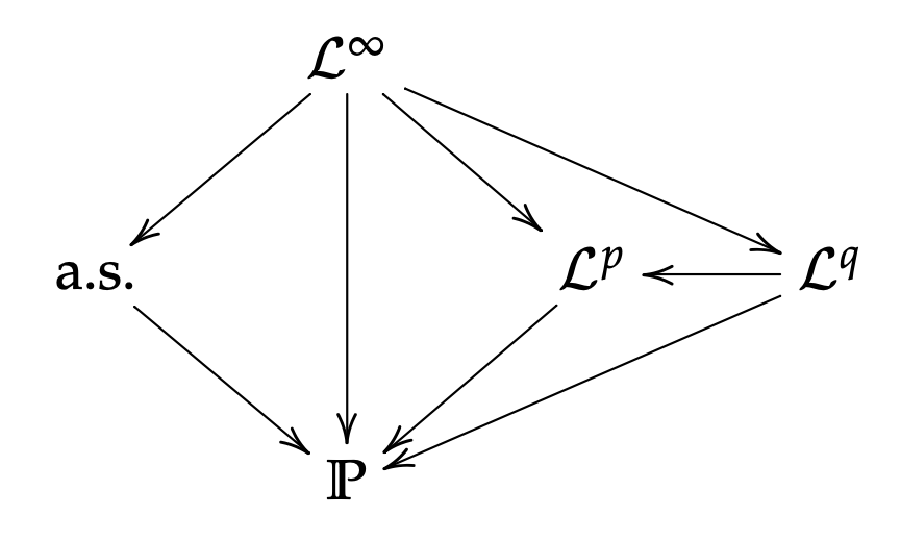
\includegraphics[scale=0.5]{1.eps}
    \end{center}
  \end{enumerate}

  \item Weak Convergence: If $S$ is a metric space with metric $d$ and $\mathcal{S} = \mathcal{B}(d)$, the $\sigma$-algebra generated by $d$, then for a sequence of probability measures $\bb{\mu_n}_n$ and $\mu$, $\mu_n \xrightarrow{w} \mu$ weakly convergent means
  \begin{equation*}
    \int f d\mu_n~ \longrightarrow ~ \int f d\mu,~\forall~f \in \mathcal{C}_b(S)
  \end{equation*}
  Let $(\Omega,\mathcal{F},\Pb)$ be a probability space. For a random variable $X \colon \Omega \sto \R$, the induced measure $\mu_X$ defined on $(\R,\mathcal{R})$ is
  \begin{equation*}
    \mu_X(A) = \Pb(X \in A),~\forall~A \in \mathcal{R}
  \end{equation*}
  So for a sequence of random variables $X_n$, the distribution convergence $X_n \xrightarrow{d} X$ means $\mu_{X_n} \xrightarrow{w} \mu_X$.

  \noindent Total-variation Convergence: a sequence of probability measures $\bb{\mu}_n$ over $(\R,\mathcal{R})$ converges $\mu$ in total-variation if
  \begin{equation*}
    \sup_{A \in \mathcal{R}}\abs{\mu_n(A) - \mu(A)} \sto 0,~\text{as } n\sto \infty
  \end{equation*}

  \item Characteristic Function over $\R$: For any probability measure $\mu$ on $(\R,\mathcal{R})$, the characteristic function is
  \begin{equation*}
    \phi_{\mu}(t) = \int e^{itx} \mu(dx)
  \end{equation*}
  For a random variable $X$, $\phi_{X} \def \phi_{\mu_X}$.
  \begin{enumerate}[label=(\arabic*)]
    \item If $\mu_n \xrightarrow{w} \mu$, then $\phi_{\mu_n}(t) \sto \phi_{\mu}(t)$ for all $t \in \R$.
    \item Continuity Theorem: Let $\bb{\mu_n}_n$ be probability measures and $\bb{\phi_n}_n$ be their characteristic functions. Suppose there is a $\phi$ such that $\phi$ is continuous at $t=0$ and $\phi_n \sto \phi$ for all $t$. Then $\phi$ is a characteristic function with probability measure $\mu$ and $\mu_n \xrightarrow{w} \mu$.
    \item Inversion problem: $\mu$ is a probability measure
    \begin{equation*}
      \mu((a,b)) + \frac{1}{2}\mu(\bb{a,b}) = \frac{1}{2\pi}\lim_{T \sto \infty}\int_{-T}^T\frac{e^{-iat} - e^{-ibt}}{it}\phi_{\mu}(t) dt
    \end{equation*}
    \item For two probability measure $\mu_1$ and $\mu_2$, $\phi_{\mu_1} = \phi_{\mu_2}$ implies $\mu_1 = \mu_2$.
    \item If $\int \abs{\phi_{\mu}(t)} dt < \infty$, then $\mu \ll \lambda$ and
    \begin{equation*}
      \frac{d\mu}{d\lambda} = f(x),~\text{where }f(x) = \frac{1}{2\pi}\int e^{-itx}\phi_{\mu}(x)dt
    \end{equation*}
    where $\lambda$ is the Lebesgue measure.
    \item Riemannian-Lebesgue theorem: If $\mu \ll \lambda$, then $\lim_{t\sto \pm\infty}\phi_{\mu}(t) = 0$
  \end{enumerate}

  \item Conditional Distribution: Let $(\mathcal{B},\norm{\cdot})$ be a Banach space and $(S,\mathcal{S})$ be measurable space. A map $\mu \colon S \sto B$ is called a vectored measure if $\mu(\varnothing)=0$ and 
  \begin{equation*}
    \mu\bc{\bigcup_nA_n} = \sum_n \mu(A_n),~\text{where }{A_n} \in \mathcal{S} \text{ disjoint}
  \end{equation*}
  So $A \mapsto \Pb(A \mid \mathcal{G}) \defeq \E[\mathds{1}_A \mid \mathcal{G}]$ is $L^1$-vectored measure.

  \noindent If $(E,\mathcal{E})$ and $(S,\mathcal{S})$ be two measurable spaces. A map $v \colon E \times \mathcal{S} \sto \R$ is called a (measurable) kernel if
  \begin{enumerate}[label=(\arabic*)]
    \item $x \mapsto v(x,B)$ is $\mathcal{E}$-measurable for each $B \in \mathcal{S}$;
    \item $B \mapsto v(x,B)$ is a measure on $S$ for each $x \in E$.
  \end{enumerate}

  \noindent For $e \colon \Omega \sto S$ measurable, $\mu_{e|\mathcal{G}} \colon \Omega \times \mathcal{S} \sto [0,1]$ is
  \begin{equation*}
    \mu_{e|\mathcal{G}}(\omega, B) \defeq \Pb(e \in B \mid \mathcal{G})(\omega)
  \end{equation*}
  is called the regular conditional distribution of $e$ given $\mathcal{G}$. If $(S,\mathcal{S}) = (\R,\mathcal{R})$ (or Borel space, \emph{i.e.} isomorphic in measure meaning to $(\R,\mathcal{R})$), then any $e$ introduces a regular conditional distribution. Let $\boldsymbol{X}$ be a $\R^n$-valued random vector and $g \colon \R^n \sto \R$ such that $g(\boldsymbol{X}) \in L^1$. Then
  \begin{equation*}
    \E\bj{g(\boldsymbol{X}) \mid \mathcal{G}} = \int_{\R^n} g(\boldsymbol{x})\mu_{\boldsymbol{X} | \mathcal{G}}(\cdot, d\boldsymbol{x})
  \end{equation*}
  More specifically,
  \begin{equation*}
    \mu_{\boldsymbol{X} | \mathcal{G}} \colon \Omega \times \mathcal{R}^n ~\longrightarrow~ [0,1]
  \end{equation*}
  \begin{enumerate}[label=(\arabic*)]
    \item Conditional cdf: $F_{\boldsymbol{X} | \mathcal{G}} \colon \Omega \times \R^n \sto [0,1]$ is defined by
    \begin{equation*}
      F(\omega, \boldsymbol{x}) = \mu_{\boldsymbol{X} | \mathcal{G}}(\omega, \bb{\boldsymbol{y} \colon\boldsymbol{y} \leqslant_n \boldsymbol{x}})
    \end{equation*}

    \item Conditional pdf: $f_{\boldsymbol{X} | \mathcal{G}} \colon \Omega \times \R^n \sto [0,\infty)$ satisfies
    \begin{enumerate}[label=(\roman*)]
      \item $f_{\boldsymbol{X} | \mathcal{G}}(\omega,\cdot)$ is Borel measurable for all $\omega \in \Omega$;
      \item $f_{\boldsymbol{X} | \mathcal{G}}(\cdot, \boldsymbol{x})$ is $\mathcal{G}$-measurable for each $\boldsymbol{x} \in \R^n$;
      \item $\int_A f_{\boldsymbol{X} | \mathcal{G}}(\omega, \boldsymbol{x})d\boldsymbol{x} = \mu_{\boldsymbol{X} | \mathcal{G}} (\omega, A)$ for $A \in \mathcal{R}^n$.
    \end{enumerate}

    \item Conditional characteristic function: $\phi_{\boldsymbol{X} | \mathcal{G}} \colon \Omega \times \R^n \sto \C$ is given by
    \begin{equation*}
      \phi_{\boldsymbol{X} | \mathcal{G}}(\omega, \boldsymbol{t}) = \int_{\R^n} e^{i\boldsymbol{t}\cdot\boldsymbol{x}}\mu_{\boldsymbol{X} | \mathcal{G}}(\omega, d\boldsymbol{x}),~\forall~\boldsymbol{t}\in\R^n,\omega \in \Omega
    \end{equation*}
    Moreover, $\phi_{\boldsymbol{X} | \mathcal{G}}(\omega, \boldsymbol{t}) = \phi(\boldsymbol{t})$ for some $\phi \colon \R^n \sto \C$ if and only if $\sigma(\boldsymbol{X})$ is independent with $\mathcal{G}$.
  \end{enumerate}

  \begin{thm}
    Let $\boldsymbol{X} = (\boldsymbol{X}^0,\boldsymbol{X}^u)$ be $\R^n$-vectored valued random variable, where $\boldsymbol{X}^0$ represents the first $d$ components and $\boldsymbol{X}^u$ represents the last components. Let $f_{\boldsymbol{X}} \colon \R^n \sto \R$ be the pdf of $\boldsymbol{X}$ and $\mathcal{G} =\sigma(\boldsymbol{X}^0)$. Then there is a conditional pdf
    \begin{equation*}
      f_{\boldsymbol{X}^u | \mathcal{G}}\colon \Omega \times \R^{n-d} \sto [0,\infty)
    \end{equation*}
    of $\boldsymbol{X}^u$ given $\mathcal{G}$,
    \begin{equation*}
      f_{\boldsymbol{X}^u \mid \mathcal{G}}\left(\omega, \boldsymbol{x}^u\right)= \begin{cases}\frac{f_{\boldsymbol{X}}\left(\boldsymbol{X}^o(\omega), \boldsymbol{x}^u\right)}{\int_{\mathbb{R}^{n-d}} f_{\boldsymbol{X}}\left(\boldsymbol{X}^o(\omega), \boldsymbol{y}\right) d \boldsymbol{y}}, & \int_{\mathbb{R}^{n-d}} f\left(\boldsymbol{X}^o, \boldsymbol{y}\right) d \boldsymbol{y}>0, \\ f_0\left(\boldsymbol{x}^u\right), & \text { otherwise, }\end{cases}
    \end{equation*}
    for $\boldsymbol{x} \in \R^{n-d}$ and $\omega \in \Omega$, where $f_0: \R^{n-d} \rightarrow \R$ is an arbitrary density function.
  \end{thm}

  \begin{thm}
    Suppose $\Omega,S$ are complete separable metric spaces with $\mathcal{F} = \mathcal{B}(\Omega)$. $Y \colon \Omega \sto Y$ is measurable and $\mu$ is the distribution of $Y$ on $S$. Then there is a measurable kernel
    \begin{equation*}
      P \colon S \times \mathcal{F} ~\longrightarrow~ [0,1]
    \end{equation*}
    such that
    \begin{equation*}
      P_x(A \backslash \bb{Y=x}) = 0,~a.e.~x \in S
    \end{equation*}
    and for any $X \in L^1(\Omega,S)$
    \begin{equation*}
      \E[X \mid Y](\omega) = \E_{Y(\omega)}[X] = \int_{\Omega}X(\omega)P_{x_0}(d\omega)
    \end{equation*}
    where $x_0=Y(\omega)$ and $\E_x$ is the expectation \emph{w.s.t.} $P_x$.
    \begin{rmk}
      It is a simplified version of above results.
    \end{rmk}
  \end{thm}
\end{itemize}

\section{Discrete Martingale}
\begin{itemize}
  \item Uniform Integrability: A family of random variables $\mathcal{X} \subset L^0$ is said UI if
  \begin{equation*}
    \lim_{K \sto \infty} \sup_{X \in \mathcal{X}}\E\bj{\abs{X}\mathds{1}_{\bb{\abs{X} > K}}} = 0
  \end{equation*}
  It is equivalent to $L^1$-bounded and uniformly absolutely continuous, \emph{i.e.}
  \begin{enumerate}[label=(\arabic*)]
    \item $\exists~C > 0$ such that $\E[\abs{X}] \leqslant C$ for all $X \in \mathcal{X}$
    \item $\forall~\varepsilon > 0,~\exists~\delta > 0$ such that for any $A \in \mathcal{F}$,
    \begin{equation*}
      \Pb(A) < \delta ~\Rightarrow~ \sup_{X \in \mathcal{X}}\E\bj{\abs{X}\mathds{1}_A} \leqslant \varepsilon
    \end{equation*}
  \end{enumerate}
  Or if there is a function $\varphi \colon [0,\infty) \sto [0,\infty)$ with $\lim_{x\sto \infty} \varphi(x) / x = \infty$ such that
  \begin{equation*}
    \sup_{X \in \mathcal{X}}\E\bj{\varphi(\abs{X})} < \infty
  \end{equation*}
  then $\mathcal{X}$ is UI. So $\sup_{X \in \mathcal{X}}\norm{X}_{L^p} < \infty$ ($p>1$) implies UI.

  \noindent If $\bb{\mathcal{X}_n}_{n\in \N_0} \subset L^p$ ($p\geqslant 1$) and $X \in L^0$ with $X_n \xrightarrow{\Pb} X$, then 
  \begin{equation*}
    \bb{\mathcal{X}_n}_{n\in \N_0}~\text{UI}~\Leftrightarrow~X_n \xrightarrow{L^p} X ~\Leftrightarrow~\norm{X_n}_{L^p} \sto \norm{X} < \infty
  \end{equation*}

  \item Discrete Martingale: Fix a discrete filtered probability $(\Omega, \mathcal{F}, (\mathcal{F}_n)_{n\in \N_0}, \Pb)$. Let $X=(X_n)_{n\in \N_0}$ be a discrete stochastic process.
  \begin{enumerate}[label=(\arabic*)]
    \item $X$ is adapted if $X_n$ is $\mathcal{F}_n$-measurable for $n\in \N_0$.
    \item $X$ is predicted if $X_n$ is $\mathcal{F}_{n-1}$-measurable for $n\in \N$.
  \end{enumerate}

  \noindent Let $X$ and $H$ be two discrete stochastic processes. $\bc{(H\cdot X)_n}_{n\in \N_0}$ is defined by
  \begin{equation*}
    (H\cdot X)_0 = 0,~(H\cdot X)_n \defeq \sum_{k=1}^nH_k(X_k-X_{k-1}),~\forall~n\in \N
  \end{equation*}
  called the martingale transform of $X$ by $H$. Moreover, if $H$ is predictable and $H_n(X_n-X_{n-1}) \in L^1$, then $X$ (sub)-martingale implies $H\cdot X$ (sub)-martingale. Note that it is the discrete version of stochastic integral.

  \noindent There are some properties of stopping times.
  \begin{enumerate}[label=(\arabic*)]
    \item A random time $T$ is stopping time if and only if the process $X_n = \mathds{1}_{\bb{n \geqslant T}}$ is adapted.
    \item If $S$ and $T$ are stopping times, then $S+T$ and $\max{S,T}$ and $\min{S,T}$ are stopping times.
    \item If $\bb{T_n}_{n\in \N_0}$ is a sequence of stopping times with $T_1 \leqslant T_2 \leqslant \cdots$ \emph{a.s.}, then $T = \sup_n T_n$ is also a stopping time. (Similarly for decreasing and $\inf$).
  \end{enumerate}

  \begin{exam}[Stopping Times]
    \item For a fixed $m \in \N_0 \cup \bb{\infty}$, let $T = m$ be the constant random time so it is clear a stopping time.
    \item Let $(X_n)_{n \in \N_0}$ be a $(\mathcal{F}_n)_{n \in \N_0}$-adopted process, then for a fixed Borel set $B$ 
    \begin{equation*}
      T_B \defeq \min\bb{n \in \N_0 \colon X_n \in B}
    \end{equation*}
    is a stopping time because
    \begin{equation*}
      \bb{T_B \leqslant n} = \bb{X_0 \in B} \cup \bb{X_1 \in B} \cup \cdots \cup \bb{X_n \in B}
    \end{equation*}
  \end{exam}

  \noindent Let $X=(X_n)_{n\in \N_0}$ be a stochastic process and $T$ be a stopping time. The process $X^T=(X_n^T)_{n\in \N_0}$ is called $X$ stopped at $T$, defined as
  \begin{equation*}
    X^T_n(\omega) \defeq X_{T(\omega)\wedge n} = X_n(\omega)\mathds{1}_{\bb{n \leqslant T(\omega)}} +  X_{T(\omega)}\mathds{1}_{\bb{n > T(\omega)}}
  \end{equation*}
  Note that $X$ (sub)martingale implies $X^T$ (sub)martingale.

  \begin{thm}[Martingale Convergence]
    Let $X=(X_n)_{n\in \N_0}$ be a martingale with
    \begin{equation*}
      \sup_{n}\E\bj{\abs{X_n}} < \infty
    \end{equation*}
    Then there is a random variable $X^* \in L^1$ such that $X_n \sto X$ \emph{a.e.}.
  \end{thm}

  \begin{prop}[Doob-Meyer Decomposition]
    Let $X=(X_n)_{n\in \N_0}$ be a submartingale. There exists a martingale $M$ and a predictable $A$ with $A_0 = 0$ such that $A_n \in L^1$ and $A_n \leqslant A_{n+1}$ and
    \begin{equation*}
      X_n = M_n + A_n
    \end{equation*}
  \end{prop}
  Here
  \begin{equation*}
    A_n \defeq \sum_{k=1}^n\E\bj{X_k - X_{k-1} \mid \mathcal{F}_{k-1}},~n\in \N
  \end{equation*}
  and $M_n = X_n - A_n$. Predictability of $A_n$ is clear and $A_{n+1} \geqslant A_n$ is by the submartingale property of $X_n$. And $\E[M_n - M_{n-1} \mid \mathcal{F}_{n-1}] = 0$ by simply calculating.

  \noindent Then for a submartingale with $\sup_{n}\E\bj{X_n^+} < \infty$, then there is a $X^* \in L^1$ such that $X_n \sto X^*$ \emph{a.e.}. Moreover, if (sub)martingale $\bb{{X}_n}_{n\in \N_0}$ is UI, then $X_n \xrightarrow{L^1} X^*$ because $X_n \in L^1$ and $X_n \sto X^*$ \emph{a.e} implies $X_n \xrightarrow{\Pb} X^*$. 

  \noindent A martingale $X$ is called a L\'evy martingale if there is a random variable $\tilde{X} \in L^1$ such that $X_n = \E[\tilde{X} \mid \mathcal{F}_n]$ for every $n \in \N_0$. A martingale $X$ is L\'evy if and only if it is UI. And thus it has a $L^1$-limit, that is $\E[\tilde{X} \mid \mathcal{F}_{\infty}]$, where $ \mathcal{F}_{\infty} = \sigma(\cup_n\mathcal{F}_n)$.

  \item Backward Martingale: Let $-\N_0 = \bb{\cdots,-2,-1,0}$. Filtration $\bc{\mathcal{F}_n}_{n\in -\N_0}$ is $\sigma$-algebras with $\mathcal{F}_{n-1} \subset \mathcal{F}_n$. A stochastic process $\bc{X_n}_{n\in -\N_0}$ is called backward submartingale with respect to $\bc{\mathcal{F}_n}_{n\in -\N_0}$ if it is adapted and in $L^1$ and
  \begin{equation*}
    \E[X_n \mid \mathcal{F}_{n-1}] \geqslant X_{n-1},~\forall~n\in -\N_0
  \end{equation*}
  $\bc{X_n}_{n\in -\N_0}$ is called backward supermartingale if $\bc{-X_n}_{n\in -\N_0}$ is a backward submartingale. When taking the equality, it is a backward martingale.

  \begin{thm}
    Suppose $\bc{X_n}_{n\in -\N_0}$ is a backward submartingale such that
    \begin{equation*}
      \lim_{n \sto -\infty}\E[X_n] > -\infty
    \end{equation*}
    Then $\bb{X_n}_{n\in -\N_0}$ is UI and there is a $X_{-\infty} \in L^1(\cap_n\mathcal{F}_n)$ such that
    \begin{equation*}
      X_n \sto X_{-\infty}
    \end{equation*}
    \emph{a.e.} and in $L^1$. Moreover,
    \begin{equation*}
      X_{-\infty} \leqslant \E\bj{X_m \mid \cap_n\mathcal{F}_n},~\forall~m\in \N_0
    \end{equation*}
  \end{thm}

  \noindent If $\bc{X_n}_{n\in -\N_0}$ is a backward martingale, then
  \begin{equation*}
    X_n \sto X_{-\infty} = \E[X_0 \mid \cap_n\mathcal{F}_n]
  \end{equation*}
  \emph{a.e} and in $L^1$.

  \item Maximal Process:  A random variable $Y$ is called weak $L^1$ ($wL^1$) if there is $C\geqslant 0$ such that 
  \begin{equation*}
    \lambda\Pb(\abs{Y} > \lambda) \leqslant C,~\forall~\lambda > 0
  \end{equation*}
  and the smallest $C$ is called $\norm{Y}_{wL^1}$. Note that it is not a norm. Besides, by the Markov's inequality, $L^1 \subset wL^1$.

  \noindent For a stochastic process $\bc{X_n}_{n\in \N_0}$, the maximal process is $\bc{X_n^*}_{n\in \N_0}$ defined as
  \begin{equation*}
    X_n^* = \sup_{0\leqslant m \leqslant n}\abs{X_m}
  \end{equation*}
  and $X_{\infty}^* = \sup_{n}\abs{X_n}$. By the Doob's Inequality, if $\bc{X_n}_{n\in \N_0}$ is a martingale or non-negative submartingale, then
  \begin{equation*}
    \Pb(X_n^* \geqslant \lambda) \leqslant \frac{\E[\abs{X_n}\mathds{1}_{\bb{X_n^* \geqslant \lambda}}]}{\lambda} \leqslant \frac{\E[\abs{X_n}]}{\lambda}
  \end{equation*} 
  for any $n \in \N_0$ and $\lambda > 0$. And it implies
  \begin{equation*}
    \norm{X_{\infty}^*}_{wL^1} \leqslant \sup_{n \in \N_0}\norm{X_n}_{L^1}
  \end{equation*}
  \begin{thm}[Maximal Inequality]
    Let $\bc{X_n}_{n\in \N_0}$ be a martingale or non-negative submartingale, and $p \in (1,\infty)$. Then, for $n \in \N_0$,
    \begin{equation*}
      \norm{X_n^*}_{L^p} \leqslant \frac{p}{p-1}\norm{X_n}_{L^p}
    \end{equation*}
  \end{thm}

  \noindent A stochastic process $\bc{X_n}_{n\in \N_0}$ is said bounded in $L^p$ for $p\in [1,\infty]$ if
  \begin{equation*}
    \sup_n \norm{X_n}_{L^p} < \infty
  \end{equation*}
  If $\bc{X_n}_{n\in \N_0}$ is a martingale or non-negative submartingale, and $L^p$-bounded for $(1,\infty)$, then
  \begin{enumerate}[label=(\arabic*)]
    \item the family $\bb{\abs{X_n}}_{n\in \N_0}$ is UIs,
    \item there exists a $X_{\infty} \in L^p$ such that $X_n \sto X_{\infty}$ in $L^p$.
  \end{enumerate}

  \item Stopping Time Theorems: Let $T$ be a stopping time and $\bc{X_n}_{n\in \N_0}$ be a stochastic process. When $\Pb(T = \infty) = 0$, 
  \begin{equation*}
    X_T(\omega) \defeq X_{T(\omega)}(\omega)
  \end{equation*}
  But if $\Pb(T = \infty) \neq 0$
  \begin{equation*}
    X_T \defeq \lim_{n\sto \infty}X_{T \wedge n}
  \end{equation*}
  when the limit exists \emph{a.e.}.

  \begin{prop}[UI conditions]
    For a martingale $\bc{X_n}_{n\in \N_0}$, let $T$ be a stopping time such that $\bc{X^T_n}_{n\in \N_0}$ is UI, then 
    \begin{equation*}
      X_T = \lim_{n\sto \infty}X_{T \wedge n} \in L^1~a.e.~,~\E[X_T] = \E[X_0] \tag{$1$}
    \end{equation*}
    Conversely, if $\bc{X_n}_{n\in \N_0}$ is a nonnegative martingale and $T$ is a stopping time such that $(1)$ holds, then $\bc{X^T_n}_{n\in \N_0}$ is UI.
  \end{prop}

  \noindent In fact, for a martingale $\bc{X_n}_{n\in \N_0}$ and a stopping time $T$, each of the following situations can make $\bc{X^T_n}_{n\in \N_0}$ be UI.
  \begin{enumerate}[label=\Roman*.]
    \item $T$ is bounded.
    \item $X$ is UI.
    \item $\E[T] < \infty$ and there is a $C> 0$ such that $\E[\abs{X_{n+1}-X_n} \mid \mathcal{F}_n] < C$ for all $n$.
  \end{enumerate}

  \begin{prop}
    Let $\bc{X_n}_{n\in \N_0}$ be a nonnegative supermartingale and $T$ be a stopping time. Then $X_T = \lim_{n}X_{T \wedge n}$ is well-defined, $X_T \in L^1$ and $\E[X_T] \leqslant \E[X_0]$. If $\bc{X_n}_{n\in \N_0}$ is a submartingale and $\bb{X_{T \wedge n}^+}_n$ is UI, then $X_T \in L^1$ is well-defined and $\E[X_T] \geqslant \E[X_0]$.
  \end{prop}

  For a stopping time $T$, let
  \begin{equation*}
    \mathcal{F}_T = \bb{A \in \mathcal{F}_{\infty} \colon A \cap \bb{T \leqslant n} \in \mathcal{F}_n,~\forall~n\in \N_0}
  \end{equation*}
  where $\mathcal{F}_{\infty} = \sigma(\cup_n\mathcal{F}_n)$. Then $\mathcal{F}_T$ is the $\sigma$-algebra generated by
  \begin{equation*}
    \mathcal{S} = \bb{X_T \colon X \in \mathcal{X}}
  \end{equation*} 
  where $\mathcal{X}$ is the set of all $\mathcal{F}_n$-adapted process for which $X_T$ is well-defined.

  \begin{prop}
    Let $\bc{X_n}_{n\in \N_0}$ be a UI martingale and $S,T$ be two stopping times with $T \leqslant S$ \emph{a.e.}. Then $X_T, X_S \in L^1$ and 
    \begin{equation*}
      \E[X_S \mid \mathcal{F}_T] = X_T,~a.e
    \end{equation*}
    In particular,
    \begin{equation*}
      \E[X_S] = \E[X_T]
    \end{equation*}
  \end{prop}

  \item Square-integrability: A martingale $\bc{X_n}_{n\in \N_0}$ is called a $L^2$-martingale if $X_n \in L^2$ for all $n \in \N_0$. For any $m_2 > n_2 \geqslant m_1 > n_1$,
  \begin{equation*}
    \E[(X_{m_2}-X_{n_2})(X_{m_1}-X_{n_1}) \mid \mathcal{F}_{n_1}] = 0
  \end{equation*}
  In particular, $X_{m_2}-X_{n_2}$ is orthogonal to $X_{m_1}-X_{n_1}$ in $L^2$. Moreover,
  \begin{equation*}
    \E[(X_{m_1}-X_{n_1})^2 \mid \mathcal{F}_{n_1}] = \E[X_{m_1}^2-X_{n_1}^2 \mid \mathcal{F}_{n_1}] 
  \end{equation*}

  \noindent $L^2$-martingale $\bc{X_n}_{n\in \N_0}$ implies that $\bc{X_n^2}_{n\in \N_0}$ is submartingale. So by the Doob-Meyer decomposition, there are a martingale $M_n$ and a predictable process $A_n$ that is denoted by $\inn{X}_n$. By the construction of $A_n$ and the property of $L^2$-martingale,
  \begin{equation*}
    \inn{X}_n - \inn{X}_{n-1} = \E\bj{(X_n-X_{n-1})^2 \mid \mathcal{F}_{n-1}}
  \end{equation*}
  called the quadratic variation. And define $\inn{X}_{\infty} = \lim_{n\sto \infty}\inn{X}_n \in [0,\infty]$, and it is well-defined because $\inn{X}_n$ is increasing. Then $\bc{X_n}_{n\in \N_0}$ is $L^2$-bounded if and only if $\E[\inn{X}_{\infty}] < \infty$. In such case,
  \begin{equation*}
    \E[(X_{\infty}^*)^2] \leqslant \E[X_0^2] + 4\E[\inn{X}_{\infty}]
  \end{equation*}

  \begin{prop}
    Let $\bc{X_n}_{n\in \N_0}$ be $L^2$ martingale. Then on $\bb{\inn{X}_{\infty} < \infty}$, $\lim_n X_n$ exists.
  \end{prop}
  \begin{proof}
    For $N \in \N$, define a random time
    \begin{equation*}
      T_N = \min\bb{n \in \N_0\colon \inn{X}_{n+1} \geqslant N}
    \end{equation*}
    Because $\inn{X}$ is predictable, $T_N$ is a stopping time. And since $X^2-\inn{X}$ is a martingale, by the bounded optional stopping theorem
    \begin{equation*}
      \E[X^2_{T_N \wedge n}] = \E[X_0^2] + \E[\inn{X}_{T_N \wedge n}]
    \end{equation*}
    And because $\inn{X}_n$ increasing, $\inn{X}_{T_N \wedge n} \leqslant N$ for any $N$ and $n$. Therefore,
    \begin{equation*}
      \E[X^2_{T_N \wedge n}] \leqslant \E[X_0^2] + N
    \end{equation*}
    So the martingale $(X^{T_N}_n)_{n\in \N_0}$ is $L^2$-bounded. In particular, $\lim_nX^{T_N}_n$ exists.

    For almost all $\omega \in \bb{\inn{X}_{\infty} < \infty}$, there is a sufficiently large $N$ such that $T_N(\omega) = \infty$. So choose such $N$, then $X^{T_N}_n =X_n$.
  \end{proof}
\end{itemize}

\section{Brownian Motion}
\begin{itemize}
  \item Gaussian Measure: A measure $\gamma$ on $\R^n$ is called Gaussian if its characteristic function is
  \begin{equation*}
    \varphi_{\gamma}(\bd{t}) = \exp(i\bd{t}^T\bd{\mu}-\frac{1}{2}\bd{t}^T\bd{\Sigma}\bd{t})
  \end{equation*}
  where $\bd{t} \in \R^n$ and $\bd{\Sigma} \in \R^{n\times n}$ is a positive semi-definite matrix. A $\R^n$-valued random vector $\bd{X}$ is called Gaussian if $\mu_{\bd{X}} = \gamma$.

  \begin{thm}[Structure Theorem of Gaussian]
    TFAE for a random vector $\bd{X} \colon \Omega \sto \R^n$.
    \begin{enumerate}[label=(\arabic*)]
      \item $\bd{X}$ is Gaussian.
      \item For each $\bd{a} \in \R^n$, the linear combination $\bd{a}^T\bd{X}$ is Gaussian.
      \item Either $\bd{X}$ is constant or there exist
      \begin{enumerate}[label=(\roman*)]
        \item an integer $d \in \N$,
        \item a vector $\bd{\mu} \in \R^n$,
        \item a rank $d$ matrix $\bd{A} \in \R^{n \times d}$,
        \item a $\R^d$-valued $\bd{Y}$ defined on the same probability space as $\bd{X}$ and with the standard $d$-dimensional Gaussian
      \end{enumerate}
      such that
      \begin{equation*}
        \bd{X} = \bd{\mu} + \bd{A}\bd{Y}
      \end{equation*}
    \end{enumerate}
  \end{thm}
  \begin{rmk}
    Then support of $\bd{X}$ is the affine space
    \begin{equation*}
      \bd{\mu} + \Img \bd{\Sigma} = \bb{\bd{\mu} + \bd{\Sigma}\bd{x} \colon \bd{x} \in \R^n}
    \end{equation*}
    In fact, $d = \rank \bd{\Sigma}$, called the rank of the Gaussian. If $d = n$, it is called nondegenerate, otherwise, it is degenerate. $\bd{X}$ is nondegenerate if and only if it admits a pdf
    \begin{equation*}
      f_{\bd{X}}(\bd{x})=\frac{1}{\sqrt{(2 \pi)^n \operatorname{det} \boldsymbol{\Sigma}}} \exp \left(-\frac{1}{2}(\bd{x}-\bd{\mu})^T \boldsymbol{\Sigma}^{-1}(\bd{x}-\bd{\mu})\right)
    \end{equation*}
  \end{rmk}

  \noindent An $n$-dimensional random vector $\bd{X}$ defined on $(\Omega, \mathcal{F}, \Pb)$ is called conditionally normally distributed with respect to a $\sigma$-subalgebra $\mathcal{G} \subset \mathcal{F}$ if there exist
  \begin{enumerate}[label=(\Roman*)]
    \item a random vector $\bd{\mu}_{\bd{X}|\mathcal{G}}$,
    \item a random $n \times n$ matrix $\bd{\Sigma}_{\bd{X}|\mathcal{G}}$, that is positive semi-definite,
  \end{enumerate}
  such that $\bd{\mu}_{\bd{X}|\mathcal{G}}$ and $\bd{\Sigma}_{\bd{X}|\mathcal{G}}$ are $\mathcal{G}$-measurable and 
  \begin{equation*}
    \E[e^{i\bd{t}^T\bd{x}} \mid \mathcal{G}] = \exp\bc{i\bd{t}^T\bd{\mu}_{\bd{X}|\mathcal{G}} - \frac{1}{2}\bd{t}^T\bd{\Sigma}_{\bd{X}|\mathcal{G}}\bd{t}}
  \end{equation*}
  \begin{rmk}
    We can let
    \begin{equation*}
      \bd{\mu}_{\bd{X}|\mathcal{G}} = \E[\bd{X} \mid \mathcal{G}],~\bd{\Sigma}_{\bd{X}|\mathcal{G}} =  \E \bj{(\bd{X}-\bd{\mu}_{\bd{X}|\mathcal{G}})^T(\bd{X}-\bd{\mu}_{\bd{X}|\mathcal{G}}) \mid \mathcal{G}}
    \end{equation*}
    Note that $\bd{X}$ is independent with $\mathcal{G}$ if and only if $\bd{\mu}_{\bd{X}|\mathcal{G}}$ and $\bd{\Sigma}_{\bd{X}|\mathcal{G}}$ are constant.
  \end{rmk}

  \item Brownian Motion: Let $(B_t)_{t \geqslant 0}$ be a Brownian motion, \emph{i.e.}
  \begin{enumerate}[label=(\arabic*)]
    \item $B_0 = 0$ \emph{a.e.} and $B_t -B_s \sim \mathcal{N}(0, t-s)$ for all $0\leqslant s < t$;
    \item $(B_t)_{t \geqslant 0}$ is independent increments.
    \item $\exists~\Omega^*$ with $\Pb(\Omega^*)=1$ such that $t \mapsto B_t(\omega)$ is continuous for all $\omega \in \Omega^*$.
  \end{enumerate}

  The existence of Brownian motion is based on the following theories.
  \begin{enumerate}[label=(\arabic*)]
    \item The Kolmogorov Extension Theorem: Let $\mathcal{T}$ be a nonempty index set, and
    \begin{equation*}
      \bb{\mu_{t_1,t_2,\cdots,t_n} \colon n \in \N,~t_1,t_2,\cdots,t_n\in \mathcal{T}}
    \end{equation*}
    be a family of probability measures on $\R^n$ with the property
    \begin{enumerate}[label=(\roman*)]
      \item $\forall~n\in \N$, $(t_1,t_2,\cdots,t_n) \in \mathcal{T}^n$ and a permutation $\sigma \in S_n$ and $\bb{A_i}_{i=1}^n \in \mathcal{R}$
      \begin{equation*}
        \mu_{(t_1,\cdots,t_n)}(A_1\times\cdots\times A_n) = \mu_{(t_{\sigma(1)},\cdots,t_{\sigma(n)})}(A_{\sigma(1)}\times\cdots\times A_{\sigma(n)})
      \end{equation*}

      \item $\forall~n\in\N$ and $A \in \mathcal{R}^n$ and $(t_1,t_2,\cdots,t_{n+1}) \in \mathcal{T}^{n+1}$,
      \begin{equation*}
        \mu_{(t_1,\cdots,t_{n+1})}(A\times\R) = \mu_{(t_1,\cdots,t_n)}(A)
      \end{equation*}
    \end{enumerate}
    Then there is a probability measure $\Pb$ defined on
    \begin{equation*}
      \bc{\prod_{t\in \mathcal{T}} \R, \prod_{t\in \mathcal{T}}\mathcal{R}}
    \end{equation*}
    such that the finite-dimensional distribution of the coordinate process $\bb{x_t}_{t \in \mathcal{T}}$ is given by $\mu$.
    \begin{defn}
      For $n \in$ $\mathbb{N}$, the family of probability measures $\mu_{t_1, \ldots, t_n}$ on $\mathcal{B}\left(\mathbb{R}^n\right)$ indexed by all $n$-tuples $\left(t_1, \ldots, t_n\right) \in[0, \infty)^n$ is said to be the (family of) $n$-dimensional distributions of the stochastic process $\left\{\bd{X}_t\right\}_{t \in[0, \infty)}$ if
      \begin{equation*}
        \mu_{t_1, \ldots, t_n}(x_1,\cdots,x_n) = \Pb\bc{\bb{\omega \in \Omega \colon \bd{X}_{t_i}(\omega) \leq x_i,~\forall~i}}
      \end{equation*}
      for all $t_1, \ldots, t_n \in[0, \infty)$. The collection of all $n$-dimensional distribution, with $n$ ranging through $\mathbb{N}$ is called the (family of) finite-dimensional distributions of the process $\left\{\bd{X}_t\right\}_{t \in[0, \infty)}$.
    \end{defn}
    \begin{rmk}
      Note that for $A = A_1 \times \cdots \times A_n$
      \begin{equation*}
        \Pb\bc{(\bd{X}_{t_1},\bd{X}_{t_2},\cdots , \bd{X}_{t_n})^{-1}(A)} = \Pb\bc{\bd{X}_{t_1}\in A_1,\bd{X}_{t_2}\in A_2,\cdots,\bd{X}_{t_n}\in A_n}
      \end{equation*}
      because
      \begin{equation*}
        (\bd{X}_{t_1},\bd{X}_{t_2},\cdots , \bd{X}_{t_n})^{-1}(A) = \bigcap_{i=}^n\bd{X}^{-1}_{t_i}(A_i)
      \end{equation*}
      So
      \begin{equation*}
        \mu_{t_1, \ldots, t_n}(x_1,\cdots,x_n) = \Pb\bc{\bd{X}_{t_1}\leq x_1,\bd{X}_{t_2}\leq x_2,\cdots,\bd{X}_{t_n}\leq x_n}
      \end{equation*}
      which means it is the joint distribution of $\bc{\bd{X}_{t_1},\cdots,\bd{X}_{t_n}}$.
    \end{rmk}

    \noindent Therefore, there is a probability space $(\Omega,\mathcal{F},\Pb)$ supporting a process $(X_t)_{t \geqslant 0}$ which satisfies $(1)(2)$ for the definition of Brownian motion by letting $\mu_{(t_1,\cdots,t_n)}$ be a centered Gaussian measure on $\R^n$ with covariance $\Sigma_{ij} = \min \bb{t_i,t_j}$.

    \item For $(3)$, a real function $f \colon [0,\infty) \sto \R$ is said local H\"older continuous with $\gamma \in (0,1]$ if $\exists~\delta,K>0$ such that
    \begin{equation*}
      \abs{f(t)-f(s)} \leqslant K\abs{t-s}^{\gamma},~\forall~t,s\text{ with }\abs{t-s}<\delta
    \end{equation*}
    
    \noindent Kolmogorov-C\v{e}ntsov Theorem: If a stochastic process $(X_t)_{t \in [0,1]}$ satisfies
    \begin{equation*}
      \E[\abs{X_t -X_s}^{\alpha}] \leqslant C\abs{t-s}^{1+\beta}
    \end{equation*}
    for some $\alpha,\beta,C> 0$. Then there is modification $(\tilde{X}_t)_{t \in [0,1]}$ on $\Omega^*$ such that for $\omega \in \Omega^*$, $t \mapsto \tilde{X}_t(\omega)$ is $\gamma$-local H\"older continuous for $0 < \gamma < \frac{\beta}{\alpha}$.

    \noindent Because $X_t - X_s \sim \mathcal{N}(0, t-s)$ and $X_1 \sim \mathcal{N}(0,1)$,
    \begin{equation*}
      \E[\abs{X_t-X_s}^{2n}] = C_n\abs{t-s}^n
    \end{equation*}
    where $C_n = \E[\abs{X_1}^{2n}] = \frac{(2n)!}{2^nn!} < \infty$, there is a modification satisfying the continuous path condition. So $(B_t)_{t\in [0,1]}$ is a Brownian motion. This Brownian motion can be extended to $[0,\infty)$.
  \end{enumerate}

  \item Canonical Space: Equipping $\mathcal{C}([0,\infty))$ with the uniform continuous topology that is $\alpha_n \sto \alpha$ if $\alpha_n|_{[0,k]} \sto \alpha|_{[0,k]}$ uniformly for all $k \in \N$. Moreover, this topology is metrizable wit a metric $d$. $(\mathcal{C}([0,\infty)),d)$ is separable and complete. And let $\mathcal{B}(\mathcal{C}([0,\infty)))$ be the Borel algebra generated by this topology. 

  \noindent For any $t \in [0,\infty)$, let $\pi_t \colon \mathcal{C}([0,\infty)) \sto \R$ by $\pi_t(\alpha)=\alpha(t)$. Fix $n\in \N$ and $A \in \mathcal{R}^n$ and $t_1,\cdots,t_n \geqslant 0$,
  \begin{equation*}
    \bb{\alpha \in \mathcal{C}([0,\infty)) \colon (\alpha(t_1),\alpha(t_2),\cdots,\alpha(t_n)) \in A}
  \end{equation*}
  is called a finite-dimensional cylinder. Let $\mathcal{C}$ be the set of all finite-dimensional cylinders. In fact, $\mathcal{B}(\mathcal{C}([0,\infty))) = \sigma(\mathcal{C})$. Moreover, it is also the smallest $\sigma$-algebra such that all $\pi_t$ are measurable.

  \begin{prop}
    Let stochastic process $X=(X_t)_{t\geqslant 0}$ be path-continuous. Then there exists a probability measure $\Pb_X$ define on $\mathcal{C}([0,\infty)$ such that the coordinate process $\bc{x_t}_{t\geqslant 0}$ has the same finite-dimensional distributions as $(X_t)_{t \geqslant 0}.$
  \end{prop}
  \begin{rmk}
    Since $X=(X_t)_{t\geqslant 0}$ is path-continuous, it can be viewed as a measurable map
    \begin{equation*}
      X \colon (\Omega,\mathcal{F}) ~\longrightarrow~(\mathcal{C}([0,\infty)),\sigma(\mathcal{C}))
    \end{equation*}
    Therefore, $\Pb_X$ defined on $\mathcal{C}([0,\infty))$ is the push-forward probability measure of $\Pb$ with respect to $X$.
  \end{rmk}
  Such $\Pb_X$ is called the law or the distribution of $X$. In particular, if $X$ is a Brownian motion, then $\Pb_X$ is called a Wiener measure (because Brownian motion is also called Wiener process).

  \item More for path space $\mathcal{C}([0,T],\R^d)$: On $\mathcal{C}([0,T],\R^d)$, for any $t \in [0,T]$, let
  \begin{equation*}
    \begin{array}{cccl}
    \vspace{0.5em}
      \pi_t \colon &\mathcal{C}([0,T],\R^d)& \longrightarrow & \R^d\\
      ~&(\alpha(t))_{t \in [0,T]} &\mapsto & \pi_t\bc{(\alpha(t))_{t \in [0,T]}} \defeq \alpha(t)
    \end{array}
  \end{equation*}
  and as above mention define the set of Borel sets $\mathcal{B} = \mathcal{B}(\mathcal{C}([0,T],\R^d))$ be the smallest set such that each $\pi_t$ is measurable and also it is generated by the finite cylinders. Next, let's see its connections to random process

  \begin{enumerate}[label=(\arabic*)]
    \item For a process $\bd{X} = (\bd{X}_t)_{t \in [0,T]}$ over $(\Omega, \Pb, \mathcal{F})$, $\bd{X}$ can be viewed as
    \begin{equation*}
      \begin{array}{cccc}
      \vspace{0.5em}
        \bd{X} \colon &(\Omega,\mathcal{F})& \longrightarrow &\bc{\mathcal{C}([0,T],\R^d),\mathcal{B}} \\
        ~&\omega &\mapsto & (\bd{X}_t(\omega))_{t \in [0,T]}
      \end{array}
    \end{equation*}
    and by the definition of $\mathcal{B}$ (finite cylinders), $\bd{X}$ is measurable because for any $\prod_{i=1}^nA_i$ ($A_i \in \mathcal{R}^d$),
    \begin{equation*}
      \begin{array}{ll}
        \vspace{0.8em}
        ~&\quad \bd{X}^{-1}\bc{\bb{\alpha \in \mathcal{C}([0,\infty), \R^d) \colon (\alpha(t_1),\alpha(t_2),\cdots,\alpha(t_n)) \in \prod_{i=1}^nA_i}}\\\vspace{0.8em}
        ~&= \bd{X}^{-1}\bc{\bb{\alpha \in \mathcal{C}([0,\infty), \R^d) \colon \alpha(t_i) \in A_i,~i=1,2,\cdots,n}} \\\vspace{0.8em}
        ~&= \bb{\omega \in \Omega \colon \bd{X}_{t_i}(\omega) \in A_i,~i=1,2,\cdots,n} \\
        ~&== \bigcap_{i=}^n\bd{X}^{-1}_{t_i}(A_i) \in \mathcal{F}
      \end{array}
    \end{equation*}
    For $\bd{X}$, define $\Pb_X$ over $\mathcal{C}([0,\infty), \R^d)$ by push-forward $\Pb_X = \bd{X}_{\#}\Pb $. Therefore, for
    \begin{equation*}
      C = \bb{\alpha \in \mathcal{C}([0,\infty), \R^d) \colon (\alpha(t_1),\alpha(t_2),\cdots,\alpha(t_n)) \in \prod_{i=1}^nA_i } \in \mathcal{B}
    \end{equation*}
    we have
    \begin{equation*}
      \Pb_X(C) = \Pb(\bd{X} \in  C) = \Pb(\bd{X}^{-1}(C))
    \end{equation*}

    \item Next, let research $\Pb_X$ from another view.  Let $\pi = (\pi_t)_{t \in [0,T]}$ be the process defined as above on $\mathcal{C}([0,T],\R^d)$, called the coordinate process. Then for any measure $\mu$ on $\mathcal{C}([0,T],\R^d)$, let's consider the finite-dimensional distribution of $\pi$ given by $\mu$. For $0\leq t_1<t_2<\cdots < t_n \leq T$, 
    \begin{equation*}
      \begin{array}{cccl}
      \vspace{0.5em}
        (\pi_{t_1},\pi_{t_2},\cdots , \pi_{t_n}) \colon &\mathcal{C}([0,T],\R^d)& \longrightarrow & \prod_{i=1}^n\bc{\R^d}\\
        ~&(\alpha(t))_{t \in [0,T]} &\mapsto & (\alpha(t_1),\alpha(t_2),\cdots , \alpha(t_n))
      \end{array}
    \end{equation*}
    Then define $\mu_{t_1,t_2,\cdots , t_n} = (\pi_{t_1},\pi_{t_2},\cdots , \pi_{t_n})_{\#}\mu$, that is, for $A=\prod_{i=1}^nA_i \in \bc{\mathcal{R}^d}^n$,
    \begin{equation*}
      \mu_{t_1,t_2,\cdots , t_n}(A) \defeq \mu\bc{(\pi_{t_1},\pi_{t_2},\cdots , \pi_{t_n})^{-1}(A)} = \mu\bc{\pi_{t_1}\in A_1,\pi_{t_2}\in A_2,\cdots,\pi_{t_n}\in A_n}
    \end{equation*}
    For example, for a process $\bd{X} = (\bd{X}_t)_{t \in [0,T]}$, it induces $\Pb_X$ on $\mathcal{C}([0,T],\R^d)$, which induces
    \begin{equation*}
      \begin{aligned}
        (\Pb_X)_{t_1,t_2,\cdots , t_n}(A) &= \Pb_X\bc{(\pi_{t_1},\pi_{t_2},\cdots , \pi_{t_n})^{-1}(A)} \\
        &=  \Pb\bc{\bc{(\pi_{t_1},\pi_{t_2},\cdots , \pi_{t_n})\circ\bd{X}}^{-1}(A)} \\
        &= \Pb\bc{(\bd{X}_{t_1},\bd{X}_{t_2},\cdots , \bd{X}_{t_n})^{-1}(A)}
      \end{aligned}
    \end{equation*}
    The Kolmogorov Extension Theorem is basically consider the converse part, that is, for a process $\bd{X} = (\bd{X}_t)_{t \in [0,T]}$, the finite-dimensional distribution uniquely determine $\Pb_X$ on $\mathcal{C}([0,\infty), \R^d)$.
  \end{enumerate}
  \begin{rmk}
    First, the path-space is $\mathcal{W} = \mathcal{C}([0,T],\R^d)$ with the canonical the set of Borel sets $\mathcal{F} = \mathcal{B}(\mathcal{W})$, which can be filtered by $(\mathcal{F}_t)_{t \in [0,T]}$ and $\mathcal{F}_t$ is generated by 
    \begin{equation*}
      \bb{\alpha \in \mathcal{C}([0,\infty), \R^d) \colon \alpha(t_1) \in A_1,\alpha(t_2)\in A_2,\cdots,\alpha(t_n)\in A_n}
    \end{equation*}
    for any $n \in \N$, $A_i \in \mathcal{R}^d$ and $0\leq t_1 < t_2 < \cdots < t_n \leq t$. Then $(\mathcal{W}, \mathcal{F}, (\mathcal{F}_t)_{t \in [0,T]})$ is called the Wiener space or a sample space of Brownian motion (In many cases, $\mathcal{C}_0([0,T],\R^d) \subset \mathcal{W}$ that restricts $\alpha(0)=0$ refers to the Wiener space). For a $\Pb$-Brownian motion $B =(B_t)_{t \in [0,T]}$, consider $\Pb_0 = B_{\#}\Pb$ on $\mathcal{W}$, called the Wiener measure. Then for the filtered space $(\mathcal{W}, \mathcal{F}, (\mathcal{F}_t)_{t \in [0,T]},\Pb_0)$, the coordinate process $(W_t)_{t \in [0,T]}$ is a Brownian motion and is adapted to $(\mathcal{F}_t)_{t \in [0,T]}$ by the above induction. Such $(W_t)_{t \in [0,T]}$ is called a $\Pb_0$-Brownian motion. This is an example to construct a Brownian motion, because $\Pb_0 = B_{\#}\Pb$ can be defined by a series of Gaussian integrals.
  \end{rmk}

  \item Convergence: A sequence of probability measures $\bb{\Pb_n}_{n \in \N}$ defined on $\mathcal{C}([0,\infty))$ is called tight if for any $\varepsilon > 0$, there exists a compact $K \subset \mathcal{C}([0,\infty))$ such that $\sup_n\Pb_n(K^c) < \varepsilon$. If the sequence is tight, there is a subsequence that converges weakly.

  \noindent For $m \in \N$ and $t_1,\cdots,t_m \geqslant 0$, $\pi_{(t_1,\cdots,t_m)} \colon \mathcal{C}([0,\infty)) \sto \R^m$ defined by
  \begin{equation*}
    \pi_{(t_1,\cdots,t_m)}(\alpha) = (\alpha(t_1),\cdots,\alpha(t_m)) \in \R^m
  \end{equation*}
  which are measurable. Then for any probability $\Pb$ on $\mathcal{C}([0,\infty))$, the push-forward of $\Pb$ to $\R^m$ with respect to $\pi_{(t_1,\cdots,t_m)}$ is denoted by
  \begin{equation*}
    \Pb_{(t_1,\cdots,t_m)}(A) = \Pb(\pi_{(t_1,\cdots,t_m)}^{-1}(A))
  \end{equation*}
  called the finite-dimensional distribution. A sequence of probability measures $\bb{\Pb^n}_{n \in \N}$ defined on $\mathcal{C}([0,\infty))$ converges of finite-dimensional distributions
  \begin{equation*}
    \Pb^n \xrightarrow{f.d.d.} \Pb~\Leftrightarrow~ \Pb^n_{(t_1,\cdots,t_m)} \xrightarrow{wk} \Pb_{(t_1,\cdots,t_m)}
  \end{equation*}
  for any $m \in \N$ and $t_1,\cdots,t_m \geqslant 0$.
  \begin{rmk}
    Let $\Pb_n$ be the laws of $(X^n_t)_{t \geqslant 0}$ and $\Pb$ be the law of of $(X_t)_{t \geqslant 0}$. Then $\Pb_n \xrightarrow{f.d.d.} \Pb$ if and only if for any $m \in \N$ and $t_1,\cdots,t_m \geqslant 0$, $(X^n_{t_1},\cdots,X^n_{t_m}) \xrightarrow{d} (X_{t_1},\cdots,X_{t_m})$
  \end{rmk}
  It's clear that $\Pb^n \xrightarrow{wk} \Pb$ implies $\Pb^n \xrightarrow{f.d.d.} \Pb$. But the converse is not true. However, if $\bb{\Pb^n}_{n \in \N}$ is tight, the converse can be true.

  \noindent Convergence of Brownian Motion: Let $(B_t)_{t \geqslant 0}$ be a Brownian motion. 
  \begin{enumerate}[label=(\arabic*)]
    \item $\lim_{t \sto \infty} B_t / t = 0$.
    \item $\limsup_{t \sto \infty} B_t / \sqrt{t} = \infty$, $\liminf_{t \sto \infty} B_t / \sqrt{t} = -\infty$.
    \item It is recurrent, \emph{i.e.} for each $a \in \R$,
    \begin{equation*}
      \bb{t \in [0,\infty) \colon B_t(\omega) = a}
    \end{equation*}
    is unbounded \emph{a.e.}.
  \end{enumerate}

  \noindent Total variation: Let $\mathcal{P}_{[0,t]}$ be the set of all partitions of $[0,t]$, \emph{i.e.} $\Delta \in \mathcal{P}_{[0,t]}$ if $\Delta = \bb{t_0,t_1,\cdots,t_k}$ with $0=t_0<\cdots<t_k=t$. Let $\abs{\Delta} = \sup_i(t_i-t_{i-1})$. For a sequence $\Delta_n$ in $\mathcal{P}_{[0,t]}$, $\Delta_n \sto \op{Id}$ if $\abs{\Delta_n}\sto 0$, moreover if $\sum_n \abs{\Delta_n} < \infty$, $\Delta_n \xrightarrow{sum} \op{Id}$. For a function $f \colon [0,t] \sto \infty$, let $\Delta = \bb{t_0,t_1,\cdots,t_k} \in \mathcal{P}_{[0,t]}$, the $p$-variation of $\Delta$ is
  \begin{equation*}
    \op{Var}_p(f;\Delta)\defeq \abs{f(0)}^p+\sum_{i=1}^k\abs{f(t_i)-f(t_{i-1})}
  \end{equation*}
  And the total $p$-variation is
  \begin{equation*}
    \op{Var}_p(f;[0,t]) \defeq \sup_{\Delta\in \mathcal{P}_{[0,t]}}\op{Var}_p(f;\Delta)
  \end{equation*}
  Let $\Delta_n$ in $\mathcal{P}_{[0,t]}$ with $\Delta_n \sto \op{Id}$, then
  \begin{equation*}
    \lim_{n\sto \infty}\op{Var}(B_{\cdot}(\omega);\Delta_n)=t
  \end{equation*}
  convergent in $L^2(\omega)$. Moreover, if $\Delta_n \xrightarrow{sum} \op{Id}$, the convergence is also \emph{a.e.}. But note that for any $t > 0$, 
  \begin{equation*}
    \op{Var}_2(B_{\cdot}(\omega);[0,t])=\infty,~\op{Var}_1(B_{\cdot}(\omega);[0,t])=\infty,~a.e.
  \end{equation*}

  \noindent Note that the Brownian motion is not differentiable with respect to $t$, but the irregularity can be estimated.
  \begin{equation*}
    \limsup_{h\downarrow 0} \frac{\abs{B_{t+h} - B_t}}{\sqrt{2h\log (\log(1/h))}} = 1,~a.e.
  \end{equation*}
\end{itemize}

\section{Continuous Process}
\begin{itemize}
  \item Continuous Process: A stochastic process $(X_t)_{t \geqslant 0}$ is said measurable if the map $X \colon [0,\infty) \time \Omega \sto \R$ is measurable from $\mathcal{B}([0,\infty)) \otimes \mathcal{F}$ to $\mathcal{R}$. We assume all stochastic process are measurable from now. Note that if there is filtration $\F = (\mathcal{F}_t)_{t \geqslant 0}$ and $(X_t)_{t \geqslant 0}$ is $\F$-adapted, then $X$ is measurable. But the converse is clearly not true.

  \noindent For the path, a stochastic process $(X_t)_{t \geqslant 0}$ is said
  \begin{enumerate}[label=(\arabic*)]
    \item continuous if all path $t \mapsto X_t(\omega)$ is continuous;
    \item right(left)-continuous if all path $t \mapsto X_t(\omega)$ is right(left)-continuous;
    \item RCLL(LCRL) if all path $t \mapsto X_t(\omega)$ is right(left)-continuous and has left(right) limits;
    \item of finite variation if all path $t \mapsto X_t(\omega)$ has finite variation on any segment;
    \item bounded if there is a $K$ such that all path $t \mapsto X_t(\omega)$ is bounded by $K$ on $[0,\infty)$.
  \end{enumerate}
  \begin{rmk}
    RCLL is also called ``c\`adl\`ag'' and LCRL is also called ``c\`agl\`ag''.
  \end{rmk}

  \item Random time: Given a filtration $\F =(\mathcal{F}_t)_{t\geqslant 0}$, a random time $\tau \colon \Omega \sto [0,\infty)$ is called
  \begin{enumerate}[label=(\arabic*)]
    \item a $\F$-stopping time if
    \begin{equation*}
      \bb{\tau \leqslant t} \in \mathcal{F}_t,~\forall~t\geqslant 0
    \end{equation*}
    \item a $\F$-optional time if
    \begin{equation*}
      \bb{\tau < t} \in \mathcal{F}_t,~\forall~t > 0
    \end{equation*}
  \end{enumerate}
  Note that stopping time is a optional because $\bb{\tau < t} = \bigcup_n\bb{\tau \leqslant t_n}$ when $t_n\uparrow t$ and $\bb{\tau \leqslant t_n} \in \mathcal{F}_{t_n} \subset \mathcal{F}_t$. But the converse is not true. For example, let $(B_t)_{t\geqslant 0}$ be a Brownian motion and $\F$ be the induced filtration and
  \begin{equation*}
    \tau = \inf\bb{t \geqslant 0 \colon B_t > 1}
  \end{equation*}
  Then $\tau$ is a optional time but not a stopping time.

  \noindent Given a filtration $\F =(\mathcal{F}_t)_{t\geqslant 0}$, let
  \begin{equation*}
    \mathcal{F}_{t+} \defeq \bigcap_{\varepsilon > 0} \mathcal{F}_{t+\varepsilon},~\F_+ =(\mathcal{F}_{t+})_{t\geqslant 0}
  \end{equation*}
  If $\mathcal{F}_t = \mathcal{F}_{t+}$ for all $t$, \emph{i.e.} $\F=\F_+$. Then $\F$ is called right continuous. 

  \noindent We can see $\tau$ is an $\F$-optional time if and only if it is an $\F_+$-stopping time. So if $\F$ is right continuous, stopping time and optional time are coincide.

  \noindent If $\tau$ and $\sigma$ are stopping(optional) times, so are 
  \begin{equation*}
    \sigma + \tau,~\max(\sigma,\tau),~\min(\sigma,\tau)
  \end{equation*}

  \noindent For any subset $A \subset \R$, the hitting time is defined as
  \begin{equation*}
    \tau_A \defeq \inf\bb{t\geqslant 0 \colon X_t \in A}
  \end{equation*}
  Then if $A$ is closed, then $\tau_A$ is a stopping time and if $A$ is closed or open, $\tau_A$ is a optional time.

  \item Progressive Measurability: A stochastic process $(X_t)_{t\geqslant 0}$ is said progressive if when it viewed as the map $X \colon [0,\infty) \times \Omega \sto \R$, it is measurable with respect to the $\sigma$-algebra of $\op{Prog}$, where
  \begin{equation*}
    \op{Prog} \defeq \bb{A \in \mathcal{B}([0,\infty))\times\mathcal{F} \colon A \cap ([0,T]\times \Omega) \in \mathcal{B}([0,\infty))\times\mathcal{F}_T,~\forall~T\geqslant 0}
  \end{equation*}
  Note that it is stronger than measurable and adapted. However, if a stochastic process $(X_t)_{t\geqslant 0}$ is $\F$-adapted and is right(left) continuous, then $(X_t)_{t\geqslant 0}$ is progressively measurable.

  \noindent If $(X_t)_{t\geqslant 0}$ is progressive and $\tau$ is progressive, then the stopped process $(X_t^{\tau})_{t\geqslant 0}$ that is defined as $X_t^{\tau}(\omega) \defeq X_{\tau(\omega) \wedge t}(\omega)$ is also progressively measurable.

  \noindent If $\tau$ is a stopping time, define
  \begin{equation*}
    \mathcal{F}_{\tau} \defeq \sigma\bb{X_t^{\tau} \colon t\geqslant 0,~X\text{ is a progressively-measurable process}}
  \end{equation*}
  \begin{prop}[Properties of $\mathcal{F}_{\tau}$]
    Let $\sigma, \tau$ and $\bb{\tau_n}_{n \in \N}$ be stopping times of $\F =(\mathcal{F}_t)_{t\geqslant 0}$.
    \begin{enumerate}[label=(\arabic*)]
      \item Let $\bigvee_{t \geqslant 0} \mathcal{F}_t=\sigma(\bigcup_t\mathcal{F}_t)$.
      \begin{equation*}
        \mathcal{F}_{\tau} =\bb{A \in \bigvee_{t \geqslant 0} \mathcal{F}_t \colon A \cap \bb{\tau \leqslant t} \in \mathcal{F}_t,~\forall~t }
      \end{equation*}
      \item If $\sigma \leqslant \tau$, then $\mathcal{F}_{\sigma} \subset \mathcal{F}_{\tau}$.
      \item If $\tau_1\geqslant \tau_2 \geqslant \cdots \geqslant \tau$ and $\tau = \lim_{n}\tau_n$ and $\F$ is right-continuous, then $\mathcal{F}_{\tau} = \cap_n\mathcal{F}_{\tau_n}$.
      \item If there is a countable set $\mathcal{Q} = \bb{q_k \colon k \in \N} \subset [0,\infty)$ such that $\tau(\omega) \in \mathcal{Q}$, then
      \begin{equation*}
        \mathcal{F}_{\tau} =\bb{A \in \bigvee_{t \geqslant 0} \mathcal{F}_t \colon A \cap \bb{\tau = q_k} \in \mathcal{F}_{q_k},~\forall~k \in \N}
      \end{equation*}
      \item If $X$ is a (progressively) measurable process, then $X_{\tau}\mathds{1}_{\tau < \infty}$ is a ($\mathcal{F}_{\tau}$-measurable) random variable.
    \end{enumerate}
  \end{prop}

  \noindent Moreover, if $X$ is a bounded progressive process, then there is a sequence of adapted and continuous process $\bb{X^n}_{n\in \N}$ such that
  \begin{equation*}
    X^n_t(\omega) \sto X_t(\omega)
  \end{equation*}
  \emph{a.e.} in $t$ for each $\omega \in \Omega$.
\end{itemize}

\section{Continuous Martingale}
\begin{itemize}
  \item Martingale: A stochastic process $(X_t)_{t\geqslant 0}$ is called  a $\F =(\mathcal{F}_t)_{t\geqslant 0}$-supermartingale if it is adapted and all $X_t$ are in $L^1$ and $\E[X_t \mid \mathcal{F}_s] \leqslant X_s$ for any $t \geqslant s$. And it is called a submartingale if $-X_t$ is a supermartingale and a martingale if it is both sub and super martingale.

  \item Let $\mathcal{S}_t$ be the set of all stopping times $\tau$ with $\tau \leqslant t$. So $\mathcal{S}_b = \bigcup_t\mathcal{S}_t$ is the set of all bounded stopping times. Let $\mathcal{S}$ be the set of all stopping times. Then a measurable process $(X_t)_{t\geqslant 0}$ is called
  \begin{enumerate}[label=(\arabic*)]
    \item of class (DL) if $\bb{X_{\tau}\colon \tau \in \mathcal{S}_t,~t\geqslant 0}$ is UI.
    \item of class (D) if $\bb{X_{\tau}\mathds{1}_{\bb{\tau < \infty}}\colon \tau \in \mathcal{S}}$ is UI.
  \end{enumerate}

  \begin{thm}[Bounded Optional Stopping Time Theorem]
    Let $M = (M_t)_{t\geqslant 0}$ be a right-continuous martingale. Then $M$ is of class (DL) and
    \begin{equation*}
      \E[M_t \mid \mathcal{F}_{\tau}] = M_{\tau},~\E[M_{\tau}] = \E[M_0],~\forall~\tau \in \mathcal{S}_t,~t\geqslant 0
    \end{equation*}
  \end{thm}

  \begin{prop}
    Let $M = (M_t)_{t\geqslant 0}$ be adapted and right-continuous with the property $M_{\tau} \in L^1$ for all $\tau \in \mathcal{S}_b$. Then $M$ is a martingale if and only if
    \begin{equation*}
      \E[M_{\tau}] = \E[M_0],~\forall~\tau \in \mathcal{S}_b
    \end{equation*}
  \end{prop}
  This implies that if $M$ is a right-continuous martingale, then so is the stopped process $M^{\tau}$ for each stopping time $\tau$.

  \noindent Convergence Property of Martingale:
  \begin{thm}
    Let $M = (M_t)_{t\geqslant 0}$ be a right-continuous martingale. TFAE:
    \begin{enumerate}[label=(\arabic*)]
      \item $\bb{M_t}_{t\geqslant 0}$ is UI,
      \item $\lim_t M_t$ exists in $L^1$,
      \item There is a last element $M^*$ such that
      \begin{equation*}
        M_t = \E[M^* \mid \mathcal{F}_t],~\forall~t \geqslant 0
      \end{equation*}
    \end{enumerate}
  \end{thm}

  \begin{thm}
    Let $(X_t)_{t\geqslant 0}$ be a right-continuous submartingale with a last element $X^*$, \emph{i.e.} $X^* \in L^1$ and $X_t \leqslant \E[X^* \mid \mathcal{F}_t]$ \emph{a.e.}. Then
    \begin{enumerate}[label=(\arabic*)]
      \item $X_{\infty} = \lim_{t\sto \infty} X_t$ \emph{a.e.} and $X_{\infty} \in L^1$ is the \emph{a.e.}-minimal last element,
      \item $X_{\tau} \leqslant \E[X_{\infty} \mid \mathcal{F}_{\tau}]$ for $\tau \in \mathcal{S}$.
    \end{enumerate}
  \end{thm}

  \noindent Similarly as the discrete case, if $(M_t)_{t\geqslant 0}$ is a right-continuous (sub)martingale, then so is the stopped process $(M^{\tau}_t)_{t\geqslant 0}$ for all stopping time $\tau$.

  \item RCLL Modification: A filtration is said to satisfy the usual conditions if it is right continuous and complete, \emph{i.e.} $A \in \mathcal{F}$ with $\Pb(A) = 0$ implies $A \in \mathcal{F}_0$.

  \begin{thm}
    Under the usual conditions, a submartingale $(X_t)_{t\geqslant 0}$ has a RCLL modification if and only if the mapping $t \mapsto \E[X_t]$ is right-continuous. In particular, each martingale has a RCLL modification.
  \end{thm}

  \item Doob’s and Maximal Inequalities: For a stochastic process $X=(X_t)_{t\geqslant 0}$, the maximal process
  \begin{equation*}
    X^*_t = \sup\bb{\abs{X}_q \colon q=t \text{ or }q\text{ is a rational in }[0,t)}
  \end{equation*}
  Note that if $X$ is RCLL or LCRL, $X^*_t = \sup_{s \in [0,t]}\abs{X_s}$ \emph{a.e.}.

  \begin{thm}
    Let $X=(X_t)_{t\geqslant 0}$ be a RCLL process that is either martingale or positive submartingale. Then
    \begin{equation*}
      \Pb(X^* \geqslant M) \leqslant \frac{1}{M^p}\sup_{t \geqslant 0}\E[\abs{X_t}^p],~\forall~M>0,~p\geqslant 0
    \end{equation*}
    and\begin{equation*}
      \norm{X^*}_{L^p} \leqslant \frac{p}{1-p}\sup_{t \geqslant 0}\norm{X_t}_{L^p},~p\geqslant 1
    \end{equation*}
  \end{thm}

  \item Predictable and Optional: A stochastic process $X=(X_t)_{t\geqslant 0}$ is said to be
  \begin{enumerate}[label=(\arabic*)]
    \item optional, if it is measurable with respect to the $\sigma$-algebra $\mathcal{O}$, which is the smallest $\sigma$-algebra on $[0,\infty)\times \Omega$ such that all RCLL and adapted processes are measurable.
    \item predicable, if is measurable with respect to the $\sigma$-algebra $\mathcal{P}$, which is the smallest $\sigma$-algebra on $[0,\infty)\times \Omega$ such that all LCRL and adapted processes are measurable.
  \end{enumerate}
  Note that $\mathcal{P} \subset \mathcal{O} \subset \sigma(\op{Prog}) \subset \mathcal{B}([0,\infty))\otimes \mathcal{F}$.
\end{itemize}

\section{Markov Property}
\begin{itemize}
  \item Markov Property: Let $(\Omega, \mathcal{F}, (\mathcal{F}_t)_{t\geqslant 0}, \Pb)$ be a filtered probability space. A stochastic process $X=(X_t)_{t\geqslant 0}$ is a $(\mathcal{F}_t)_{t\geqslant 0}$-Markov process if for all $B \in \mathcal{R}$ and $t,h \geqslant 0$
  \begin{equation*}
    \Pb(X_{t+h}\in B \mid \mathcal{F}_t) = \Pb(X_{t+h}\in B \mid \sigma(X_t))
  \end{equation*}
  \begin{rmk}
    The strong Markov proper is to replace the $t$ in above by a stopping time $\tau$. That is, for a stopping time $\tau$,
    \begin{equation*}
    \Pb(X_{\tau+h}\in B \mid \mathcal{F}_{\tau}) = \Pb(X_{\tau+h}\in B \mid \sigma(X_{\tau}))
  \end{equation*}
  \end{rmk}

  \begin{exam}
    Let $(B_t)_{t\geqslant 0}$ be a Brownian motion and $\F^B = (\mathcal{F}^B_t)_{t\geqslant 0}$ be the natural filtration. Fix any $t \geqslant 0$ and $s > 0$. $B_{t+s}-B_t$ is independent with $\mathcal{F}_t^B$. Based on \ref{lem1}, for any Borel function $f \colon \R \sto \R$,
    \begin{equation*}
      \begin{split}
        \E[f(B_{t+s}) \mid \mathcal{F}_t^B] &= \E[f(B_t+(B_{t+s}-B_t)) \mid \mathcal{F}_t^B] \\
        &= \E[f(B_t+(B_{t+s}-B_t)) \mid \sigma(B_t)] \\
        &= \E[f(B_{t+s}) \mid \sigma(B_t)]
      \end{split}
    \end{equation*}
    Taking $f = \mathds{1}_B$, it induces the Markov property.
  \end{exam}

  \item $(\mathcal{F}_t)_{t\geqslant 0}$-adapted Brownian motion is a $(\mathcal{F}_t)_{t\geqslant 0}$-adapted process $(B_t)_{t\geqslant 0}$ such that
  \begin{enumerate}[label=(\arabic*)]
    \item $B_0 = 0$ and $B_t - B_s \sim \mathcal{N}(0,t-s)$ for $0 \leqslant s < t$,
    \item $B_t-B_s$ is independent with $\mathcal{F}_s$ for $0 \leqslant s < t$,
    \item for all $\omega \in \Omega$, $t \mapsto B_t(\omega)$ is continuous.
  \end{enumerate}

  \noindent An $(\mathcal{F}_t)_{t\geqslant 0}$-adapted progress $(X_t)_{t\geqslant 0}$ with continuous is an $(\mathcal{F}_t)_{t\geqslant 0}$-adapted Brownian motion if and only if the complex-values process $(Y_t^r)_{t\geqslant 0}$, given by
  \begin{equation*}
    Y_t^r = \exp\bc{irX_t+\frac{1}{2}rt^2},~\forall~t \geqslant 0
  \end{equation*}
   is an $(\mathcal{F}_t)_{t\geqslant 0}$-martingale for all $r\in \R$.

  \noindent Let $(B_t)_{t\geqslant 0}$ be a Brownian motion and $\F^B = (\mathcal{F}^B_t)_{t\geqslant 0}$ be the natural filtration. Note that $\F^B$ may be not right continuous. So let's consider $\F^B_+$ the right-continuous augmentation. Fortunately, the Brownian motion $(B_t)_{t\geqslant 0}$ is a $\F^B_+$-Brownian motion, and a $\F^B_+$-Markov process. In fact, for all $t$, $\mathcal{F}^B_t$ and $\mathcal{F}^B_{t+}$ are \emph{a.s.}-equal, \emph{i.e.}
  \begin{equation*}
    \forall~A\in \mathcal{F}^B_{t+},~\exists~A^{\prime}\in \mathcal{F}^B_{t},~s.t.~\Pb(A\Delta A^{\prime}) = 0
  \end{equation*}
  Besides, for any $\varepsilon > 0$, there is a $t \in [0,\varepsilon)$ such that $\Pb(B_t < 0) = 1$. Similarly, for any $\varepsilon > 0$, there is a $t^{\prime} \in [0,\varepsilon)$ such that $\Pb(B_{t^{\prime}} > 0) = 1$.

  \noindent Strong Markov Property: For a Brownian motion $(B_t)_{t\geqslant 0}$, let $\tau < \infty$ be a $(\mathcal{F}^B_{t+})$-stopping time. Then the process defined by
  \begin{equation*}
    W_t = B_{\tau + t} - B_{\tau}
  \end{equation*}
  is a Brownian motion, independent of $\mathcal{F}^B_{\tau+}$.

  \item Let $(B_t)_{t\geqslant 0}$ be a Brownian motion and $\tau$ be a stopping time with $\tau(\omega) < \infty$ for all $\omega \in \Omega$. Then process $(\tilde{B}_t)_{t\geqslant 0}$ given by
  \begin{equation*}
    \tilde{B}_t = \left\{
      \begin{array}{lr}
        B_t,& t\leqslant \tau \\
        B_{\tau} - (B_t - B_{\tau}) &t > \tau
      \end{array}
    \right.
  \end{equation*}
  is a Brownian motion.
\end{itemize}

\section{Stochastic Integration}
\begin{itemize}
  \item Integral of Finite Variation Process: For $T > 0$, $F \colon [0,T] \sto \R$ be c\`adl\`ag function of finite variation and let $\abs{F} \colon [0,T] \sto [0,\infty)$ be the total variation. For $a<b \in [0,T]$, let $\mu((a,b]) = F(b) -F(a)$. Then $\mu$ can be extended to a unique signed measure on $\mathcal{B}([0,T])$, called the Stieltjes measure, denoted by $dF$, with the Hahn-Jordan decomposition
  \begin{equation*}
    dF = dF_+ - dF_-,
  \end{equation*}
  where $F_+,F_-\colon [0,T] \sto \R$ c\`adl\`ag with finite positive measures $dF_+, dF_-$ and $d\abs{F} = dF_+ + dF_-$. A function $h \in L^1(dF)$ if
  \begin{equation*}
    \int_0^T \abs{h(x)} d\abs{F}(x) < \infty
  \end{equation*}
  and then
  \begin{equation*}
    \int_0^T h(x) dF(x) = \int_0^T h(x)dF_+(x) - \int_0^T h(x)dF_-(x)
  \end{equation*}

  \noindent For an adapted c\`adl\`ag process $(X_t)_{t \geqslant 0}$ with finite variation \emph{w.s.t.} $t$, let $(H_t)_{t \geqslant 0}$ be a progressively measurable process \emph{s.t.}
  \begin{equation*}
    \int_0^T \abs{H_t(\omega)} d \abs{X}_t(\omega) < \infty,~a.e.~\omega
  \end{equation*}
  Then for all $t \geqslant 0$,
  \begin{equation*}
    Y_t(\omega) \defeq \int_0^t H_s(\omega) dX_s(\omega)
  \end{equation*}
  It is called the stochastic integral, denoted by $Y = (H\cdot X)$.

  \item Simple Process: Fix a filtered probability space $(\Omega, \mathcal{F},(\mathcal{F}_t)_{t \geqslant 0}, \Pb)$. 

  \noindent A stochastic process $(H_t)_{t \geqslant 0}$ is called simple predictable if there is a partition $\Delta=\bb{t_n}_{n \in \N}$ in $\mathcal{P}_{[0,\infty)}$ and a sequence of random variables $\bb{K_n}_{n \in \N_0}$ \emph{s.t.} $K_n \in \mathcal{F}_{t_n}$ and
  \begin{equation*}
    H_t = \sum_{n=0}^{\infty} K_n\mathds{1}_{(t_n, t_{n+1}]}(t)
  \end{equation*}
  Note that it is predictable. $\mathcal{H}_{simp}$ is the set of all simple process and $H \in \mathcal{H}_{simp}^{\infty} \subset \mathcal{H}_{simp}$ is
  \begin{equation*}
    \norm{H}_{\mathcal{H}_{simp}^{\infty}} \defeq \sup_{n\in \N_0} \norm{K_n}_{L^{\infty}} < \infty
  \end{equation*}

  \noindent Let $(M_t)_{t \geqslant 0}$ be arbitrary process and $(H_t)_{t \geqslant 0} \in \mathcal{H}_{simp}$. Then
  \begin{equation*}
    (H \cdot M)_t = \int_0^tH_udM_u \defeq \sum_{n=0}^{\infty} K_n(M_{t \wedge t_{n+1}} - M_{t \wedge t_n})
  \end{equation*}

  \item Square-Integrable Martingale: Let $\mathcal{M}_0^{2,c}$ be the set of all continuous martingale $M=(M_t)_{t \geqslant 0}$ with
  \begin{equation*}
    \norm{M}_{\mathcal{M}_0^{2,c}} \defeq \sqrt{\sup_{t \geqslant 0}\E\bj{M_t^2}} < \infty
  \end{equation*}
  Note that $\bc{\mathcal{M}_0^{2,c}, \norm{\cdot}_{\mathcal{M}_0^{2,c}}}$ is a Banach space.

  \begin{prop}
    For $M \in \mathcal{M}_0^{2,c}$ and $H \in \mathcal{H}_{simp}^{\infty}$, we have $H \cdot M \in \mathcal{H}_{simp}^{\infty}$ and
    \begin{equation*}
      \E\bj{(H \cdot M)_t^2} = \sum_{n=0}^{\infty}\E\bj{K_n^2(M_{t \wedge t_{n+1}} - M_{t \wedge t_n})^2}
    \end{equation*}
  \end{prop}

  \noindent Let $\mathcal{A}_0^c$ be the set of all continuous, adapted, and nondecreasing process $(A_t)_{t \geqslant 0}$ with $A_0 = 0$. 

  \noindent Let $\bb{X^n}_{n \in \N}$ be a sequence of RCLL or LCRL processes and $X$ be a RCLL or LCRL process. We say $X^n \xrightarrow{ucp} X$ uniformly on compacts in probability if
  \begin{equation*}
    \bc{X^n - X}_t^* \sto 0,~\text{in probability for each }t \geqslant 0
  \end{equation*}

  \begin{thm}[Quadratic Variation]
    For $M \in \mathcal{M}_0^{2,c}$, there exists a unique $\inn{M} \in \mathcal{A}_0^c$ such that $M_t^2 - \inn{M}$ is a UI martingale. Furthermore, for each sequence $\bb{\Delta_n}_{n \in \N} \subset \mathcal{P}_{[0,\infty)}$ with $\Delta_n \sto Id$, we have
    \begin{equation*}
      \inn{M}^{\Delta_n} \xrightarrow{ucp} \inn{M}
    \end{equation*}
    where for $\Delta = \bb{t_k}_{k\in \N} \in \mathcal{P}_{[0,\infty)}$, $\inn{M}^{\Delta}_t \defeq \sum_{k=0}^{\infty}\bc{M_{t_{k+1} \wedge t} - M_{t_k \wedge t}}^2$
  \end{thm}
  Because both $M$ and $M^2 - \inn{M}$ are martingale,
  \begin{equation*}
    \begin{split}
      \E[(M_{t_{k+1}} - M_{t_k})^2 \mid \mathcal{F}_{t_k}] &= \E[M_{t_{k+1}}^2 - M_{t_k}^2 \mid \mathcal{F}_{t_k}] \\
      &= \E[\inn{M}_{t_{k+1}} - \inn{M}_{t_k} \mid \mathcal{F}_{t_k}]
    \end{split}
  \end{equation*}
  So
  \begin{equation*}
    \begin{split}
      \E\bj{(H \cdot M)_{\infty}^2} &= \sum_{k=0}^{\infty}\E\bj{K_n^2(M_{t_{n+1}} - M_{t_n})^2} \\
      &= \sum_{k=0}^{\infty}\E\bj{K_k^2\E\bj{(M_{t_{k+1}} - M_{t_k})^2 \mid \mathcal{F}_{t_k}}} \\
      &= \sum_{k=0}^{\infty}\E\bj{K_k^2\E[\inn{M}_{t_{k+1}} - \inn{M}_{t_k} \mid \mathcal{F}_{t_k}]} \\
      &= \E\bj{\sum_{k=0}^{\infty}K_k^2(\inn{M}_{t_{k+1}} - \inn{M}_{t_k})} \\
      &= \E\bj{\int_0^{\infty} H_t^2 d \inn{M}_t}
    \end{split}
  \end{equation*} 

  \noindent For $H \in \mathcal{H}_{simp}$,
  \begin{equation*}
    \norm{H}_{\mathcal{L}^2(M)} \defeq \sqrt{\E\bj{\int_0^{\infty}H_t^2 d\inn{M}_t}}
  \end{equation*}
  Note that after taking the limits let the integral defined on all progressively measurable processes and let $\mathcal{L}^2(M)$ be the set of finite $\norm{\cdot}_{\mathcal{L}^2(M)}$.

  \noindent And for any $M \in \mathcal{M}_0^{2,c}$, element in $\mathcal{H}_{simp}^{\infty}$ is with finite $\norm{\cdot}_{\mathcal{L}^2(M)}$. So for $M \in \mathcal{M}_0^{2,c}$
  \begin{equation*}
    \norm{H \cdot M}_{\mathcal{M}_0^{2,c}} = \norm{H}_{\mathcal{L}^2(M)},~\forall~H \in \mathcal{H}_{simp}^{\infty}
  \end{equation*}
  It is called the It\^o's isometry.

  \begin{thm}
    For all $M \in \mathcal{M}_0^{2,c}$, $\mathcal{H}_{simp}^{\infty}$ is dense in $\mathcal{L}^2(M)$.
  \end{thm}

  \begin{thm}
    Given $M \in \mathcal{M}_0^{2,c}$, there exists a unique linear isometry
    \begin{equation*}
      \mathcal{L}^2(M) \sto \mathcal{M}_0^{2,c}~\ni~H \mapsto H \cdot M = \int H_t dM_t
    \end{equation*}
  \end{thm}

  \begin{exam}
    Let $M = B = (B_t)_{t \in [0,T]}$ be a Brownian motion. Then the decomposition of $(B_t^2)_{t \in [0,T]}$ is
    \begin{equation*}
      B_t^2 = M_t + \inn{B}_t
    \end{equation*}
    where $\inn{B}_t = t$. It is by the result of $B_t^2 - t$ is a UI martingale and the uniqueness of the decomposition.
    \begin{proof}
      First,
      \begin{equation*}
        B_t^2 = (B_s + (B_t-B_s))^2 = B_s^2 + 2(B_t-B_s)B_s + (B_t-B_s)^2
      \end{equation*}
      Because $B_t-B_s$ is independent with $\mathcal{F}_s$,
      \begin{equation*}
        \begin{split}
          \E[B_t^2 \mid \mathcal{F}_s] &= \E[B_s^2 \mid \mathcal{F}_s] + 2\E[(B_t-B_s)B_s \mid \mathcal{F}_s] + \E[(B_t-B_s)^2 \mid \mathcal{F}_s] \\
          &= B_s^2 +2B_s\E[B_t-B_s] + \E[(B_t-B_s)^2] \\
          &= B_s^2 + t-s
        \end{split}
      \end{equation*}
      So
      \begin{equation*}
        \E[B_t^2 - t \mid \mathcal{F}_s] = B_s^2 - s
      \end{equation*}
    \end{proof}
    Then $\mathcal{L}^2(B)$ is the above $\mathcal{L}^2([0,T])$ with
    \begin{equation*}
      \norm{H}_{\mathcal{L}^2(B)} = \sqrt{\E\bj{\int_0^TH_t^2 dt}}
    \end{equation*}
    So the It\^o's isometry is as same as above.
  \end{exam}
\end{itemize}

\section{Semi-Martingales}
\begin{itemize}
  \item Continuous local martingales: A continuous adapted process $(M_t)_{t \geqslant 0}$ is called a continuous local martingale if there is a sequence of stopping times $\bb{\tau_n}_{n \in \N}$ such that
  \begin{enumerate}[label=(\arabic*)]
    \item $\tau_1\leqslant \tau_2 \leqslant \cdots \leqslant \tau_n$ \emph{a.e.},
    \item $\bb{M^{\tau_n}}_{t \geqslant 0}$ is a UI martingale for all $n \in \N$.
  \end{enumerate}
  The set of all such $M$ with $M_0 = 0$ is denoted by $\mathcal{M}_0^{loc,c}$.
  \begin{prop}
    There are some properties for local martingales.
    \begin{enumerate}[label=(\arabic*)]
      \item A local martingale is a martingale if and only if it is of class (DL). 
      \item A bounded local martingale is a martingale of class (D).
      \item A local martingale bounded from below is a supermartingale.
      \item For $M \in \mathcal{M}_0^{loc,c}$ and stopping time $\tau$, $M^{\tau} \in \mathcal{M}_0^{loc,c}$.
      \item If $M$ is a continuous local martingale with finite variation, then $M_t = 0$ \emph{a.e.} for all $t$.
    \end{enumerate}
  \end{prop}

  \begin{thm}[Quadratic Variation]
    Let $M = \bb{M_t}_{t \geqslant 0}$ be a continuous local martingale. Then there exists a unique process $\inn{M} \in \mathcal{A}_0^c$ such that $M^2 - \inn{M}$ is a local martingale. For each sequence $\bb{\Delta_n}_{n \in \N} \subset \mathcal{P}_{[0,\infty)}$ with $\Delta_n \sto Id$, we have
    \begin{equation*}
      \inn{M}^{\Delta_n} \xrightarrow{ucp} \inn{M}
    \end{equation*}
  \end{thm}

  \begin{thm}
    For $M,N\in \mathcal{M}_0^{loc,c}$, there is a unique process $(\inn{M,N}_t)_{t \geqslant 0}$ such that
    \begin{enumerate}[label=(\arabic*)]
      \item $\inn{M,N}_0 = 0$,
      \item the process $(M_tN_t - \inn{M,N}_t)$ is a local martingale.
    \end{enumerate}
    $\inn{M,N}$ is called the quadratic covariation of $M,N$.
  \end{thm}
  For $M,N\in \mathcal{M}_0^{loc,c}$, 
  \begin{equation*}
    \inn{M,N}_t = \frac{1}{2}\bc{\inn{M+N}_t - \inn{M}_t - \inn{N}_t}
  \end{equation*}
  \begin{lem}\label{lem2}
    If $X=(X_t)$ is a $\mathcal{F}^X$-adapted martingale and $Y=(Y_t)$ is a $\mathcal{F}^Y$-adapted martingale and $\mathcal{F}^X, \mathcal{F}^Y$ independent, then $(X_t + Y_t)$ a martingale with $\mathcal{F}^{Z}$ with $\mathcal{F}^{Z}_t = \sigma(X_0,Y_0,\cdots,X_t,Y_t)$. Moreover, $\inn{X + Y} = \inn{X} + \inn{Y}$.
  \end{lem}

  There is a Cauchy inequality of it, called Kunita-Watanabe inequality. For $M,N\in \mathcal{M}_0^{loc,c}$, and two measurable process $H$ and $K$,
  \begin{equation*}
    \int_0^{\infty} \abs{H_t}\abs{K_t} d \abs{\inn{M,N}}_t \leqslant \bc{\int_0^{\infty} H_t^2d\inn{M}_t}^{\frac{1}{2}}\bc{\int_0^{\infty} K_t^2d\inn{N}_t}^{\frac{1}{2}}
  \end{equation*}
  Moreover, for $p,q \in [1,\infty]$ with $\frac{1}{p}+\frac{1}{q} = 1$,
  \begin{equation*}
     \E\bj{\int_0^{\infty} \abs{H_t}\abs{K_t} d \abs{\inn{M,N}}_t} \leqslant \norm{\bc{\int_0^{\infty} H_t^2d\inn{M}_t}^{\frac{1}{2}}}_{L^p}\norm{\bc{\int_0^{\infty} K_t^2d\inn{N}_t}^{\frac{1}{2}}}_{L^q}
  \end{equation*}

  \item Integration of Local Martingale: For a continuous local martingale $M$, let $H \in L(M)$ be
  \begin{equation*}
    \int_0^tH_u^2 d\inn{M}_u < \infty,~\forall~t\geqslant 0~\emph{a.e.}
  \end{equation*}
  For $H \in L(M)$, let $\bb{\tau_n}_{n \in \N}$ be a sequence of stopping time deined as
  \begin{equation*}
    \tau_n \defeq \inf\bb{t \geqslant 0 \colon \abs{M_t} \geqslant n} \wedge \inf\bb{t \geqslant 0 \colon \int_0^t H_u^2 d\inn{M}_u}
  \end{equation*}
  Note that $M^{\tau_n} \in \mathcal{M}_0^{loc,c}$ and $H\mathds{1}_{[0,\tau_n]} \in \mathcal{L}^2(M^{\tau_n})$. So $H\mathds{1}_{[0,\tau_n]} \cdot M^{\tau_n}$ is well-defined with the property
  \begin{equation*}
    H\mathds{1}_{[0,\tau_n]} \cdot M^{\tau_n}|_{[0,\tau_n]} = H\mathds{1}_{[0,\tau_{n+1}]} \cdot M^{\tau_{n+1}}|_{[0,\tau_n]}
  \end{equation*}
  So let denote $H \cdot M$ with stopping times $\bb{\tau_n}_{n \in \N}$,
  \begin{equation*}
    (H \cdot M)^{\tau_n} \defeq H\mathds{1}_{[0,\tau_n]} \cdot M^{\tau_n}
  \end{equation*}
  So $H \cdot M \in \mathcal{M}_0^{loc,c}$.

  \begin{thm}
    For $M \in \mathcal{M}_0^{loc,c}$ and $H \in L(M)$, there exists a stochastic process $H \cdot M \in \mathcal{M}_0^{loc,c}$ with the following properties:
    \begin{enumerate}[label=(\arabic*)]
      \item If $M \in \mathcal{M}_0^{2,c}$ and $H \in \mathcal{L}^2(M)$, $H \cdot M$ is coincide with the $\mathcal{L}^2(M)$-integral.
      \item For each stopping time $\tau$, $(H \cdot M)^{\tau} =  H\mathds{1}_{[0,\tau]} \cdot M^{\tau}$.
    \end{enumerate}
  \end{thm}

  \begin{prop}
    For $M,L \in \mathcal{M}_0^{loc,c}$ and $H \in L(M)$,
    \begin{equation*}
      L = H \cdot M ~\Leftrightarrow~ \inn{L,N} = \int_0^{\cdot}H_u d \inn{M,N}_u,~\forall~N \in \mathcal{M}_0^{loc,c}
    \end{equation*}
  \end{prop}

  \item Let $\mathcal{V}_0^c$ be the set of all continuous and adapted processes with paths of finite variation which vanish at $t=0$. 

  \noindent A stochastic process $X$ is called a continuous semi-martingale if there exist processes $A \in \mathcal{V}_0^c$ and $M \in \mathcal{M}_0^{loc,c}$ such that
  \begin{equation*}
    X_t = X_0 + M_t + A_t,~\forall~t \geqslant 0~\emph{a.e.}
  \end{equation*}
  It is also called the semi-martingale decomposition.

  \noindent For $X =X_0 + M + A$, we can see
  \begin{equation*}
    \inn{X}^{\Delta_n} \xrightarrow{ucp} \inn{M}
  \end{equation*}
  for any $\bb{\Delta_n}_{n \in \N} \subset \mathcal{P}_{[0,\infty)}$ with $\Delta_n\sto Id$. Then define
  \begin{equation*}
    \inn{X}_t \defeq \inn{M}_t
  \end{equation*}
  And let $H \in L(X)$ \emph{s.t.}
  \begin{equation*}
    \int_0^t\abs{H_u}d\abs{A}_u + \int_0^t\abs{H_u}^2d\inn{M}_u < \infty
  \end{equation*}
  Then for $H \in L(X)$,
  \begin{equation*}
    (H \cdot X)_t \defeq (H \cdot A)_t + (H \cdot M)_t
  \end{equation*}
  So $H\cdot X$ is also a semi-martingale.
  \begin{prop}
    Let $X$ be a semi-martingale with $X = A + M$.
    \begin{enumerate}[label=(\arabic*)]
      \item Both $H \mapsto H\cdot X$ and $X \mapsto H \cdot X$ are linear.
      \item For $H \in L(X)$ and $K \in L(H \cdot X)$, then $KH \in L(X)$ and
      \begin{equation*}
        KH \cdot X = K \cdot (H \cdot X)
      \end{equation*}
      \item For $H \in L(X)$ and a stopping time $T$, we have $H^T \in L(X)$, $X^T$ is also a semi-martingale and
      \begin{equation*}
        (H\cdot X)^T = H\mathds{1}_{[0,T]} \cdot X = H \cdot X^T
      \end{equation*}
      \item For $H \in \mathcal{H}_{simp}$ with $H = \sum_{n=0}^{\infty} K_n\mathds{1}_{(t_n,t_{n+1}]}(t)$, we have $H \in L(X)$ and
      \begin{equation*}
        (H \cdot X)_t = \sum_{n=0}^{\infty} K_n(X_{t \wedge t_{n+1}} - X_{t \wedge t_{n}})
      \end{equation*}
    \end{enumerate}
  \end{prop}

  \item It\^o's formula: First the one-dimensional case is as the following.

  \begin{thm}
    Let $X$ be a continuous semi-martingale taking values in $[a,b]$ and let $f \colon [a,b] \sto \R$ in $\mathcal{C}^2$. Then $f(X)$ is also a continuous semi-martingale and
    \begin{equation*}
      f(X_t) - f(X_0) = \int_0^tf^\prime(X_u)dM_u + \int_0^tf^\prime(X_u)dA_u + \frac{1}{2}\int_0^tf^{\prime\prime}(X_u)d\inn{M}_u
    \end{equation*}
  \end{thm}
  \begin{exam}
    For example, let
    \begin{equation*}
      X_t = X_0 + \int_0^tu_sds + \int_0^tv_sdB_s
    \end{equation*}
    Then it is a continuous semi-martingale with $A_t = \int_0^tu_sds$ and $M_t = \int_0^tv_sdB_s$. So $\inn{M}_t = \int_0^tv_s^2ds$. Then we can see
    \begin{equation*}
      dA_t = u_t dt,~dM_t = v_tdB_t,~d\inn{M}_t = v_t^2dt
    \end{equation*}
    Therefore, the It\^o's formula provides
    \begin{equation*}
      f(X_t) - f(X_0) = \int_0^tf^\prime(X_s)v_sdB_s + \int_0^tf^\prime(X_s)u_sds + \frac{1}{2}\int_0^tf^{\prime\prime}(X_s)v_s^2ds
    \end{equation*}
    which is the It\^o's formula appeared in above.
  \end{exam}
  \begin{prop}
    \begin{enumerate}[label=(\arabic*)]
      \item If $M \in \mathcal{M}_0^{2,c}$, then
      \begin{equation*}
        M \cdot M = \frac{1}{2}M^2 - \frac{1}{2}\inn{M}
      \end{equation*}
      \item Let $X$ and $Y$ be two continuous semi-martingales. Then $XY$ is also a semi-martingale and
      \begin{equation*}
        X_tY_t = X_0Y_0 + \int_0^tY_u dX_u + \int_0^t X_udY_u + \inn{X,Y}_t
      \end{equation*}
    \end{enumerate}
  \end{prop}
  Note that the above two results can be proved without using the It\^o's formula.
  \begin{rmk}
    If 
    \begin{equation*}
      \begin{split}
        X_t &= X_0 + \int_0^tu^x_sds + \int_0^tv^x_sdB_s \\ 
        Y_t &= Y_0 + \int_0^tu^y_sds + \int_0^tv^y_sdB_s
      \end{split}
    \end{equation*}
    by the definition of $\inn{\cdot}$ for the semi-martingale
    \begin{equation*}
      \inn{X}_t = \inn{\int_0^tv^x_sdB_s}_t = \int_0^t(v^x_s)^2ds
    \end{equation*}
    and so
    \begin{equation*}
      \inn{Y}_t =\inn{\int_0^tv^x_sdB_s}_t = \int_0^t(v^y_s)^2ds
    \end{equation*}
    Moreover, since
    \begin{equation*}
      X_t + Y_t = \int_0^t(u^x_s+u^y_s)ds + \int_0^t(v^x_s+v^y_s)dB_s 
    \end{equation*}
    $\inn{X+Y}_t = \int_0^t(v^x_s+v^y_s)^2ds$. So
    \begin{equation*}
      \inn{X,Y}_t = \int_0^tv^x_sv^y_sds
    \end{equation*}
  \end{rmk}

  \begin{rmk}
    Let's consider a more general case. For
    \begin{equation*}
      \begin{split}
        X_t &= X_0 + \int_0^tu^x_sds + \int_0^tv^x_sdB_s^{(1)} \\ 
        Y_t &= Y_0 + \int_0^tu^y_sds + \int_0^tv^y_sdB_s^{(2)}
      \end{split}
    \end{equation*}
    the quadratic covariation of $X_t, Y_t$ is
    \begin{equation*}
      d\inn{X,Y}_t = v^xv^yd\inn{B^{(1)},B^{(2)}}_t
    \end{equation*}
    And for $d\inn{B^{(1)},B^{(2)}}_t$, there are following three cases:
    \begin{enumerate}[label=(\roman*)]
      \item $B^{(1)}_t$ and $B^{(2)}_t$ are independent,
      \begin{equation*}
        d\inn{B^{(1)},B^{(2)}}_t = 0
      \end{equation*}
      \item $B^{(1)}_t = B^{(2)}_t = B_t$,
      \begin{equation*}
        d\inn{B,B}_t = dt
      \end{equation*}
      \item $B^{(1)}_t$ and $B^{(2)}_t$ have the correlation $\rho_t$,
      \begin{equation*}
        d\inn{B^{(1)},B^{(2)}}_t = \rho_tdt
      \end{equation*}
    \end{enumerate}
  \end{rmk}
  
  \begin{thm}
    Let $X^1,X^2,\cdots,X^d$ be d continuous semi-martingales and let $D \subset \R^d$ be an open set such that $\bd{X}_t = (X^1_t,X^2_t,\cdots,X^d_t) \in D$ for all $t \geqslant 0$ \emph{a.e.}. Moreover, let $f \colon D \sto \R$ be $\mathcal{C}^2$. Then the process $\bb{f(\bd{X}_t)}_{t \geqslant 0}$ is a continuous semi-martingale and
    \begin{equation*}
      f(\bd{X}_t)- f(\bd{X}_0) = \sum_{k=1}^d\int_0^t\frac{\partial f}{\partial x_k}(\bd{X}_u)dX_u^k + \frac{1}{2}\sum_{i,j=1}^d\int_0^t \frac{\partial^2 f(\bd{X}_u)}{\partial x_i \partial x_j}d \inn{X^i,X^j}_u
    \end{equation*}
    Or in the differential formula,
    \begin{equation*}
      \begin{aligned}
        df(\bd{X}_t) &= \sum_{k=1}^d \frac{\partial f}{\partial x_k}(\bd{X}_t)dX_t^k + \frac{1}{2}\sum_{i,j=1}^d \frac{\partial^2 f(\bd{X}_t)}{\partial x_i \partial x_j}d \inn{X^i,X^j}_t\\
        &=\nabla f(\bd{X}_t) \cdot d\bd{X}_t + \frac{1}{2}\op{Tr}\bc{\op{Hess}f(\bd{X}_t)d\inn{\bd{X}}_t}
      \end{aligned}
    \end{equation*}
    where $d\inn{\bd{X}}_t = (d\inn{X^i,X^j}_t)_{ij}$.
  \end{thm}
  \begin{exam}
    Let
    \begin{equation*}
      X_t^i = X_0^i + \int_0^tu_s^{(i)}ds + \sum_{j=1}^m\int_0^t V^{(ij)}_sdB_s^{(j)}
    \end{equation*}
    where $\boldsymbol{B}_t = \bc{B^{(1)}_t,B^{(2)}_t,\cdots,B^{(m)}_t}$ is a standard $m$-dimensional Brownian motion (independent).
    
    \noindent So by Lemma \ref{lem2}, for each $i = 1,2,\cdots,d$, $(X_t^i)_{t \geqslant 0}$ is a continuous semi-martingale. And
    \begin{equation*}
      \begin{split}
        2\inn{X^i,X^j}_t & = \inn{X^i + X^j}_t - \inn{X^i}_t -\inn{X^j}_t \\
        &= \sum_{k=1}^m\int_0^t\bc{V^{(ik)}+V^{(jk)}}^2dt - \sum_{k=1}^m \int_0^t (V^{(ik)})^2dt -\sum_{k=1}^m \int_0^t (V^{(jk)})^2dt \\
        &= 2\sum_{k=1}^m\int_0^t\bc{V^{(ik)}V^{(jk)}}dt
      \end{split}
    \end{equation*}
    Therefore, by above It\^o's formula, it can get the same formula as above.
  \end{exam}
  \begin{exam}
    Consider when $V$ is square and diagonal, that is
    \begin{equation*}
      \begin{aligned}
        dX_t^{(1)} &= u_t^{(1)}dt + v_t^{(1)}dB_t^{(1)} \\
        dX_t^{(2)} &= u_t^{(2)}dt + v_t^{(2)}dB_t^{(2)} \\
        &~\vdots \\
        dX_t^{(d)} &= u_t^{(d)}dt + v_t^{(d)}dB_t^{(d)}
      \end{aligned}
    \end{equation*}
    Here we don't need $B_t^{(1)},B_t^{(2)},\cdots,B_t^{(d)}$ are not necessary independent. Let $\bd{X}_t = (X_t^{(1)},X_t^{(2)},\cdots,X_t^{(d)})$. Then we have the
    \begin{equation*}
      \begin{aligned}
        df(\bd{X}_t) &= \nabla f(\bd{X}_t) \cdot d\bd{X}_t + \frac{1}{2}\op{Tr}\bc{\op{Hess}f(\bd{X}_t)d\inn{\bd{X}_t}} \\
        &= \nabla f(\bd{X}_t) \cdot d\bd{X}_t + \frac{1}{2} \sum_{i,j=1}^d v_t^{(i)}v_t^{(j)}\frac{\partial^2 f}{\partial x_ix_j}(\bd{X}_t)d\inn{B^{(i)},B^{(j)}}_t
      \end{aligned}
    \end{equation*}

  \end{exam}

  \begin{thm}[Characterization of Brownian Motion]
    Let $M \in \mathcal{M}_0^{loc,c}$. If $\inn{M}_t = t$ for all $t$ \emph{a.e.}. Then $M$ is an $(\mathcal{F}_t)_{t\geqslant 0}$ Brownian motion.
  \end{thm}

  \item It\^o Process: For two process $u_t,v_t$ with $\int_0^{t} (\abs{u_s} + v_s^2)ds < \infty$,
  \begin{equation*}
    X_t = X_0 + \int_0^tu_sds + \int_0^tv_sdB_s
  \end{equation*}
  is called a It\^o process. If $H \in L(X)$ is progressively measurable, then $H\cdot X$ is an It\^o process. If $Y$ is also an It\^o process and $F \colon [0,\infty)\times \R^2 \sto \R$ is $\mathcal{C}^{1,2,2}$, then $F(t,X_t,Y_t)$ is also It\^o.

  \noindent Let $X$ be an It\^o process. If
  \begin{equation*}
    u_t = \mu(t, X_t),~v_t= \sigma(t, X_t)
  \end{equation*}
  for some measurable functions $\mu,\sigma$, then $X$ is called an inhomogeneous diffusion process. If $\mu$ and $\sigma$ do not depend on $t$, it is called a homogeneous diffusion process.
\end{itemize}

\section{Stratonovich Integral}

\begin{itemize}
  \item Definition: Let $(X_t)_{t\geqslant 0}$ and $(Y_t)_{t\geqslant 0}$ be two semi-martingales. Then the Stratonovich integral
  \begin{equation*}
    \int_0^t Y_s \circ dX_s \defeq \int_0^t Y_s dX_s + \frac{1}{2}\inn{X,Y}_t
  \end{equation*}
  Or denoting $\circ dX_t$ by $\partial X_t$,
  \begin{equation*}
    \int_0^t Y_s \partial X_s \defeq \int_0^t Y_s dX_s + \frac{1}{2}\inn{X,Y}_t
  \end{equation*}
  and the differential form
  \begin{equation*}
    Y_t \partial X_t = Y_t dX_t + \frac{1}{2}d\inn{X,Y}_t
  \end{equation*}
  In fact,
  \begin{equation*}
    \int_0^t Y_s \circ dX_t = \lim_{\abs{\Delta_n} \sto 0} \sum_{i=1}^n\frac{Y_{t_i}+Y_{t_{i-1}}}{2}(X_{t_i}-X_{t_{i-1}})
  \end{equation*}
  \begin{rmk}
    By the definition, it induces
    \begin{equation*}
      \int_0^t X_s \circ dX_s = \frac{1}{2}X_t^2
    \end{equation*}
  \end{rmk}

  \item Properties: By the definition, it has the simplified 
  \begin{equation*}
    X_tY_t - X_0Y_0 = \int_0^t X_s \partial Y_s + \int_0^tY_s \partial X_s
  \end{equation*}
  that is
  \begin{equation*}
    \partial X_tY_t = X_t \partial Y_t + Y_t \partial X_t
  \end{equation*}
  Besides, because of the It\^o's formula, 
  \begin{equation*}
    f(\bd{X}_t)- f(\bd{X}_0) = \sum_{k=1}^d\int_0^t\frac{\partial f}{\partial x_k}(\bd{X}_s) \partial X_s
  \end{equation*}
  or equivalently
  \begin{equation}
    \partial f(\bd{X}_t) =\sum_{k=1}^d \frac{\partial f}{\partial x_k}(\bd{X}_t) \partial X_t
  \end{equation}
  \begin{rmk}
    Therefore, if $X_t$ satisfies the SDE in Stratonovich sense
    \begin{equation*}
      d\boldsymbol{X}_t = \boldsymbol{\mu}(\boldsymbol{X}_t)dt + \boldsymbol{\sigma}(\boldsymbol{X}_t)\partial\boldsymbol{B}_t
    \end{equation*}
    then it is equivalent to the SDE
    \begin{equation*}
      d \boldsymbol{X}_t=\left[\boldsymbol{\mu}\left(\boldsymbol{X}_t\right)+\frac{1}{2} \boldsymbol{a}\left(\boldsymbol{X}_t\right) \nabla \cdot \boldsymbol{\sigma}\left(\boldsymbol{X}_t\right)\right] d t+\boldsymbol{\sigma}\left(\boldsymbol{X}_t\right) d \boldsymbol{B}_t
    \end{equation*}
    where
    \begin{itemize}
      \item $\boldsymbol{a}\left(\boldsymbol{X}_t\right)=\boldsymbol{\sigma}\left(\boldsymbol{X}_t\right) \boldsymbol{\sigma}\left(\boldsymbol{X}_t\right)^{\top}$ is the diffusion matrix,
      \item $\nabla \cdot \boldsymbol{\sigma}\left(\boldsymbol{X}_t\right)$ is the divergence of the matrix $\boldsymbol{\sigma}\left(\boldsymbol{X}_t\right)$ with respect to the spatial variables.
    \end{itemize}
    Or equivalently,
    \begin{equation*}
      d X_t^i=\left[\mu^i\left(\boldsymbol{X}_t\right)+\frac{1}{2} \sum_{j=1}^m \sum_{k=1}^n \sigma^{i k}\left(\boldsymbol{X}_t\right) \frac{\partial \sigma^{j k}\left(\boldsymbol{X}_t\right)}{\partial X^k}\right] d t+\sum_{j=1}^m \sigma^{i j}\left(\boldsymbol{X}_t\right) d B_t^j
    \end{equation*}
    It is because of $d \inn{X_t,Y_t} = dX_tdY_t$.
  \end{rmk}
\end{itemize}


\section{Representations of Martingales}
\begin{itemize}
  \item Right-continuous inverses: Let $A_0$ be the set of all c\`adl\`ag and nondecreasing functions $f \colon [0,\infty) \sto [0,\infty]$ with $f(\infty) \defeq \lim_{t \sto \infty}f(t)$. The right-continuous inverse $g \colon [0,\infty) \sto [0, \infty]$ is given by
  \begin{equation*}
    g(s) \defeq \inf \bb{t \geqslant 0 \colon f(t) > s}
  \end{equation*}
  and denoted by $g = f^{-1}$. Then we have the following statements.
  \begin{enumerate}[label=(\arabic*)]
    \item $g = f^{-1} \in A_0$.
    \item $g^{-1} = f$.
    \item $g(f(t)) = \sup \op{Flag}_f(t)$, where $\op{Flag}_f(t) \defeq \bb{t^{\prime} \geqslant 0 \colon f(t) = f(t^{\prime})}$.
    \item $f(g(s)) = \sup \op{Vert}_f(s)$, where for each $s \in f([0,\infty))$, $\op{Vert}_f(s)$ is the set of all values in the interval of the form $[f(t-),f(t)]$ that contains $s$. In particular, if $f$ is continuous, then $f(g(s))=s$.
  \end{enumerate}

  \noindent A stochastic process $\bb{\tau_s}_{s \geqslant 0}$ with trajectories in $A_0$ is called a time change if $\tau_s$ is a stopping time for each $s$.
  \begin{enumerate}[label=(\arabic*)]
    \item For a filtration $(\mathcal{F}_t)_{t \geqslant 0}$, $(\mathcal{G}_s)_{s \geqslant 0}$ defined by $\mathcal{G}_s = \mathcal{F}_{\tau_s}$ is called the time change filtration.
    \item For an $(\mathcal{F}_t)_{t \geqslant 0}$-adapted and a predictable measurable process $X = \bc{X_t}_{t \geqslant 0}$, $\bc{X_{\tau_s}}_{s \geqslant 0}$ is called the time change of $X$. 
  \end{enumerate}
  Note that $(\mathcal{F}_t)_{t \geqslant 0}$ right-continuous implies $(\mathcal{G}_s)_{s \geqslant 0}$ right-continuous and $\bc{X_t}_{t \geqslant 0}$ c\`adl\`ag implies $\bc{X_{\tau_s}}_{s \geqslant 0}$ c\`adl\`ag.

  \begin{prop}
    If $\sigma$ is a $(\mathcal{G}_s)_{s \geqslant 0}$-stopping time, then the random variable $\tau_{\sigma}$ is a $(\mathcal{F}_t)_{t \geqslant 0}$-stopping time.
  \end{prop}

  \noindent Let $\bb{\tau_s}_{s \geqslant 0}$ be a time-change. A process $\bc{X_t}_{t \geqslant 0}$ is said to be $\tau$-continuous if it is continuous and is constant on $[\tau_{s-},\tau_s]$ for all $s \geqslant 0$ \emph{a.e.}. If $\bb{\tau_s}_{s \geqslant 0}$ is a time-change and $\bc{X_t}_{t \geqslant 0}$ is $\tau$-continuous, then it is clear $\bc{X_{\tau_s}}_{s \geqslant 0}$ is continuous.

  \begin{prop}
     Let $\bb{\tau_s}_{s \geqslant 0}$ be a time-change and $M \in \mathcal{M}_0^{loc,c}$ be $\tau$-continuous. Then the time-changed process $\bc{M_{\tau_s}}_{s \geqslant 0}$ is a continuous local martingale for the time-changed filtration $(\mathcal{G}_s)_{s \geqslant 0}$.
  \end{prop}

  \begin{thm}
    Let $\bc{X_t}_{t \geqslant 0}$ be a c\`adl\`ag semi-martingale and $\bb{\tau_s}_{s \geqslant 0}$ be a time-change. Then $\bc{X_{\tau_s}}_{s \geqslant 0}$ is a c\`adl\`ag semi-martingale.
  \end{thm}

  \begin{thm}
    Let  $\bc{X_s}_{s \geqslant 0}$ be a c\`adl\`ag semi-martingale. Then there is a filtered probability space $(\Omega^{\prime},\mathcal{F}^{\prime},(\mathcal{F}^{\prime}_t)_{t \geqslant 0},\Pb^{\prime})$ which supports an $(\mathcal{F}^{\prime}_t)_{t \geqslant 0}$-Brownian motion $(B_t)_{t \geqslant 0}$ such that $\bc{X_s}_{s \geqslant 0}$ and $(B_{\tau_s})_{s \geqslant 0}$ has same finite-dimensional distribution.
  \end{thm}

  \item Let $\bc{M_t}_{t \geqslant 0}$ be a continuous local martingale with quadratic variation $\inn{M}$ and
  \begin{equation*}
    \tau_s \defeq \inf\bb{t \geqslant 0 \colon \inn{M}_t > s}
  \end{equation*}
  If $\bc{M_t}_{t \geqslant 0}$ is divergent, \emph{i.e.} $\inn{M}_{\infty} = \infty$, then $\tau$ will not take value $\infty$. Note that $\tau$ is $\tau$-continuous.

  \begin{thm}
    For a divergent $M \in \mathcal{M}_0^{loc,c}$, we define $\tau_s \defeq \inf\bb{t \geqslant 0 \colon \inn{M}_t > s}$ and $\mathcal{G}_s = \mathcal{F}_{\tau_s}$. Then the time-changed process $\bc{B_s}_{s\geqslant 0}$ given by
    \begin{equation*}
      B_s = M_{\tau_s},~s \geqslant 0
    \end{equation*}
    is a $(\mathcal{G}_s)_{s \geqslant 0}$-Brownian motion and the local martingale is a time-change of $B$, \emph{i.e.}
    \begin{equation*}
      M_t = B_{\inn{M}_t},~\forall~t \geqslant 0
    \end{equation*}
  \end{thm}

  \item Let $M=\bc{M_t}_{t \geqslant 0}$ be a continuous local martingale. Then a continuous local martingale $\bc{Z_t}_{t \geqslant 0}$ is called the stochastic exponential of $M$ if
  \begin{equation*}
    dZ_t = Z_tdM_t
  \end{equation*}
  By the It\^o formula,
  \begin{equation*}
    Z_t = \mathcal{E}(M)_t = \exp\bc{M_t - \frac{1}{2}\inn{M}_t}
  \end{equation*}
  defines a stochastic exponential of $M$.
  \begin{rmk}
    When $M$ is a continuous local martingale, for any $\lambda \in \R$,
    \begin{equation*}
      \mathcal{E}(\lambda M)_t = \exp\bc{\lambda M_t - \frac{\lambda^2}{2}\inn{M}_t}
    \end{equation*}
    then $\mathcal{E}(\lambda M)$ is also a local martingale and by the following,
    \begin{equation*}
      \mathcal{E}(\lambda M)_t = e^{\lambda M_0} + \lambda \int_0^t \mathcal{E}(\lambda M)_s dM_s
    \end{equation*}
  \end{rmk}
  \begin{exam}
    Let $B=(B_t)_{t \geq 0}$ be a Brownian motion. Then
    \begin{equation*}
      \mathcal{E}(B)_t = \exp\bc{B_t - \frac{1}{2}t}
    \end{equation*} 
  \end{exam}

  \begin{exam}
    Let $B=(B_t)_{t \geq 0}$ be a Brownian motion and $(\theta_t)_{t \geq 0}$ be a predictable process in $\mathcal{L}^2(B)$. Let
    \begin{equation*}
      M_t = \int_0^t \theta_u dB_u,\quad Z = \mathcal{E}(M) = \mathcal{E}\bc{\int_0^{\cdot}\theta_u dB_u}
    \end{equation*}
    Then we have
    \begin{equation*}
      \mathcal{E}\bc{\int_0^{\cdot}\theta_u dB_u}_t = \exp\bc{\int_0^t\theta_u dB_u - \frac{1}{2}\int_0^t\theta_u^2du}
    \end{equation*}
    Moreover, if
    \begin{equation*}
      \E\bj{\exp\bc{\int_0^T\frac{1}{2} \theta_u^2du}} < \infty
    \end{equation*}
    then
    \begin{equation*}
      \bc{\mathcal{E}(M)_t}_{t \in [0,T]}
    \end{equation*}
    is a martingale with
    \begin{equation*}
      \E\bj{\mathcal{E}(M)_t} = 1,\quad \forall~t < T
    \end{equation*}
  \end{exam}

  \begin{thm}
    Let $(B_t)_{t \geqslant 0}$ be a Brownian motion with natural filtration $\mathcal{F}^B=\mathcal{F}$. Let $\mathcal{I}$ be the set of simple functions from $[0,\infty)$ to $\R$. Then
    \begin{equation*}
      E = \bb{\mathcal{E}\bc{\int_0^{\cdot}B_udu}_{\infty} \colon f \in \mathcal{I}}
    \end{equation*}
    is total in $\mathcal{L}(\mathcal{F}_{\infty})$, \emph{i.e.} the linear expansion of $E$ is dense.
  \end{thm}

  \begin{thm}
    Let $(B_t)_{t \geqslant 0}$ be a Brownian motion with natural filtration $\mathcal{F}^B=\mathcal{F}$. 
    \begin{equation*}
      \mathcal{F}_{\infty} = \sigma(\mathcal{F}_t \colon t \geqslant 0)
    \end{equation*}
    For any random variable $X \in \mathcal{L}^2(\mathcal{F}_{\infty})$, there is a unique (\emph{a.e.}) predictable process $\bc{H_t}_{t \geqslant 0}$ such that $\E\bj{\int_0^{\infty}H_t^2dt} < \infty$ and
    \begin{equation*}
      X = \E[X] + \int_0^{\infty} H_t dB_t,~a.e.
    \end{equation*}
  \end{thm}

  \begin{thm}
    Let $(B_t)_{t \geqslant 0}$ be a Brownian motion with natural filtration $\mathcal{F}^B$ and $\mathcal{F}$ be its augmentation.
    \begin{enumerate}[label=(\arabic*)]
      \item Let $M$ be a $\mathcal{L}^2$-bounded, c\`adl\`ag $\mathcal{F}$-martingale. Then there is a unique predictable process $H \in \mathcal{L}^2(B)$ \emph{i.e.} $\E\bj{\int_0^{\infty}H_t^2dt} < \infty$ such that
      \begin{equation*}
        M_t = M_0 + \int_0^tH_udB_u,~\forall~t \geqslant 0
      \end{equation*}

      \item If $M$ is a c\`adl\`ag $\mathcal{F}$-local martingale, then there is a predictable process $H \in L(B)$ such that
      \begin{equation*}
        M_t = M_0 + \int_0^tH_udB_u,~\forall~t \geqslant 0
      \end{equation*}
    \end{enumerate}
  \end{thm}
\end{itemize}

\section{Girsanov's Theorem}

Consider filtered probability space $(\Omega, \mathcal{F}=(\mathcal{F}_t), \Pb)$.
\begin{defn}
  Let $\mathbb{Q}$ be a probability measure on $\mathcal{F}$ and be equivalent to $\mathbb{P}$. Then let
  \begin{equation*}
    Z = \frac{d\mathbb{Q}}{d\mathbb{P}} \in L^1,\quad\mathbb{E}[Z] = 1
  \end{equation*}
  Then the uniformly-integrable martingale
  \begin{equation*}
    Z_t = \E[Z \mid \mathcal{F}_t],~t \geq 0
  \end{equation*}
  is called the density of $\mathbb{Q}$ with respect to $\Pb$.
\end{defn}

\begin{prop}
  Let $X=(X_t)_{t \geq 0}$ be a c\`adl\`ag and adapted process. Then $X$ is a $\mathbb{Q}$-martingale if and only if $(Z_tX_t)_{t \geq 0}$ is a c\`adl\`ag $\mathbb{P}$-local martingale.
\end{prop}

\begin{lem}
  Let $(\Omega, \mathcal{H},\Pb)$ be a probability space, and $\mathcal{G} \subset \mathcal{H}$ be a sub-$\sigma$-algebra. Given a probability measure $\mathbb{Q}$ that is equivalent $\Pb$, let $Z = \frac{d \mathbb{Q}}{d \Pb}$. Then for any $X \in L^1(\mathbb{Q})$, $XZ \in L^1(\Pb)$ and 
  \begin{equation*}
    \E^{\mathbb{Q}}\bj{X \mid \mathcal{G}} = \frac{1}{\E[Z \mid \mathcal{G}]}\E[XZ \mid \mathcal{G}]
  \end{equation*}
\end{lem}
\begin{exam}
  Setting $\mathcal{G} = \inn{B}$ and $X = \mathds{1}_A$.
  \begin{equation*}
    \begin{aligned}
      \E^{\mathbb{Q}}\bj{X \mid \mathcal{G}} &= \mathbb{Q}(A \mid B)\mathds{1}_B + \mathbb{Q}(A \mid B^c)\mathds{1}_{B^c}
    \end{aligned}
  \end{equation*}
  and
  \begin{equation*}
    \E[Z \mid \mathcal{G}] = \frac{\mathbb{Q}(B)}{\Pb(B)}\mathds{1}_B + \frac{\mathbb{Q}(B^c)}{\Pb(B^c)}\mathds{1}_{B^c}
  \end{equation*}
  and
  \begin{equation*}
    \E[XZ \mid \mathcal{G}] = \frac{\mathbb{Q}(AB)}{\Pb(B)}\mathds{1}_B + \frac{\mathbb{Q}(AB^c)}{\Pb(B^c)}\mathds{1}_{B^c}
  \end{equation*}
  Therefore, the lemma basically said
  \begin{equation*}
    \mathbb{Q}(A \mid B) = \frac{1}{\frac{\mathbb{Q}(B)}{\Pb(B)}}\frac{\mathbb{Q}(AB)}{\Pb(B)}
  \end{equation*}
\end{exam}

\begin{prop}
  Suppose that the density process $(Z_t)_{t \geq 0}$ is continuous. Let $X$ be a continuous $\Pb$-semi-martingale with the decomposition
  \begin{equation*}
    X = X_0 + M + A
  \end{equation*}
  Then $X$ is also a $\mathbb{Q}$-semi-martingale with the decomposition $X = X_0 + N +B$, where
  \begin{equation*}
    N = M - F,\quad B = A+F
  \end{equation*}
  and 
  \begin{equation*}
    F_t = \int_0^t \frac{1}{Z_s}d \inn{M,Z}_s
  \end{equation*}
\end{prop}

\begin{thm}[Girsanov]
  Let $\bb{\mathcal{F}_t}_{t \geq 0}$ be the usual augmentation of the natural filtration generated by a Brownian motion $(B_t)_{t \geq 0}$.
  \begin{enumerate}[label = \Roman*.]
    \item Let $\mathbb{Q} \sim \mathbb{P}$ be a probability measure on $\mathcal{F}$ and $(Z_t)_{t \geq 0}$ be the density process $Z_t = \E[Z \mid \mathcal{F}_t]$. Then there is a predictable process $(\theta_t)_{t \geq 0}$ in $\mathcal{L}^2(B)$ such that
    \begin{equation*}
      Z = \mathcal{E}\bc{\int_0^{\cdot}\theta_u dB_u}
    \end{equation*}
    and
    \begin{equation*}
      B_t - \int_0^t\theta_u du
    \end{equation*}
    is a $\mathbb{Q}$-Brownian motion.

    \item Conversely, let $(\theta_t)_{t \geq 0}$ in $\mathcal{L}^2(B)$ with the property $ Z = \mathcal{E}\bc{\int_0^{\cdot}\theta_u dB_u}$ a uniformly-integrable martingale of $Z_\infty > 0$ \emph{a.s.} Then for any $\mathbb{Q} \sim \Pb$ such that $\E[\frac{d\mathbb{Q}}{d\Pb} \mid \mathcal{F}_\infty] = Z_\infty$,
    \begin{equation*}
      B_t - \int_0^t\theta_u du
    \end{equation*}
    is a $\mathbb{Q}$-Brownian motion.
  \end{enumerate}
\end{thm}
\begin{rmk}
  Usually, we consider the Girsanov's theorem on finite interval $[0,T]$. Here is an example, let $\theta_u = \mu$.
  \begin{equation*}
    Z_t = \exp\bc{\mu B_t -\frac{1}{2}\mu^2 t}
  \end{equation*}
  Because this process is UI on $[0,T]$, there is a probability measure $\Pb^{\mu,T}$ on $\mathcal{F}_T$ with the property
  \begin{equation*}
    B_t - \mu t
  \end{equation*}
  a $\Pb^{\mu,T}$-Brownian motion and
  \begin{equation*}
    \frac{d \Pb^{\mu,T}}{d \Pb} = \exp\bc{\mu B_T - \frac{1}{2}\mu^2T}
  \end{equation*}
\end{rmk}

\begin{thm}[Novikov’s criterion]
  If $M \in \mathcal{M}_0^{loc,c}$ is such that
  \begin{equation*}
    \E[e^{\frac{1}{2}\inn{M}_\infty}] < \infty
  \end{equation*}
  then $\mathcal{E}(M)$ is a UI martingale.
\end{thm}

Let's see an easier expression of the Girsanov's theorem that is more understandable for the following applications.
\begin{thm}[\cite{liptser2013statistics}]\label{thm1}
  For $t \in [0,T]$, let $M_t = \int_0^t \theta_u dB_u$ where $B$ is a $\Pb$-Brownian motion. Assume that $\theta_t \in \mathcal{L}^2(B)$. Then $M$ is a $\Pb$-martingale in $\mathcal{L}^2(\Pb)$. Moreover, if
  \begin{equation*}
    \E_{\Pb}[\mathcal{E}(M)_T] = 1,\quad \mathcal{E}(M)_t = \exp\bc{\int_0^t\theta_u dB_u - \frac{1}{2}\int_0^t\norm{\theta_u}^2du}
  \end{equation*}
  (such that Novikov’s condition can be satisfied). Then the process
  \begin{equation*}
    t \mapsto B_t - \int_0^t\theta_u du
  \end{equation*}
  is a $\mathbb{Q}$-Brownian motion for
  \begin{equation*}
    \frac{d\mathbb{Q}}{d\Pb} = \mathcal{E}(M)_T
  \end{equation*}
\end{thm}
\begin{rmk}
  In fact, under above condition, $\mathcal{E}(M)$ is also a $\Pb$-martingale (\cite{le2016brownian}).
\end{rmk}

Here is an applications of the Girsanov's theorem to measuring the bound of the difference of generated distributions of two SDEs with same Brownian part but different drift terms. 
      
Consider a filtered probability space $(\Omega, \mathcal{F}=\bb{\mathcal{F}_t}_{t \geq 0}, \Pb)$, where $\bb{\mathcal{F}_t}_{t \geq 0}$ be the usual augmentation of the natural filtration generated by a Brownian motion $(B_t)_{t \geq 0}$. For the following two SDEs,
\begin{equation*}
  \begin{aligned}
    & d X_t^{(1)}=b_t^{(1)}(X_t^{(1)}) d t+\sqrt{2} d B_t,\quad X_0^{(1)} \sim \rho_0\\
    & d X_t^{(2)}=b_t^{(2)}(X_t^{(2)}) d t+\sqrt{2} d B_t,\quad X_0^{(2)} \sim \rho_0
  \end{aligned}
\end{equation*}
let $\mu^{(i)} = (X_T^{(i)})_{\#}\Pb$ be the distribution of $X_T^{(i)}$ for $i=1,2$. There are two proofs to estimate the bound of $\op{KL}(\mu^{(1)} \Vert \mu^{(2)})$.
\begin{enumerate}[label=(\arabic*)]
  \item Let
  \begin{equation*}
    \theta_t=\frac{1}{\sqrt{2}}\left(b_t^{(1)}(X_t^{(2)})-b_t^{(2)}(X_t^{(2)})\right)
  \end{equation*}
  and $M_t = \int_0^t \theta_u du$. Then by the Girsanov's theorem (when the conditions are satisfied), there is a new probability measure $\mathbb{Q}$ such that
  \begin{equation*}
    W_t = B_t - \frac{1}{\sqrt{2}} \int_0^t\left(b_u^{(1)}(X_u^{(2)})-b_u^{(2)}(X_u^{(2)})\right)du
  \end{equation*}
  a $\mathbb{Q}$-Brownian motion. Then we have
  \begin{equation*}
    \sqrt{2}dB_t = \sqrt{2}dW_t + \left(b_t^{(1)}(X_t^{(2)})-b_t^{(2)}(X_t^{(2)})\right)dt
  \end{equation*}
  and thus
  \begin{equation*}
    \begin{aligned}
      d X_t^{(2)}&=b_t^{(2)}(X_t^{(2)}) d t+\sqrt{2} d B_t \\
      &= b_t^{(1)}(X_t^{(2)})dt + \sqrt{2} d W_t
    \end{aligned}
  \end{equation*}
  So this equation under $\mathbb{Q}$ is as same as the first equation under $\Pb$ (by the uniqueness of solution of SDE (\cite{liptser2013statistics})). Therefore,
  \begin{equation*}
    \begin{aligned}
      \mu^{(1)} &= (X_T^{(1)})_{\#}\Pb\\
      \mu^{(2)} &= (X_T^{(2)})_{\#}\Pb =  (X_T^{(1)})_{\#}\mathbb{Q}
    \end{aligned}
  \end{equation*}
  which implies
  \begin{equation*}
    \op{KL}(\mu^{(1)} \Vert \mu^{(2)}) \leq \op{KL}(\mathbb{P} \Vert \mathbb{Q}) = \E^{\Pb}\bj{\log \frac{d\mathbb{P}}{d\mathbb{Q}}}
  \end{equation*}
  To calculate this, by the Girsanov's theorem, we have
  \begin{equation*}
    \frac{d \mathbb{Q}}{d \mathbb{P}}=\exp \left(\int_0^T \theta_t d B_t-\frac{1}{2} \int_0^T \norm{\theta_t}^2 d t\right)~\Rightarrow~\frac{d \mathbb{P}}{d \mathbb{Q}}=\exp \left(-\int_0^T \theta_t d B_t+\frac{1}{2} \int_0^T \norm{\theta_t}^2 d t\right)
  \end{equation*}
  Therefore,
  \begin{equation*}
    \begin{aligned}
      \op{KL}(\mu^{(1)} \Vert \mu^{(2)}) &\leq \E^{\Pb}\bj{-\int_0^T \theta_t d B_t+\frac{1}{2} \int_0^T \norm{\theta_t}^2 d t} \\
      &=\frac{1}{4}\int_0^T\E^{\Pb}\bj{\norm{b_t^{(1)}(X_t^{(2)})-b_t^{(2)}(X_t^{(2)})}^2}dt
    \end{aligned}
  \end{equation*}
  \begin{rmk}
    Let $(\Omega, \mathcal{F})$ be a measurable set and $\mathbb{P}\ll\mathbb{Q}$ be two probability measures. Let $X : \Omega \rightarrow \mathbb{R}^d$ be a random variable with $\mathbb{P}_X = X_{\#}\mathbb{P},\mathbb{Q}_X=X_{\#}\mathbb{Q}$. Then by the property that the relative entropy decreases under push-forward map (Lemma 9.4.5 in \cite{ambrosio2008gradient}),
    \begin{equation*}
      \text{KL}(\mathbb{P}_X\Vert\mathbb{Q}_X) \leq\text{KL}(\mathbb{P}\Vert\mathbb{Q})
    \end{equation*}
    \begin{proof}
      First, $\mathbb{P}\ll\mathbb{Q}$ implies $\mathbb{P}_X\ll\mathbb{Q}_X$ by definition. Next, we prove that
      \begin{equation*}
        \E^{\mathbb{Q}}\bj{ \lv{\frac{d\mathbb{P}}{d\mathbb{Q}}~}~\sigma(X)} = \frac{d\mathbb{P}_X}{d\mathbb{Q}_X}\circ X
      \end{equation*}
      First, because $\E^{\mathbb{Q}}\bj{ \lv{\frac{d\mathbb{P}}{d\mathbb{Q}}~}~\sigma(X)}$ is $\sigma(X)$-measurable, there is a measurable function $h \colon \R^d \sto \R$ such that $\E^{\mathbb{Q}}\bj{ \lv{\frac{d\mathbb{P}}{d\mathbb{Q}}~}~\sigma(X)} = h(X)$. Then for any $B \in \mathcal{R}^d$,
      \begin{equation*}
        \begin{aligned}
          \int_{\R^d}\mathds{1}_B\frac{d\mathbb{P}_X}{d\mathbb{Q}_X} d\mathbb{Q}_X &= \int_{\R^d}\mathds{1}_Bd\mathbb{P}_X \\
          &= \int_\Omega \mathds{1}_B \circ X d\Pb \\
          &= \int_\Omega (\mathds{1}_B \circ X) \frac{d\mathbb{P}}{d\mathbb{Q}}d\mathbb{Q} 
        \end{aligned}
      \end{equation*}
      Clearly, $\mathds{1}_B \circ X$ is $\sigma(X)$-measurable so
      \begin{equation*}
        \E^{\mathbb{Q}}\bj{ (\mathds{1}_B \circ X)\lv{\frac{d\mathbb{P}}{d\mathbb{Q}}~}~\sigma(X)} = (\mathds{1}_B \circ X) \E^{\mathbb{Q}}\bj{ \lv{\frac{d\mathbb{P}}{d\mathbb{Q}}~}~\sigma(X)}
      \end{equation*}
      and by $\Omega \in \sigma(X)$,
      \begin{equation*}
        \begin{aligned}
          \int_{\R^d}\mathds{1}_B\frac{d\mathbb{P}_X}{d\mathbb{Q}_X} d\mathbb{Q}_X &= \int_\Omega (\mathds{1}_B \circ X) \frac{d\mathbb{P}}{d\mathbb{Q}}d\mathbb{Q} \\
          &= \int_\Omega \E^{\mathbb{Q}}\bj{ (\mathds{1}_B \circ X)\lv{\frac{d\mathbb{P}}{d\mathbb{Q}}~}~\sigma(X)}d\mathbb{Q} \\
          &= \int_\Omega (\mathds{1}_B \circ X) \E^{\mathbb{Q}}\bj{ \lv{\frac{d\mathbb{P}}{d\mathbb{Q}}~}~\sigma(X)}d\mathbb{Q} \\
          &= \int_\Omega (\mathds{1}_B \circ X) (h \circ X)d\mathbb{Q} \\
          &= \int_{\R^d} \mathds{1}_Bh d\mathbb{Q}_X
        \end{aligned}
      \end{equation*}
      Therefore, $\mathbb{Q}_X$-surely we have $h = \frac{d\mathbb{P}_X}{d\mathbb{Q}_X}$ and thus we have the desired result. By this and the Jensen's inequality of the conditional expectation for the convex function
      \begin{equation*}
        \eta(x) = (x\log x)\mathds{1}_{(0,\infty)}(x),
      \end{equation*}
      defined on $\R$, we have
      \begin{equation*}
        \begin{aligned}
          \text{KL}(\mathbb{P}_X\Vert\mathbb{Q}_X) &= \int_{\R^d} \eta\bc{\frac{d\mathbb{P}_X}{d\mathbb{Q}_X}}d\mathbb{Q}_X \\
          &= \int_{\Omega} \eta\bc{\frac{d\mathbb{P}_X}{d\mathbb{Q}_X} \circ X}d\mathbb{Q} \\
          &= \int_{\Omega} \eta\bc{\E^{\mathbb{Q}}\bj{ \lv{\frac{d\mathbb{P}}{d\mathbb{Q}}~}~\sigma(X)}}d\mathbb{Q} \\
          &\leq \int_{\Omega} \E^{\mathbb{Q}}\bj{ \lv{\eta\bc{\frac{d\mathbb{P}}{d\mathbb{Q}}}~}~\sigma(X)}d\mathbb{Q} \\
          &= \int_{\Omega} \eta\bc{\frac{d\mathbb{P}}{d\mathbb{Q}}}d\mathbb{Q} = \text{KL}(\mathbb{P}\Vert\mathbb{Q})
        \end{aligned}
      \end{equation*}
    \end{proof}
  \end{rmk}

  \begin{rmk}
    The next problem is, in order to apply the Girsanov's theorem, we need the Novikov’s condition, or equivalently,
    \begin{equation*}
      \E^{\Pb}\bj{\int_0^T\norm{\theta_t}^2dt} < \infty ,\quad\E^{\Pb}[\mathcal{E}(M)_T] = 1
    \end{equation*}
    For applications, our assumptions usually guarantee
    \begin{equation*}
      \E^{\Pb}\bj{\int_0^T\norm{\theta_t}^2dt} = \frac{1}{2}\E^{\Pb}\bj{\int_0^T\norm{b_t^{(1)}(X_t)-b_t^{(2)}(X_t)}^2dt}\leq M < \infty
    \end{equation*}
    But it cannot guarantee $\E^{\Pb}[\mathcal{E}(M)_T] = 1$, equivalently $\mathcal{E}(M)$ is a $\Pb$-martingale. So we use the approximation technique introduced in \cite{chen2023sampling}. 

    \noindent First, by the (3.4)Proposition of Chapter \RNum{4}  in \cite{revuz2013continuous}, we have known $\mathcal{E}(M)$ is a local martingale, which means there is a nondecreasing sequence of stopping times $T_n$ with the property $T_n \uparrow T$ such that $(\mathcal{E}(M)_{t \wedge T_n})_{t \in [0,T_n]}$ is a $\Pb$-martingale(see the (1.5)Definition of Chapter \RNum{4}  in \cite{revuz2013continuous}). Besides, let $M^n = M^{T_n}$, that is
    \begin{equation*}
      (M^n)_t \defeq M_{t \wedge T_n} = \int_0^{t \wedge T_n} \theta_u du = \left\{
        \begin{aligned}
          \int_0^{t} \theta_u dB_u,&\quad t \leq T_n \\
          \int_0^{T_n} \theta_u dB_u,&\quad t > T_n
        \end{aligned}
      \right.
    \end{equation*}
    Therefore. by the definition of exponential of a martingale,
    \begin{equation*}
      \mathcal{E}(M^n)_t = \left\{
        \begin{aligned}
          \exp\bc{\int_0^{t} \theta_u dB_u - \frac{1}{2}\int_0^{t} \norm{\theta_u}^2 du},\quad~&\quad t \leq T_n \\
          \exp\bc{\int_0^{T_n} \theta_u dB_u - \frac{1}{2}\int_0^{T_n} \norm{\theta_u}^2 du},&\quad t > T_n \\
        \end{aligned}
      \right.
    \end{equation*}
    and so $\mathcal{E}(M^n)_t = \mathcal{E}(M)_{t\wedge T_n}$. Note that
    \begin{equation*}
      M^n_t = \int_0^{t \wedge T_n} \theta_u dB_u =  \int_0^{t} \theta_u \mathds{1}_{t \in [0,T_n]} dB_u
    \end{equation*}
    So martingale $M^n$ satisfies the condition before applying the Girsanov's Theorem. There is a probability measure $\mathbb{Q}^n$ on $\Omega$ such that 
    \begin{equation*}
      W^n_t = B_t - \int_0^t\theta_u \mathds{1}_{t \in [0,T_n]} du =  B_t - \frac{1}{\sqrt{2}}\int_0^t\left(b_u^{(1)}-b_u^{(2)}\right) \mathds{1}_{t \in [0,T_n]}(u) du
    \end{equation*}
    is a Brownian motion and we have
    \begin{equation*}
      \begin{aligned}
        \frac{d\mathbb{Q}^n}{d\Pb} &= \exp \left(\int_0^T \theta_t \mathds{1}_{t \in [0,T_n]}d B_t-\frac{1}{2} \int_0^T \norm{\theta_t}^2 \mathds{1}_{t \in [0,T_n]}d t\right) \\
        &= \exp \left(\int_0^{T_n} \theta_td B_t-\frac{1}{2} \int_0^{T_n} \norm{\theta_t}^2d t\right)
      \end{aligned}
    \end{equation*}
    which implies
    \begin{equation*}
      \begin{aligned}
        \op{KL}\bc{\Pb \Vert\mathbb{Q}^n} &= \E^{\Pb}\bj{\log \frac{d\Pb}{d\mathbb{Q}^n}} = \int_0^{T_n} \E^{\Pb}\bj{\norm{\theta_t}^2}dt\\
        &= \frac{1}{2}\int_0^{T_n} \E^{\Pb}\bj{\norm{b_t^{(1)}-b_t^{(2)}}^2}dt \\
        &\leq \frac{1}{2}\int_0^{T} \E^{\Pb}\bj{\norm{b_t^{(1)}-b_t^{(2)}}^2}dt \leq M
      \end{aligned}
    \end{equation*}
    Next, reconsidering the second SDE
    \begin{equation*}
      \begin{aligned}
        d X_t^{(2)}&=b_t^{(2)}(X_t^{(2)}) d t+\sqrt{2} d B_t \\
        &=b_t^{(1)}(X_t^{(2)})\mathds{1}_{t \in [0,T_n]}(t)dt + b_t^{(2)}(X_t^{(2)})\mathds{1}_{t \in [T_n,T]}(t)dt + \sqrt{2} d W^n_t,\quad X_0^{(2)} \sim \rho_0
      \end{aligned}
    \end{equation*}
    and the equation
    \begin{equation*}
      d X_t^n = b_t^{(1)}(X_t^n)\mathds{1}_{t \in [0,T_n]}(t)dt + b_t^{(2)}(X_t^n)\mathds{1}_{t \in [T_n,T]}(t)dt + \sqrt{2} d B_t,\quad X_0^n \sim \rho_0
    \end{equation*}
    Let $\mu^{(1)}_n$ be the distribution of $X_T^n$ under $\Pb$. But we can see it has the same formula as $X_t^{(2)}$ under $\mathbb{Q}^n$. So
    \begin{equation*}
      \begin{aligned}
        \mu^{(2)} & = (X_T^{(2)})_{\#}\Pb \\
        \mu^{(1)}_n &= (X_T^n)_{\#}\Pb = (X_T^{(2)})_{\#}\mathbb{Q}^n
      \end{aligned}
    \end{equation*}
    And by the decreasing property of the relative entropy under push-forward map,
    \begin{equation*}
      \op{KL}\bc{\mu^{(2)} \Vert \mu^{(1)}_n} \leq \op{KL}\bc{\Pb \Vert \mathbb{Q}^n} \leq M
    \end{equation*}
    Note that for all $t \leq T_n$, $X_t^n = X_t^{(1)}$ by the uniqueness of solution of SDE. By the Lemma 13 in \cite{chen2023sampling}, for any $\varepsilon > 0$,
    \begin{equation*}
      \bc{X^n_{t \wedge (T-\varepsilon)}}_{t \in [0,T]} \sto  \bc{X_{t \wedge (T-\varepsilon)}^{(1)}}_{t \in [0,T]}\quad a.s.,\quad \text{as } n \sto \infty
    \end{equation*}
    Therefore, $X^n_{T-\varepsilon} \sto X^{(1)}_{T-\varepsilon}$ \emph{a.s.} as $n \sto \infty$. Let $\mu^{(1)}_{n,\varepsilon} = (X^n_{T-\varepsilon})_{\#}\Pb$ and $\mu^{(1)}_{\varepsilon} = (X^{(1)}_{T-\varepsilon})_{\#}\Pb$. Then for any continuous and bounded $f$ define on $\R^d$,
    \begin{equation*}
      \int_{\R^d} f d\mu^{(1)}_{n,\varepsilon} = \int_{\Omega} f\circ X^n_{T-\varepsilon}  d\Pb ~\sto~  \int_{\Omega} f\circ X^{(1)}_{T-\varepsilon} d\Pb = \int_{\R^d} f d\mu^{(1)}_{\varepsilon}
    \end{equation*}
    as $n \sto \infty$, which means $\mu^{(1)}_{n,\varepsilon} \sto \mu^{(1)}_{\varepsilon}$ weakly as $n \sto \infty$. Besides, let $\mu_{\varepsilon}^{(2)} = (X^{(2)}_{T-\varepsilon})_{\#}\Pb$. Then by the lower semicontinuity of KL divergence (Lemma 9.4.3 in \cite{ambrosio2008gradient}),
    \begin{equation*}
      \op{KL}\bc{\mu_{\varepsilon}^{(2)} \Vert \mu^{(1)}_{\varepsilon}} \leq \liminf_{n\sto \infty} \op{KL}\bc{\mu_{\varepsilon}^{(2)} \Vert \mu^{(1)}_{n,\varepsilon}} 
    \end{equation*}
    Similarly as above, by comparing the equation in $W^n_t$ and $B_t$,
    \begin{equation*}
      \mu^{(1)}_{n,\varepsilon} = (X^n_{T-\varepsilon})_{\#}\Pb = (X^{(2)}_{T-\varepsilon})_{\#}\mathbb{Q}^n
    \end{equation*}
    So we have
    \begin{equation*}
      \begin{aligned}
        \op{KL}\bc{\mu_{\varepsilon}^{(2)} \Vert \mu^{(1)}_{\varepsilon}} &\leq \liminf_{n\sto \infty} \op{KL}\bc{(X^{(2)}_{T-\varepsilon})_{\#}\Pb \Vert (X^{(2)}_{T-\varepsilon})_{\#}\mathbb{Q}^n} \\
        &\leq \liminf_{n\sto \infty} \op{KL}\bc{\Pb \Vert \mathbb{Q}^n} \\
        &\leq M
      \end{aligned}
    \end{equation*}
    And because $X^{(i)}_{T-\varepsilon} \sto X^{(i)}_{T}$ \emph{a.s.} as $\varepsilon \sto 0^+$, $\mu_{\varepsilon}^{(i)} \sto \mu^{(i)}$ weakly for $i = 1,2$. Using the same property, we have our final result
    \begin{equation*}
      \op{KL}\bc{\mu^{(2)} \Vert \mu^{(1)}} \leq \liminf_{\varepsilon \sto 0^+}\op{KL}\bc{\mu_{\varepsilon}^{(2)} \Vert \mu^{(1)}_{\varepsilon}} \leq M
    \end{equation*}
    Therefore, even if the Novikov’s condition cannot be fully satisfied, we have the same upper bound.
  \end{rmk}

  \item Here is another method to estimate the same bound by considering the process in the path space. 
  \begin{thm}[Theorem 7.7 in \cite{liptser2013statistics}]
    Let $\xi=\left(\xi_t, \mathcal{F}_t\right), 0 \leq t \leq T$, be a process of diffusion type with the differential
    $$
    d \xi_t=\alpha_t(\xi) d t+d W_t, \quad \xi_0=0, \quad 0 \leq t \leq T .
    $$
    Then
    \begin{equation}\label{eq:cond1}
      \left.\begin{array}{l}
      P\left(\int_0^T \alpha_t^2(\xi) d t<\infty\right)=1 \\
      P\left(\int_0^T \alpha_s^2(W) d t<\infty\right)=1
      \end{array}\right\} \Leftrightarrow \mu_{\xi} \sim \mu_W
    \end{equation}
    Here (P-a.s.)
    $$
    \begin{gathered}
    \frac{d \mu_{\xi}}{d \mu_W}(t, W)=\exp \left(\int_0^t \alpha_s(W) d W_s-\frac{1}{2} \int_0^t \alpha_s^2(W) d s\right) \\
    \frac{d \mu_W}{d \mu_{\xi}}(t, \xi)=\exp \left(-\int_0^t \alpha_s(\xi) d \xi_s+\frac{1}{2} \int_0^t \alpha_s^2(\xi) d s\right)
    \end{gathered}
    $$
  \end{thm}
  \begin{rmk}
    In fact, condition (\ref{eq:cond1}) can be equivalent to $P\left(\int_0^T \alpha_t^2(\xi) d t<\infty\right)=1$ and
    \begin{equation*}
      P\left(\int_0^t \alpha_s^2(W) d s<\infty\right)=\E \bj{\exp \left(-\int_0^t \alpha_s(\xi) d W_s-\frac{1}{2} \int_0^t \alpha_s^2(\xi) d s\right)} = 1
    \end{equation*}
    Therefore, if we want to apply this to our problem, the conditions are as same as the conditions in the Theorem \ref{thm1}. Note that here $W =B$ denoted by the Brownian motion.
  \end{rmk}
  But this theorem needs the process starting from $0$.
  
  \noindent \textbf{Problem: How to prove that in the path-space as many papers do.}
\end{enumerate}

\section{Markov Process}
From this section, random variable $X$ denotes random vector $X \colon \Omega \sto \R^n$, and we don't use black bold symbol to distinguish random variable and random vector.
\begin{itemize}
  \item A stochastic process $X=(X_t)_{t \geqslant 0}$ is memoryless if for any Borel measurable function $f \colon \R^n \sto \R$, we have
  \begin{equation*}
    \E\bj{f(X_{t+s}) \mid \mathcal{F}^X_s} = \E\bj{f(X_{t+s}) \mid \sigma(X_s)},~\forall~s,t \geqslant 0
  \end{equation*}

  \noindent A transition function $P = \bb{P_t}_{t \geqslant 0}$ is a family of kernels, that means
  \begin{equation*}
    P_t \colon \R^n \times \mathcal{R}^n \sto [0,1]
  \end{equation*}
  such that
  \begin{enumerate}[label=(\arabic*)]
    \item For $t \geqslant 0$ and $x \in \R^n$, $P_t(x,\cdot)$ is a probability measure on $\R^n$;
    \item For $t \geqslant 0$ and $A \in \mathcal{R}^n$, $x \mapsto P_t(x, A)$ is measurable on $\R$;
    \item For $s,t \geqslant 0$, $x \in \R^n$ and $A \in \mathcal{R}^n$,
    \begin{equation*}
      P_{t+s}(x,A) = \int_{\R^n}P_t(y,A)P_s(dy,A)
    \end{equation*}
    called the Chapman-Kolmogorov relation.
  \end{enumerate}
  Give a transition function, define a family of operators $(\bd{P}_t)_{t \geqslant 0}$ on the bounded Borel measurable function space $L^{\infty}(\R^n)$ (equipped with the supremum norm), defined by
  \begin{equation*}
    (\bd{P}_tf)(x) \defeq \int_{\R^n}f(y)P_t(x,dy)
  \end{equation*}
  and it has the following properties.
  \begin{enumerate}[label=(\arabic*)]
    \item $\bd{P}_t1 = 1$;
    \item For $t \geqslant 0$, $\bd{P}_t$ maps nonnegative functions to nonnegative functions;
    \item $(\bd{P}_t)_{t \geqslant 0}$ is an one-parameter semi-group, \emph{i.e.}
    \begin{equation*}
      \bd{P}_t\circ\bd{P}_s = \bd{P}_{t+s},~\forall,s,t \geqslant 0
    \end{equation*}
  \end{enumerate}

  Then a stochastic process $(X_t)_{t \geqslant 0}$ is called a Markov process if there is a transition function $P = \bb{P_t}_{t \geqslant 0}$ on $\R^n$ such that for every $f \in L^{\infty}(\R^n)$,
  \begin{equation*}
    \E\bj{f(X_{t+s}) \mid \mathcal{F}^X_s} = (\bd{P}_tf)(X_s)
  \end{equation*}

  \begin{prop}
    Let $(B_t)_{t \geqslant 0}$ be a $n$-dimensional stochastic process defined on $(\Omega,\mathcal{F},\Pb)$ such that $B_0 = 0$ \emph{a.e.}. Then $(B_t)_{t \geqslant 0}$ is an Brownian motion if and only if it is a Markov process with
    \begin{equation*}
      \bd{P}_0 = Id,~(\bd{P}_tf)(x) = \frac{1}{(2\pi t)^{\frac{n}{2}}}\int_{\R^n}f(y)e^{-\frac{\norm{x-y}^2}{2t}}dy,\forall~t > 0
    \end{equation*}
  \end{prop}

  \begin{thm}
    Let $(B_t)_{t \geqslant 0}$ be a $n$-dimensional Brownian motion and $f \colon \R_{\geqslant 0} \times \R^n \sto \C$ be such that
    \begin{enumerate}[label=(\roman*)]
      \item $f \in \mathcal{C}^{1,2}(\R_{\geqslant 0} \times \R^n, \C)$;
      \item For $t \geqslant 0$, there is a constant $K, \alpha> 0$ such that for every $x \in \R$
      \begin{equation*}
        \sup_{0\leqslant s \leqslant t}\abs{f(s,t)} \leqslant Ke^{\alpha\norm{x}}
      \end{equation*}
    \end{enumerate}
    The process $\bb{f(t,B_t)}_{t \geqslant 0}$ is a martingale if and only if
    \begin{equation*}
      \frac{\partial f}{\partial t} + \frac{1}{2}\Delta f = 0
    \end{equation*}
  \end{thm}

  \begin{thm}
    Let $\bb{P_t}_{t \geqslant 0}$ be a transition function on $\R^n$ and $\nu$ be a probability measure on $\R^n$. Then there is a probability space $(\Omega, \mathcal{F}, \Pb)$ and a stochastic process $(X_t)_{t \geqslant 0}$ such that
    \begin{enumerate}[label=(\arabic*)]
      \item $X_0 \sim \nu$;
      \item if $f \in L^{\infty}(\R^n)$, then
      \begin{equation*}
        \E[f(X_{t+s}) \mid \mathcal{F}^X_{s}] = (\bd{P}_tf)(X_s)
      \end{equation*}
    \end{enumerate}
  \end{thm}

  \item Strong Markov Property: Let $(X_t)_{t \geqslant 0}$ be a Markov process with a transition function $\bb{P_t}_{t \geqslant 0}$. We say $(X_t)_{t \geqslant 0}$ has a strong Markov property if for any $f \in L^{\infty}(\R^n)$ and any stopping time $S$ of $\mathcal{F}^X$ such that
  \begin{equation*}
    \E[f(X_{S+t}) \mid \mathcal{F}^X_S] = (\bd{P}_tf)(X_S)
  \end{equation*}

  \noindent Let $(B_t)_{t \geqslant 0}$ be a Brownian motion and $T$ be a finite stopping time. The process
  \begin{equation*}
    \bc{B_{T+t}-B_T}_{t\geqslant 0}
  \end{equation*}
  is also a Brownian motion independent from $\mathcal{F}^B_T$. So $(B_t)_{t \geqslant 0}$ is a strong Markov process.

  \item A contraction semi-group of operators $(\bd{P}_t)_{t \geqslant 0}$ on $L^{\infty}(\R^n)$ such that $\bd{P}_t1 = 1$ and $0\leqslant\bd{P}_tf\leqslant 1$ for $0\leqslant f\leqslant 1$ is said Feller-Dynkin if 
  \begin{enumerate}[label=(\arabic*)]
    \item $\bd{P}_t \colon \mathcal{C}_0(\R^n) \sto \mathcal{C}_0(\R^n)$
    \item $\forall~f \in \mathcal{C}_0(\R^n)$,
    \begin{equation*}
      \lim_{t \sto 0}\norm{\bd{P}_tf - f}_{\infty} = 0
    \end{equation*}
  \end{enumerate}
  If the transition function of a Markov process is Feller-Dynkin, then the Markov process is also called Feller-Dynkin.

  \begin{thm}
    Let $\bb{P_t}_{t\geqslant 0}$ be a Feller-Dynkin transition function. Then for each probability measure $\nu$ on $\R^n$, there is a filtered probability space and an adapted process $\bc{X_t}_{t\geqslant 0}$ defined on that such that
    \begin{enumerate}[label=(\arabic*)]
      \item $X_0 \sim \nu$;
      \item the path of $\bc{X_t}_{t\geqslant 0}$ is c\`adl\`ag;
      \item $\bc{X_t}_{t\geqslant 0}$ is a strong Markov process.
    \end{enumerate}
  \end{thm}

  \begin{prop}
    Let $(\bd{P}_t)_{t\geqslant 0}$ be a Feller-Dynkin semi-group. Then there is a densely defined
    \begin{equation*}
      L \colon \mathcal{D}(L) \subset \mathcal{C}_0(\R^n) \sto \mathcal{C}_0(\R^n)
    \end{equation*}
    where
    \begin{equation*}
      \mathcal{D}(L) = \bb{f \in \mathcal{C}_0(\R^n) \colon \lim_{t \sto 0} \frac{\bd{P}_tf - f}{t} \text{ exists}}
    \end{equation*}
    such that $\forall~f \in \mathcal{D}(L)$,
    \begin{equation*}
      \lim_{t \sto 0} \norm{ \frac{\bd{P}_tf - f}{t} - Lf} = 0
    \end{equation*}
  \end{prop}
  In such case, we say $L$ generates $(\bd{P}_t)_{t\geqslant 0}$.

  \begin{exam}
    Let $(B_t)_{t \geqslant 0}$ be $n$-dimensional Brownian motion. Then it is a Feller-Dynkin and $\mathcal{D}(L) = \mathcal{C}_c(\R^n)$ and $\forall~f \in \mathcal{C}_c(\R^n)$,
    \begin{equation*}
      Lf = \frac{1}{2}\Delta f
    \end{equation*}
    where $\mathcal{C}_c$ is the smooth and compact supported.
  \end{exam}

  \noindent Let $(\bd{P}_t)_{t\geqslant 0}$ be a Feller-Dynkin semi-group. It is called a (Feller-Dynkin) diffusion semi-group if $\mathcal{C}_c(\R^n) \subset \mathcal{D}(L)$ and for any probability measure $\nu$ on $\R^n$, there is a probability measure $\Pb^{\nu}$ on filtered canonical space $(\mathcal{C}([0,\infty)),\sigma{\mathcal{C}},(\mathcal{F}_t)_{t \geqslant 0})$, where $\mathcal{F}_t =\sigma(\pi_s\colon 0\leqslant s \leqslant t)$, such that
  \begin{enumerate}[label=(\arabic*)]
    \item the distribution of $\pi_0$ is $\nu$,
    \item $(\pi_t)_{t \geqslant 0}$ is a Markov process with semi-group $(\bd{P}_t)_{t\geqslant 0}$.
  \end{enumerate}
  Then a Markov process $(X_t)_{t\geqslant 0}$ is called a (Feller-Dynkin) diffusion process if its semi-group is a (Feller-Dynkin) diffusion semi-group.

  \begin{exam}
    Let $(B_t)_{t \geqslant 0}$ be a Brownian motion. For $\mu \in \R$, then the diffusion process $(B_t + \mu t)_{t \geqslant 0}$ has the generator $L$ defined on $\mathcal{C}_c(\R)$
    \begin{equation*}
      Lf = \frac{df}{dx} + \frac{1}{2}\frac{d^2f}{dx^2}
    \end{equation*}
  \end{exam}

  \begin{exam}
    Consider a particular OU process,
    \begin{equation*}
      X_t = e^{\theta t}B_{\frac{1-e^{-2\theta t}}{2\theta}}
    \end{equation*}
    It's generator defined on $\mathcal{C}_c(\R)$ and
    \begin{equation*}
      Lf = \theta x \frac{df}{dx} + \frac{1}{2}\frac{d^2f}{dx^2}
    \end{equation*}
  \end{exam}

  \begin{prop}
    Let $(X_t)_{t \geqslant 0}$ be a diffusion process with transition function $(P_t)_{t \geqslant 0}$ and generator $L$. For $f \in \mathcal{C}_c(\R^n)$, the process
    \begin{equation*}
      \bc{f(X_t)-\int_0^t(Lf)(X_s)ds}_{t \geqslant 0}
    \end{equation*}
    is a martingale.
  \end{prop}

  \begin{thm}[Dynkin theorem]
    Let $(X_t)_{t \geqslant 0}$ be a diffusion process with generator $L$. Then there is $b_i,\sigma_{ij} \in \mathcal{C}(\R^n)$ such that for all $f \in \mathcal{C}_c(\R^n)$,
    \begin{equation*}
      Lf = \sum_{i=1}^nb_i(x)\frac{\partial f}{\partial x_i} + \frac{1}{2}\sum_{i,j=1}^n \sigma_{ij}(x)\frac{\partial^2f}{\partial x_i \partial x_j}
    \end{equation*}
  \end{thm}

  \item An adapted stochastic process $(X_t)_{t \geqslant 0}$ is called a L\'evy process if it is c\`adl\`ag and
  \begin{enumerate}[label=(\arabic*)]
    \item $X_0 = 0$ \emph{a.e.}
    \item For every $T \geqslant 0$, the process $(X_{T+t} - X_T)_{t \geqslant 0}$ is independent from $\mathcal{F}_T$
    \item For every $t, T \geqslant 0$, $X_{t+T} - X_T$ has the same distribution as $X_t$
  \end{enumerate}
\end{itemize}

\section{Diffusion Operator}

\begin{itemize}
  \item  Considering the diffusion operator,
\begin{equation*}
  L = \sum_{i=1}^nb_i(x)\frac{\partial}{\partial x_i} + \sum_{i,j=1}^n\sigma_{ij}(x)\frac{\partial^2}{\partial x_i\partial x_j}
\end{equation*}
defined on Banach space $L^{\infty}(\R^n)$ or Hilbert space $L^2(\R^n)$, which is a densely defined unbounded operator.x

  \noindent Assume there is a Borel measure $\mu$ on $\R^n$ that is equivalent to the Lebesgue measure such that $L$ is symmetric, \emph{i.e.} for all $f,g \in \mathcal{C}_c(\R^n)$,
  \begin{equation*}
    \int_{\R^n}(Lf)g d\mu = \int_{\R^n}f(Lg)d\mu
  \end{equation*}

  \begin{exam}
    On $\mathcal{C}_c(\R^n)$, the operator defined as
    \begin{equation*}
      Lf \defeq \op{div}(\sigma \nabla f)
    \end{equation*}
    is a diffusion operator that is symmetric with respect to the Lebesgue measure.
  \end{exam}

  \noindent For $f,g \in \mathcal{C}_c(\R^n)$, define
  \begin{equation*}
    \Gamma(f,g) = \frac{1}{2}(L(fg) - (Lf)g - f(Lg)) = \sum_{i,j=1}^n \sigma_{ij}(x)\frac{\partial f}{\partial x_i}\frac{\partial g}{\partial x_j}
  \end{equation*}
  called carr\'e du champ. Note that $\Gamma(f,f) \geqslant 0$. And the Dirichlet form of $L$ is
  \begin{equation*}
    \mathcal{E}(f,g) \defeq \int_{\R^n}L(f,g)d\mu
  \end{equation*}
  Note that $\mathcal{E}(f,g) = \mathcal{E}(g,f)$ and $\mathcal{E}(f,f) \geqslant 0$  and
  \begin{equation*}
    \mathcal{E}(f,g) = -\int_{\R^n}fLgd\mu = -\int_{\R^n}gLf d\mu
  \end{equation*}

  \noindent $L$ is densely defined on $\mathcal{D}(L) = \mathcal{C}_c(\R^n)$ and a non-positive symmetric operator on the Hilbert space $L^2(\R^n)$ but not self-adjoint. However, on the Hilbert space $L^2(\R^n)$, there is a densely defined non-positive self-adjoint extension $\clo{L}$ of $L$. If $\clo{L}$ is the unique non-positive self-adjoint extension of $L$, then $L$ is called essentially self-adjoint. If for some $\lambda > 0$,
  \begin{equation*}
    \ker (-L^* + \lambda Id) = 0
  \end{equation*}
  then $L$ is essentially self-adjoint, which equivalent to for any $f \in L^2(\R^n)$, $Lf=\lambda f$ implies $f=0$.
\end{itemize}

\section{Stochastic Differential Equation}
Fix a filtered probability space $(\Omega,\mathcal{F}, \mathbb{F},\Pb)$ and a $m$-dimensional Brownian motion $(W_t)_{t \geqslant 0}$. Let $b \colon [0,T]\times \R^d \sto \R^d$ and $\sigma \colon [0,T]\times \R^{d \times m}$ Borel measurable functions. Let $\xi$ be an $\mathcal{F}_0$-random variable. Then a $\R^d$-valued process $(X_t)_{t \in [0,T]}$ is a solution of a SDE
\begin{equation*}
  dX_t = b(t,X_t)dt + \sigma(t,X_t)dW_t
\end{equation*}
if it satisfies
\begin{enumerate}[label=(\roman*)]
\item $(X_t)_{t \in [0,T]}$ is continuous and $\mathbb{F}$-adapted,
\item $\int_0^T \abs{b(t,X_t)} + \abs{\sigma(t,X_t)}^2 ds < \infty$,
\item $X_t$ is as
\begin{equation*}
  X_t = \xi + \int_0^t b(s,X_s)ds + \int_0^t\sigma(s,X_s)dW_s
\end{equation*}
\end{enumerate}

\begin{enumerate}[label=\arabic*.]
  \item Uniqueness and Existence:
  \begin{thm}
    Suppose $b,\sigma$ and $\xi$ satisfies
    \begin{enumerate}[label=(\arabic*)]
      \item $\sigma$ and $b$ are Lipschitz continuous;
      \item $\sigma$ and $b$ are linearly growth;
      \item $\xi \in L^2$.
    \end{enumerate}
    the SDE
    \begin{equation*}
      dX_t = b(t,X_t)dt + \sigma(t,X_t)dW_t
    \end{equation*}
    with initial value $X_0 = \xi$ has a solution $(X_t)_{t \in [0,T]}$ satisfying $\E[\sup_{0\leqslant t \leqslant T}\abs{X_t}^2] < \infty$. Moreover, it is unique in the sense of indistinguishability.
  \end{thm}

  \item Let $(X^{t,\xi}_s)_{t\leqslant s \leqslant T}$ be the unique solution of the above SDE with initial value $X_t = \xi$, \emph{i.e.}
  \begin{equation*}
    X^{t,\xi}_s = \xi + \int_t^s b(u,X^{t,\xi}_u)du + \int_t^s\sigma(u,X^{t,\xi}_u)dW_u
  \end{equation*}
  Note that it is a Markov process and has the strong Markov property. 

  \item For the following homogeneous SDE
  \begin{equation*}
    dX_t = b(X_t)dt + \sigma(X_t)dW_t
  \end{equation*}
  consider the differential operator
  \begin{equation*}
    \mathcal{A}_t \defeq \sum_{i=1}^d b_i(x)\partial_{x_i} + \frac{1}{2}\sum_{i,j=1}^d\sum_{k=1}^m\sigma_{ik}(x)\sigma_{jk}(x)\partial^2_{x_ix_j}
  \end{equation*}
  For $f(t,x)$, let $(\mathcal{A}_tf)(t,x) = (\mathcal{A}_tf(t,\cdot))(x)$.

  \noindent For $u \colon [0,T]\times \R^d \sto \R$ in $\mathcal{C}^{1,2}$,
  \begin{equation*}
    u(T,X_T) = u(0,X_0) + \int_0^T (\partial_tu+\mathcal{A}_tu)(t,X_t)dt+ \sum_{i=1}^d\sum_{k=1}^m\int_0^T\partial_{x_i}u(t,X_t)\sigma_{ik}(t,X_t)dW^k_t
  \end{equation*}
  So if $u$ satisfies
  \begin{equation*}
    \begin{split}
      \partial_tu+\mathcal{A}_tu &= 0 \\
      u(T,\cdot) &=g
    \end{split}\tag{$*_1$}
  \end{equation*}
  then $\bc{u(t,X_t)}_{t\in [0,T]}$ is a martingale and $\E[g(X_T)] = u(0,X_0)$.

  \item Let $X_t^x = X_t^{0,x}$.
  \begin{equation*}
    u(t,x) \defeq (\bd{P}_tf)(x) = \E[f(X_t^x)] = \E[f(X_t) \mid X_0=x]
  \end{equation*}
  In fact, denote $L =\mathcal{A}_t$,
  \begin{equation*}
    \bd{P}_t = e^{tL}~\text{by}~Lf = \lim_{t\sto 0}\frac{\bd{P}_tf-f}{t}
  \end{equation*}
  So
  \begin{equation*}
    \frac{\partial u}{\partial t} = \frac{\partial }{\partial t}\bd{P}_tf = Le^{tL}f = Lu
  \end{equation*}
  with initial value $u(0,x) = f(x)$.

  \item Dynkin’s formula: Let $\mathcal{A}$ be the generator.
  \begin{thm}
    Suppose $\tau$ is a stopping time with $\E[\tau] < \infty$.
    \begin{equation*}
      \E[f(X^x_{\tau})] = f(x) + \E\bj{\int_0^{\tau}\mathcal{A}f(X_s^x)}ds
    \end{equation*}
  \end{thm}

  \item Kolmogorov’s backward equation:
  \begin{thm}
    Let $f \in \mathcal{C}_0^2(\R^d)$. Define $u(t,x) = \E[f(X_t^x)]$. Then $u(t,\cdot) \in \mathcal{D}(\mathcal{A})$ and
    \begin{equation*}
      \begin{split}
        \partial_t u &= \mathcal{A}u,\\
        u(0,x) &= f(x)
      \end{split}
    \end{equation*}
  \end{thm}

  \begin{cor}[Kolmogorov’s forward equation]
    For the operator $\mathcal{A}$,
    \begin{equation*}
      \mathcal{A}f(y) = \sum_ib_i(y)\partial_if(y)+\frac{1}{2}\sum_{i,j}a_{ij}(y)\partial^2_{x_ix_j}f(y)
    \end{equation*}
    where $a_{ij} = \sum_k\sigma_{ik}\sigma_{jk}$. The corresponding adjoint operator is
    \begin{equation*}
      \mathcal{A}^*\phi(y) = -\sum_i\partial_i(b_i\phi) + \frac{1}{2}\sum_{i,j}\partial^2_{x_ix_j}(a_{ij}\phi)
    \end{equation*}
    If the transition density of $X_t^x$ is $p(t,x)$, then
    \begin{equation*}
      \frac{\partial}{\partial t}p(t,x) = \mathcal{A}^*p =  -\sum_i\partial_i(b_i(x)p(t,x)) + \frac{1}{2}\sum_{i,j}\partial^2_{x_ix_j}(a_{ij}(x)p(t,x))
    \end{equation*}
  \end{cor}

  \item The Feynman-Kac formula:
  \begin{thm}
    Let $f \in \mathcal{C}_0^2(\R^d)$ and $q \in \mathcal{C}(\R^d)$ with lower bounding and
    \begin{equation*}
      v(t,x) = \E\bj{\exp\bc{-\int_0^tq(X_s^x)ds}f(X_t^x)}
    \end{equation*}
    Then
    \begin{equation*}
      \begin{split}
        \partial_tv &= \mathcal{A}v-qv,\\
        v(0,x) &= f(x)
      \end{split}
    \end{equation*}
  \end{thm}
\end{enumerate}

\section{Other Topics Related Stochastic Process}

\begin{itemize}
  \item A process $(X_t)_{t\geqslant 0}$ is called (strictly) stationary if its finite-dimensional distribution is invariant \emph{w.s.t.} time-moving, \emph{i.e.}
  \begin{equation*}
    \mu_{t_1+s,t_2+s,\cdots,t_n+s} = \mu_{t_1,t_2,\cdots,t_n}
  \end{equation*}

  \noindent A process $(X_t)_{t\geqslant 0} \subset L^2$ is called secondary (or weakly) stationary if
  \begin{equation*}
    \E[X_t] \equiv \mu,~\E[(X_t-\mu)(X_s-\mu)] = C(t-s)
  \end{equation*}
  for a constant $\mu \in \R$ and a function $C(t)$.

  \item Adjoint Semi-group: For a Markov process $(X_t)_{t \geqslant 0}$ with the transitive semi-group $(\bd{P}_t)_{t \geqslant 0}$, the corresponding adjoint semi-group $(\bd{P}^*_t)_{t \geqslant 0}$ acting on the space of probability measures is defined as
  \begin{equation*}
    \bd{P}_t^*\mu(A) \defeq \int_{\R^d}\bd{P}_t(x,A)d\mu(x) = \int_{\R^d}\Pb(X_t \in A \mid X_0 = x)d\mu(x)
  \end{equation*}
  It is because
  \begin{equation*}
    \int_{\R^d}\bd{P}_tf(x)d\mu(x) = \int_{\R^d}f(x)d(\bd{P}_t^*\mu(x))
  \end{equation*}
  Also denote
  \begin{equation*}
    \bd{P}_t^{*} = e^{tL^*}
  \end{equation*}
  where $L^*$ is the adjoint operator of $L$ in $L^2$-sense, because
  \begin{equation*}
    \int_{\R^d}(Lf)gdx = \int_{\R^d}f(L^*g)dx 
  \end{equation*}
  If $X_0 \sim \mu$, let $\mu_t \defeq \bd{P}_t^{*}\mu$. By the definition, $X_t^x \sim \mu_t$. Moreover,
  \begin{equation*}
    \frac{\partial \mu_t}{\partial t} = L^* \mu_t,~\mu_0 = \mu
  \end{equation*}
  It is the Kolmogorov’s forward equation or called the Fokker-Plank equation.

  \item Consider the following SDE,
  \begin{equation*}
    dX_t = - \nabla V(X_t)dt + \sqrt{2\beta^{-1}}dB_t
  \end{equation*}
  where $\beta > 0$, and its generator is
  \begin{equation*}
    \mathcal{L}_V = - \nabla V(X_t) \cdot \nabla + \beta^{-1}\Delta
  \end{equation*}
  and adjoint operator is
  \begin{equation*}
    \mathcal{L}_V^* = \nabla\cdot(\nabla V(X_t) ~\cdot~) + \beta^{-1}\Delta
  \end{equation*}
  So the corresponding Fokker-Plank equation is
  \begin{equation*}
    \begin{split}
      \frac{\partial}{\partial t} \rho &= \nabla\cdot(\nabla V(X_t) \rho) + \beta^{-1}\Delta \rho\\
      \rho(0,x) &= \rho_0(x)
    \end{split}
  \end{equation*}
  called Smoluchowski equation. Usually, assume potential $V$ is confining, \emph{i.e.} $\lim_{t \sto \pm\infty}V(x) = 0$ and $\exp(-\beta V(x)) \in L^1$ for all $\beta > 0$.

  \noindent For a Markov process $(X_t)_{t \geqslant 0}$ with generator $L$, it is called ergodic if 
  \begin{equation*}
    \bd{P}_tg = g, ~\forall t \geqslant \quad \Leftrightarrow \quad g\equiv const.
  \end{equation*}
  Then by the definition, there is an invariant measure $\mu$, \emph{i.e.}
  \begin{equation*}
    \bd{P}_t^*\mu = \mu
  \end{equation*}

  \begin{prop}
    Let $V(x)$ be a confining potential. Then the Markov process with the generator $\mathcal{L}_V$ is ergodic. And the unique invariant measure is Gibbs measure with the density function as
    \begin{equation*}
      \rho_V(x) = \frac{1}{Z}e^{-\beta V(x)}
    \end{equation*}
    Moreover, the generator $\mathcal{L}_V$ is self-adjoint on $L(\rho_V)$. And it is non-positive and with kernel consisting with constants.
  \end{prop}

  \begin{prop}
    If $\rho(t,x)$ is a solution of the Fokker-Plank equation defined as above with the initial value $\rho_0(x) \in L^2(\R^d;\rho_V^{-1})$ and $V$ satisfies the Poincar\'e inequality with constant $\lambda > 0$ \emph{i.e.} $\Hess V \geqslant \lambda I$, then $\rho(t,x)$ converges $\rho_V(x)$ exponentially, \emph{i.e.}
    \begin{equation*}
      \norm{\rho(t,\cdot)-\rho_V}_{L^2(\rho_V^{-1})} \leqslant e^{-\lambda \beta^{-1}t}\norm{\rho_0-\rho_V}_{L^2(\rho_V^{-1})}
    \end{equation*}
  \end{prop}

\end{itemize}

\section{Diffusion Operator on Euclidean Space}

\begin{itemize}
  \item Markov triples on Euclidean space: A Markov operator $\bd{P}$ on $(E, \mathcal{F})$ is a linear operator on $B(E)$ satisfying
  \begin{enumerate}[label=(\roman*)]
    \item $\bd{P}1 = 1$,
    \item $\bd{P}f \geqslant f$ for $f \geqslant 0$.
  \end{enumerate}
  \begin{rmk}
    Note that for any Markov operator $\bd{P}$, there is a kernel $P \colon E \times \mathcal{F} \sto [0,1]$ representing $\bd{P}$ as
    \begin{equation*}
      (\bd{P}f)(x) = \int f(y) P(x,dy)
    \end{equation*}
  \end{rmk}
  
  \noindent For a measure $\mu$ on $(E, \mathcal{F})$, $\mu$ is called
  \begin{enumerate}[label=(\roman*)]
    \item invariant for $\bd{P}$ if
    \begin{equation*}
      \int \bd{P}f d\mu = \int f d\mu,~\forall~f \in L^1(\mu)\cap L^\infty
    \end{equation*}
    \item reversible for $\mu$ if
    \begin{equation*}
      \int f\bd{P}h d\mu = \int h\bd{P}f d\mu,~\forall~f,h \in L^2(\mu)
    \end{equation*}
  \end{enumerate}
  \begin{rmk}
    Note that if $\mu$ is invariant, then for all $f \in L^1(\mu)\cap L^\infty$, $\norm{\bd{P}f}_p \leqslant \norm{f}_p$ for any $1\leqslant p < \infty$. Since $L^1(\mu)\cap L^\infty$ is dense in $L^p(\mu)$, then $\bd{P}$ can be defined on $L^p(\mu)$. And so the definition of reversibility is well-defined because reversibility implies invariance.
  \end{rmk}


  \noindent A symmetric Markov semi-group on $(E, \mathcal{F}, \mu)$ is a family of $\bb{\bd{P}_t}_{t \geqslant 0}$ of operators satisfies
  \begin{enumerate}[label=(\roman*)]
    \item for all $t \geqslant 0$, $\bd{P}_t$ is a Markov operator,
    \item $\bd{P}_0f = f$ for $f \in B(E)$,
    \item $\bd{P}_t \circ \bd{P}_s = \bd{P}_{t+s}$,
    \item for all $t \geqslant 0$, $\mu$ is reversible for $\bd{P}_t$,
    \item for all $f \in L^2(\mu)$, $\bd{P}_t f \sto f$ as $t \sto 0$.
  \end{enumerate}
  
  \noindent For a symmetric Markov semi-group, its generator ($1 \leqslant p <\infty$)
  \begin{equation*}
    L \colon \mathcal{D}_p(L) \subset L^p(\mu) \sto L^p(\mu)
  \end{equation*}
  is defined as
  \begin{equation*}
    Lf \defeq \lim_{t \sto \infty} \frac{\bd{P}_tf - f}{t}
  \end{equation*}
  Note that the limits is independent with $p$ so there is no ambiguity to denote $L$ and in particular, $\mathcal{D}(L)\defeq \mathcal{D}_2(L)$. For all $f,h \in \mathcal{D}(L)$, 
  \begin{equation*}
    \int fLh d\mu = \int hLf d \mu
  \end{equation*}
  \emph{i.e.} $L$ is symmetric. Moreover, $\int Lf d\mu = 0$ for $f \in \mathcal{D}_1(L)$. And for the generator $L$ of a symmetric Markov semi-group, $\mathcal{D}(L) \subset L^2(\mu)$ is dense and $L$ is closed and self-adjoint and non-positive. 

  \noindent Conversely, if $L$ is a non-positive and self-adjoint operator on $L^2(\mu)$, then by the continuous functional calculus, for any $t \geqslant 0$, we define
  \begin{equation*}
    \bd{P}_t \defeq e^{tL}
  \end{equation*}
  Then such $\bb{\bd{P}_t}_{t \geqslant 0}$ satisfies
  \begin{enumerate}[label=(\roman*)]
    \item $\mu$ is reversible for $\bd{P}_t$,
    \item $\bd{P}_t\bd{P}_s=\bd{P}_{t+s}$,
    \item $\norm{\bd{P}_tf}_2 \leqslant \norm{f}_2$ for all $t \geqslant 0$ and $f \in L^2(\mu)$,
    \item $\bd{P}_tf \sto f$ as $t \sto 0$ for $f \in L^2(\mu)$,
    \item for any $f \in L^2(\mu)$ and $k \in \N$, $\bd{P}_tf \in \mathcal{D}(L^k)$,
    \item for any $f \in \mathcal{D}(L)$, $Lf = \lim_{t\sto 0} (\bd{P}_tf - f) /t$.
  \end{enumerate}

  \noindent Considering an algebra $\mathcal{A} \subset \mathcal{D}(L)$. $\Gamma$ defined on $\mathcal{A} \times \mathcal{A}$ by
  \begin{equation*}
    \Gamma(f,h) \defeq \frac{1}{2}(L(fh) - fLh - hLf)
  \end{equation*}
  and $\Gamma(f) = \Gamma(f,f) \geqslant 0$. Moreover, there is the Cauchy-Schwartz inequality
  \begin{equation*}
    \abs{\Gamma(f,g)} \leqslant \sqrt{\Gamma(f)\Gamma(g)}
  \end{equation*}

  \noindent Considering an algebra $\mathcal{A}$ of function space on $E$ such that for all $k \in \N$,
  \begin{equation*}
    \forall~f_1,\cdots,f_k \in \mathcal{A},~\forall~\Psi \in \mathcal{C}^\infty(\R^k),~\Psi(f_1,\cdots,f_k)\in \mathcal{A}
  \end{equation*}
  A bilinear form $\Gamma \colon \mathcal{A} \times \mathcal{A} \sto \mathcal{A}$ is called a diffusion carr\'e du champ if for any $\Psi \in \mathcal{C}^\infty(\R^k)$
  \begin{equation*}
    \Gamma(\Psi(f_1,\cdots,f_k),g) = \sum_{i=1}^k\partial_i\Psi(f_1,\cdots,f_k)\Gamma(f_i,g)
  \end{equation*}
  An operator $L$ is called a corresponding diffusion operator if it satisfies
  \begin{equation*}
    L\Psi(f_1,\cdots,f_k) = \sum_{i=1}^k\partial_i \Psi(f_1,\cdots,f_k)Lf_i + \sum_{i,j=1}^k\partial_i\partial_j\Psi(f_1,\cdots,f_k)\Gamma(f_i,f_j)
  \end{equation*}
  A symmetric Markov semi-group is called a diffusion semi-group if its generator is a diffusion operator. 

  \noindent A bilinear form $\mathcal{E} \colon \mathcal{D}(\mathcal{E}) \times \mathcal{D}(\mathcal{E}) \sto \R$ is a Dirichlet form if
  \begin{enumerate}[label=(\roman*)]
    \item $\mathcal{D}(\mathcal{E}) \subset L^2(\mu)$ dense,
    \item $\mathcal{E}(f,g) = \mathcal{E}(g,f)$,
    \item $\mathcal{E}(f) \defeq \mathcal{E}(f,f) \geqslant 0$,
    \item $\mathcal{D}(\mathcal{E})$ is complete \emph{w.s.t.} the inner product
    \begin{equation*}
      \inn{f,g}_{\mathcal{E}} \defeq \int fg d\mu + \mathcal{E}(f,g)
    \end{equation*}
    \item for every $f \in \mathcal{D}(\mathcal{E}),(0 \vee f \wedge 1) \in \mathcal{E}$ and $\mathcal{E}(0 \vee f \wedge 1) \leq \mathcal{E}(f)$.
  \end{enumerate}

  \noindent Suppose $\Gamma$ is a diffusion carr\'e du champ defined on $\mathcal{A}$ that is dense in $L^2(\mu)$. Also, assume $\Gamma$ is non-negative and symmetric. Dfine
  \begin{equation*}
    \mathcal{E}(f,g) \defeq \int \Gamma(f,g) d\mu
  \end{equation*}
  Assume it is closable and taking $\mathcal{D}(\mathcal{E})$ be the completion of $\mathcal{A}$. Then it is a Dirichlet form. Moreover, it induces a definition of a non-positive, self-adjoint operator $L$ by
  \begin{equation*}
    \int gLf d\mu = -\mathcal{E}(f,g)
  \end{equation*}
  on the domain
  \begin{equation*}
    \mathcal{D}(L) =\bb{f \in \mathcal{D}(\mathcal{E}) \colon \exists~C>0~s.t.~\abs{\mathcal{E}(f,g)} \leqslant C\norm{g}_2~\forall~g\in \mathcal{D}(\mathcal{E})}
  \end{equation*}

  \noindent Let $(E,\mathcal{F},\mu)$ be a probability space. For $\mathcal{A} \subset L^2(\mu)$, let $\Gamma \colon \mathcal{A} \times \mathcal{A} \sto \mathcal{A}$ be a symmetric and bilinear form. $(E,\mu,\Gamma)$ is called compact Markov diffusion triple if 
  \begin{enumerate}[label=(\roman*)]
    \item $\mathcal{A} \subset L^2(\mu)$ is dense,
    \item $\mathcal{A}$ is closed under the composition of any $\Psi \in \mathcal{C}^\infty(\R^k)$ for all $k$,
    \item $\Gamma(f) \geqslant 0$,
    \item $\Gamma$ is a diffusion carr\'e du champ,
    \item $\Gamma(f) = 0$ implies $f$ is constant,
    \vspace{0.5em}
    $\mathcal{E}(f,g) = \int \Gamma(f,g)d\mu$, that can be extended to a Dirichlet form, then
    \item For all $f \in \mathcal{A}$, $\exists~C > 0$ \emph{s.t.} $\abs{\mathcal{E}(f,g)} \leqslant C\norm{g}_2$ for all $g \in \mathcal{A}$.
    \vspace{0.5em}
    Define $L$ by $\int gLfd\mu = - \mathcal{E}(f,g)$, then above implies $\mathcal{A} \subset \mathcal{D}(L)$, and let $\bd{P}_t = e^{tL}$,
    \item $L\mathcal{A} \subset \mathcal{A}$,
    \item $\bd{P}_t\mathcal{A} \subset \mathcal{A}$
  \end{enumerate}
  If $(E,\mu,\Gamma)$ is a Markov diffusion triple, then $\bd{P}_t$ is a Markov semi-group. Moreover,
  \begin{equation*}
    \bd{P}_tf \xrightarrow{t\sto \infty} \int f d \mu,~f\in L^2(\mu)
  \end{equation*}

  \noindent For $(E,\mu,\Gamma)$, define
  \begin{equation*}
    \Gamma_2(f,g) = \frac{1}{2}\bc{L\Gamma(f,g)-\Gamma(f,Lg)-\Gamma(g,Lf)},~\forall~f,g \in \mathcal{A}
  \end{equation*}
  Then $(E,\mu,\Gamma)$ is said to satisfy the curvature-dimension condition $\op{CD}(\rho,n)$ if
  \begin{equation*}
    \Gamma_2(f) \geqslant \rho\Gamma(f) + \frac{1}{n}(Lf)^2,~\forall~f \in \mathcal{A}
  \end{equation*}

  \begin{exam}[Heat Semi-group]
    For $\R^n$ with Lebesgue measure $\mu$, define
    \begin{equation*}
      p_t(x,y) \defeq \frac{1}{(4\pi t)^{\frac{n}{2}}}e^{-\frac{\norm{x-y}^2}{4t}}
    \end{equation*}
    and the semi-group defined on
    \begin{equation*}
      (\bd{P}_tf)(x) \defeq \int_{\R^n} f(y)p_t(x,y)dy
    \end{equation*}
    Then by the Taylor's formula,
    \begin{equation*}
      \frac{\bd{P}_tf - f}{t} = \Delta f
    \end{equation*}
    So $L = \Delta = \sum_i\frac{\partial^2}{\partial x_i^2}$ and $\mathcal{D}(L) = \mathcal{C}_c^2(\R^n) = \mathcal{A}$. 
    \begin{equation*}
      \Gamma(f,g) = \inn{\nabla f, \nabla g}
    \end{equation*}
    and
    \begin{equation*}
      \Gamma_2(f,g) = \inn{\nabla^2 f, \nabla^2 g}_{\op{F}}
    \end{equation*}
  \end{exam}

  \noindent A probability measure $\mu$ and a Dirichlet form $\mathcal{E}$ satisfy a Poincar\'e inequality with constant $C$ if
  \begin{equation*}
    \int f^2d \mu - \bc{\int f d\mu}^2 \leqslant C\mathcal{E}(f),~\forall~f\in \mathcal{D}(\mathcal{E})
  \end{equation*}

  For a compact Markov diffusion triple $(E,\mu,\Gamma)$, if it satisfies $\op{CD}(\rho,n)$ ($\rho > 0, n > 1$), then it satisfies the Poincar\'e inequality with constant $C = \frac{n-1}{\rho n}$. Then
  \begin{equation*}
    \op{Var}_\mu(\bd{P}_tf) \leqslant e^{-\frac{2t}{C}}\op{Var}_\mu(f),~\forall~f \in L^2(\mu)
  \end{equation*}
  where
  \begin{equation*}
    \op{Var}_\mu f \defeq \int f^2d \mu - \bc{\int f d\mu}^2
  \end{equation*}

\end{itemize}


\section{Markov Triples on Manifolds}

\begin{itemize}
  \item On Riemannian manifold $(\mathcal{M},g)$, considering integration by Riemannian volume $dV$. For $f,h \in \mathcal{C}^\infty(\mathcal{M})$ with compact support,
  \begin{equation*}
    \int_{\mathcal{M}}f\Delta h dV = \int_{\mathcal{M}} h \Delta f dV = - \int_{\mathcal{M}} \inn{\nabla f, \nabla h} dV
  \end{equation*}
  It is because of the divergence theorem,
  \begin{equation*}
    \int_{\mathcal{M}}\op{div}(X) dV = \int_{\partial \mathcal{M}} \inn{X,\nu}dS
  \end{equation*}
  and the relation
  \begin{equation*}
    \op{div}(fX) = \inn{\nabla f,X} + f\op{div}X
  \end{equation*}

  \item Let $(\mathcal{M},g)$ be a compact Riemannian manifold. Consider a easy case, let $L = \Delta$ and it get the carr\'e du champ
  \begin{equation*}
    \Gamma(f,h) = \frac{1}{2}\bc{L(fh) - fLh - hLf} = g(\nabla f, \nabla h)
  \end{equation*}
  Then $(\mathcal{M},dV,\Gamma)$ is a Markov triple.

  \item Consider the weighted case. Taking $W \in \mathcal{C}^\infty(\mathcal{M})$ with $\int_\mathcal{M} e^{-W}dV = 1$, let
  \begin{equation*}
    \mu(A) \defeq \int_\mathcal{M} e^{-W}\mathds{1}_Ad\mu,~\forall~A \in \mathcal{B}(\mathcal{M})
  \end{equation*}
  be a probability measure.

  \noindent Let $\mathcal{A} = \mathcal{C}^{\infty}(\mathcal{M})$. Define $\Gamma \colon \mathcal{A} \times \mathcal{A} \sto \mathcal{A}$ as
  \begin{equation*}
    \Gamma(f,h) \defeq \inn{\nabla f, \nabla h} = g^{ij}\partial_i f \partial_j h
  \end{equation*}
  Then
  \begin{equation*}
    \begin{split}
      \int_\mathcal{M}f\Delta h d\mu &= \int_\mathcal{M}(e^{-W}f)\Delta h d\mu\\
      &= -\int_\mathcal{M} \Gamma(e^{-W}f,h) dV \\
      &= -\int_\mathcal{M} \Gamma(f,h) - f\Gamma(W,h) d\mu
    \end{split}
  \end{equation*}
  So if let $Lf = \Delta f - \inn{\nabla W, \nabla f}$ for $f \in \mathcal{C}^\infty(\mathcal{M})$, then
  \begin{equation*}
    \int_\mathcal{M} fLh d\mu = -\int_\mathcal{M}\Gamma(f,h)d\mu
  \end{equation*}
  Considering the solution $u \colon \mathcal{M} \times \R \sto \R$ of
  \begin{equation*}
    \begin{split}
      \frac{\partial u(x,t)}{\partial t} &= \Delta u - \inn{\nabla W, \nabla u} \\
      u(x,0) &= f(x)
    \end{split}
  \end{equation*}
  Then $\bd{P}_tf = u(\cdot,t) \in \mathcal{C}^\infty(\mathcal{M})$. So $(\mathcal{M},\mu,\Gamma)$ is a compact Markov triple.
\end{itemize}

\section{Langevin Diffusion}
Consider the Langevin diffusion with potential $V$,
\begin{equation*}
  dZ_t = -\nabla V(Z_t)dt + \sqrt{2}dB_t
\end{equation*}

\subsection{Markov Semi-group Theory}
\begin{itemize}
  \item Time-homogeneous Markov process: A Markov process $(X_t)_{t \geqslant 0}$ is called time-homogeneous if 
  \begin{equation*}
    \Pb(X_t = y \mid X_s = x) = \Pb(X_{t-s} = y \mid X_0 = x)
  \end{equation*}
  For time-homogeneous Markov process, it can define the transition probability $P(t,x,A) = \Pb(X_t \in A \mid X_0 \in x)$. Moreover, the Markov semi-group $(\bd{P}_t)_{t \geqslant 0}$ defined by
  \begin{equation*}
    \bd{P}_tf \defeq \E[f(X_t) \mid X_0=x]
  \end{equation*}
  and satisfies $\bd{P}_t\bd{P}_s=\bd{P}_s\bd{P}_t=\bd{P}_{t+s}$. Also, the infinitesimal generator $L$ is
  \begin{equation*}
    Lf \defeq \lim_{t \downarrow 0}\frac{\bd{P}_tf - f}{t}
  \end{equation*}
  acting on function subspace $\mathcal{D}(L)$. Because the dual space of function space is the space of measures, the adjoint operator $L^*$ can act on densities $\pi_0$ of $X_0$, so are $P_t^*$ (it is the push-forward of $\pi_0$ to $t$-step).
  \begin{enumerate}[label=\Roman{*}.]
    \item Kolmogorov’s backward equation: $\partial_t \bd{P}_tf = L\bd{P}_tf = \bd{P}_tLf$.
    \item Kolmogorov’s forward equation: $\partial_t \bd{P}_t^*\pi_0 = L^*\bd{P}_t^*\pi_0 = \bd{P}_t^*L^*\pi_0$
  \end{enumerate}

  \item The Markov semi-group $(\bd{P}_t)_{t \geqslant 0}$ is reversible \emph{w.s.t.} $\pi$ (stationary distribution) if
  \begin{equation*}
    \int gLf d\pi = \int fLg d\pi,~\forall~f,g \in L^2(\pi)
  \end{equation*}
  or equivalently, $\int g\bd{P}_tf d\pi = \int f\bd{P}_tg d\pi$.
\end{itemize}

\begin{exam}
  For the Langevin diffusion, the infinitesimal generator $L$ is
  \begin{equation*}
    Lf = \Delta f - \inn{\nabla V, \nabla f}
  \end{equation*}
  and the dual
  \begin{equation*}
    L^*g = \Delta g + \op{div}(g\Delta V)
  \end{equation*}
  And
  \begin{equation*}
    \Gamma(f,g) = \inn{\nabla f,\nabla g}
  \end{equation*}
\end{exam}
\begin{rmk}
  It is an Euclidean case for weighted case of Markov triple on Riemannian manifold.
\end{rmk}

\subsection{Optimal Transport}
Let $\mathcal{P}(\R^d)$ be the space of all probability measures on $\R^d$ and 
\begin{equation*}
  \mathcal{P}_2(\R^d) \defeq \bb{\mu \in \mathcal{P}(\R^d) \colon \int \norm{x-x_0}^2d\mu(x) < \infty}
\end{equation*}
Then $(\mathcal{P}_2(\R^d), W_2)$ is the Wasserstein $2$-space, where
\begin{equation*}
  W_2(\mu,\nu) = \inf_{\gamma \in \mathcal{C}(\mu,\nu)}\int \norm{x-y}^2d\gamma(x,y)
\end{equation*}
and $\mathcal{C}(\mu,\nu)$ is the set of $\gamma \in \mathcal{P}(\R^d\times \R^d)$ with marginal distribution $\mu$ and $\nu$.

\begin{itemize}
  \item Let $\mathcal{P}_{2,ac}(\R^d)$ be the subset of $\mathcal{P}_2(\R^d)$ such that the elements are absolutely continuous \emph{w.s.t.} Lebesgue measure. Considering a curve $t \mapsto \mu_t$ in $\mathcal{P}_{2,ac}(\R^d)$,
  \begin{equation*}
    \abs{\dot{\mu}}(t) \defeq \lim_{s \sto t} \frac{W_2(\mu_s,\mu_t)}{\abs{s-t}}
  \end{equation*}
  called the metric derivative.

  \noindent For the curve $t \mapsto \mu_t$ in $\mathcal{P}_{2,ac}(\R^d)$, considering the continuity equation,
  \begin{equation*}
    \partial_t \mu_t + \op{div}(v_t\mu_t) = 0
  \end{equation*}
  the any vector field $\tilde{v}_t$ satisfies above equation with the property $\abs{\dot{\mu}}(t) \leqslant \norm{\tilde{v}_t}_{L^2(\mu_t)}$. Moreover, there is an unique vector field $v_t$ satisfying the continuity equation and with the property $\norm{{v}_t}_{L^2(\mu_t)} = \abs{\dot{\mu}}(t)$. Such $v_t$ has the form
  \begin{equation*}
    v_t = \nabla \psi_t,~\psi_t \colon \R^d \sto \R
  \end{equation*}

  \item Riemannian structure: For $\mu \in \mathcal{P}_{2,ac}$, define
  \begin{equation*}
    T_\mu \mathcal{P}_{2,ac} \defeq \clo{\bb{\nabla \psi \colon \psi \in \mathcal{C}_c^\infty(\R^d)}}^{L^2(\mu)}
  \end{equation*}
  And equipping $ T_\mu \mathcal{P}_{2,ac}$ with $L^2(\mu)$-norm, which induces an inner product, \emph{i.e.} Riemannian metric, but note that it is not a canonical Riemannian manifold. Besides,
  \begin{equation*}
    T_\mu \mathcal{P}_{2,ac} = \clo{\bb{\lambda(T-id) \colon \lambda > 0,~T \text{ is a optimal transport map}}}^{L^2(\mu)}
  \end{equation*}
  For a curve $t \sto \mu_t$ in $\mathcal{P}_{2,ac}$, by above, there is a unique such $v_t$ satisfying the continuity equation and $\norm{{v}_t}_{L^2(\mu_t)} = \abs{\dot{\mu}}(t)$ and $v_t = \nabla \psi_t \in T_{\mu_t} \mathcal{P}_{2,ac}$. So we say $v_t$ is the corresponding tangent vector of $t \sto \mu_t$.

  \begin{thm}[Wasserstein geodesics]
    For $\mu_0,\mu_1 \in \mathcal{P}_{2,ac}$,
    \begin{equation*}
      W_2\left(\mu_0, \mu_1\right)=\inf \left\{\int_0^1\left\|v_t\right\|_{L^2\left(\mu_t\right)} \mathrm{d} t \mid \partial_t \mu_t+\operatorname{div}\left(\mu_t v_t\right)=0\right\}
    \end{equation*}
    The infimum is achieved as follows. Let $X_0 \sim \mu_0$ and $X_1 \sim \mu_1$ be optimally coupled random variables, let $X_t:=(1-t) X_0+t X_1$, and let $\mu_t:=\operatorname{law}\left(X_t\right)$. Then, $t \mapsto \mu_t$ is the unique constant-speed geodesic joining $\mu_0$ to $\mu_1$.
  \end{thm}

\end{itemize}

\subsection{Langevin SDE as Gradient Flow}

For a functional $F \colon \mathcal{P}_{2,ac} \sto \R \cup \bb{\infty}$ and $\mu \in \mathcal{P}_{2,ac}$, define $\nabla_{W_2}F(\mu) \in T_\mu \mathcal{P}_{2,ac}$ as for any $t \mapsto \mu_t$ with $\mu_0 = \mu$ and $v_0$ tangent vector at $t=0$,
\begin{equation*}
  \lv{\frac{d}{dt}}_{t=0}F(\mu_t) = \inn{\nabla_{W_2} F(\mu),v_0}_{\mu}
\end{equation*}
Since $\mu_t \in \mathcal{P}_{2,ac}$, $\mu_t = \tilde{\mu}_tdm$, where $m$ is the Lebesgue measure. Assume $\tilde{\mu}_t$ is differentiable \emph{w.s.t.} $t$. The first variation of $F$ is $\delta F(\mu) \colon \R^d \sto \R$ \emph{s.t.}
\begin{equation*}
  \begin{split}
    \lv{\frac{d}{dt}}_{t=0}F(\mu_t) &= \int \delta F(\mu) \lv{\partial_t}_{t=0} \tilde{\mu}_tdm \\
    &= -\int \delta F(\mu) \op{div}(v_0\tilde{\mu})dm \\
    &= \int \inn{\nabla \delta F(\mu), v_0\tilde{\mu}}dm\\
    &= \int \inn{\nabla \delta F(\mu), v_0}d\mu
  \end{split}
\end{equation*}
Therefore,
\begin{equation*}
  \nabla_{W_2} F(\mu) = \nabla \delta F(\mu)
\end{equation*}

\noindent For $F \colon \mathcal{P}_{2,ac} \sto \R \cup \bb{\infty}$, find a curve $t \mapsto \mu_t$ \emph{s.t.} the corresponding vector field $v_t$ of the curve satisfies
\begin{equation*}
  v_t = -\nabla_{W_2} F(\mu_t) = -\nabla \delta F(\mu_t)
\end{equation*}
So the Wasserstein gradient flow by the continuity equation is
\begin{equation*}
  \partial_t \mu_t = \op{div}(\mu_t\nabla_{W_2} F(\mu_t)) = \op{div}(\mu_t\nabla \delta F(\mu_t))
\end{equation*}

\begin{exam}
  Considering the Langevin dynamics.
  \begin{enumerate}[label=(\arabic{*})]
    \item From the forward equation,
    \begin{equation*}
      \partial_t \mu_t = L^* \mu_t = \Delta \mu_t + \op{div}(\mu_t\nabla V) = \op{div} (\mu_t\nabla (\log \mu_t + V))
    \end{equation*}

    \item Let $\pi = \frac{1}{Z}\exp(-V(x))$, where $Z = \int \exp(-\beta V(x)) dx$. It is known as the unique stationary solution of the Fokker-Plank equation
    \begin{equation*}
      \partial_t \mu_t = L^* \mu_t = \Delta \mu_t + \op{div}(\mu_t\nabla V)
    \end{equation*}
    which is induced by the Langevin dynamics
    \begin{equation*}
      dZ_t = -\nabla V(Z_t)dt + \sqrt{2}dB_t
    \end{equation*}
    From the Wasserstein gradient flow, first let $F = \op{KL}(\cdot \Vert \pi)$, then
    \begin{equation*}
      F(\mu) = \int \mu \log \frac{\mu}{\pi} = \int V d\mu + \int \mu \log \mu
    \end{equation*}
    It is called the free energy functional, which serves as the Lyapunov function of the Fokker-Planck equation. Moreover,
    \begin{equation*}
      \delta F(\mu) = V + \log \mu + const.
    \end{equation*}
    Therefore, $\nabla_{W_2} F(\mu) = \nabla (V + \log \mu)$, and the Wasserstein gradient flow
    \begin{equation*}
      \partial_t \mu_t = \op{div} (\mu_t\nabla (\log \mu_t + V))
    \end{equation*}
  \end{enumerate}
  The Langevin diffusion is the gradient flow of KL divergence.
\end{exam}

\section{Langevin on Manifold}
First, fix a Riemannian manifold $(\mathcal{M},g=(g_{ij}))$ with volume measure $dx$.
\begin{itemize}
  \item If $(X_t)_{t \geqslant 0}$ on $\R^n$ is a standard Brownian motion, then its density evolve as
  \begin{equation*}
    \frac{\partial}{\partial t} \rho(x,t) = \frac{1}{2}\Delta \rho(x,t)
  \end{equation*}
  So to define the standard Brownian motion on $\mathcal{M}$, considering a $\mathcal{M}$-valued random process $(X_t)_{t \geqslant 0}$ whose densities satisfies
  \begin{equation*}
    \frac{\partial}{\partial t} \rho(x,t) = \frac{1}{2}\Delta_\mathcal{M} \rho(x,t),
  \end{equation*}
  where $\Delta_\mathcal{M}$ is the Laplace(-Beltrami) operator defined on the Riemannian manifold. In a local chart,
  \begin{equation*}
    \Delta_\mathcal{M} = \frac{1}{\sqrt{\abs{g}}}\frac{\partial}{\partial x^i}\bc{g^{ij}\sqrt{\abs{g}}\frac{\partial}{\partial x^j}} = g^{ij}\frac{\partial^2}{\partial x^i \partial x^j} + b^i\frac{\partial}{\partial x_i},
  \end{equation*}
  where
  \begin{equation*}
    b^i = \frac{1}{\sqrt{|g|}} \frac{\partial}{\partial x_j}\left(\sqrt{|g|} g^{i j}\right)= g^{j k} \Gamma_{j k}^i
  \end{equation*}
  Let $b = (b^i)$ and $\sigma = (\sigma_{ij})$ be the unique positive definite square root of $g^{-1}$. Then in the local chart,
  \begin{equation*}
    dX_t = \frac{1}{2}b(X_t)dt + \sigma(X_t)dB_t
  \end{equation*}

  \item Riemannian Langevin algorithm: First, consider the PDE on manifold $\mathcal{M}$,
  \begin{equation*}
    \frac{\partial \rho_t}{\partial t} = \op{div} (\rho_t \op{grad}f + \op{grad}\rho_t)
  \end{equation*}
  In a local chart, it can be expressed as
  \begin{equation*}
    \begin{aligned}
      \frac{\partial \rho_t}{\partial t}= & \frac{1}{\sqrt{|g|}} \sum_{i=1}^n \frac{\partial}{\partial x_i}\left(\sqrt{|g|}\left(\sum_j g^{i j} \frac{\partial f}{\partial x_j}\right) \rho_t+\sqrt{|g|} \sum_j g^{i j} \frac{\partial \rho_t}{\partial x_j}\right) \\
      = & \frac{1}{\sqrt{|g|}} \sum_i \frac{\partial}{\partial x_i}\left(\left(\sum_j g^{i j} \frac{\partial f}{\partial x_j}-\frac{1}{\sqrt{|g|}} \sum_j \frac{\partial}{\partial x_j}\left(\sqrt{|g|} g^{i j}\right)\right) \sqrt{|g|} \rho_t\right) \\
      & +\frac{1}{\sqrt{|g|}} \sum_{i, j} \frac{\partial^2}{\partial x_i \partial x_j}\left(g^{i j} \sqrt{|g|} \rho_t\right)
    \end{aligned}
  \end{equation*}
  Replacing $\rho_t$ by $\tilde{\rho}_t=\sqrt{|g|} \rho_t$,
  \begin{equation*}
    \frac{\partial \tilde{\rho}_t}{\partial t}=-\sum_i \frac{\partial}{\partial x_i}\left(\left(\frac{1}{\sqrt{|g|}} \sum_j \frac{\partial}{\partial x_j}\left(\sqrt{|g|} g^{i j}\right)-\sum_j g^{i j} \frac{\partial f}{\partial x_j}\right) \tilde{\rho}_t\right)+\sum_{i, j} \frac{\partial^2}{\partial x_i \partial x_j}\left(g^{i j} \tilde{\rho}_t\right)
  \end{equation*}
  Setting
  \begin{equation*}
    F_i\left(x_t\right)=-\sum_j g^{i j} \frac{\partial f}{\partial x_j}+\frac{1}{\sqrt{|g|}} \sum_j \frac{\partial}{\partial x_j}\left(\sqrt{|g|} g^{i j}\right)
  \end{equation*}
  and $\sigma = (\sigma_{ij})$ be the unique positive definite square root of $g^{-1}$ and $A=\frac{1}{2} \sigma \sigma^{\top}$. Then above equation is
  \begin{equation*}
    \frac{\partial p(x, t)}{\partial t}=-\sum_{i=1}^n \frac{\partial}{\partial x_i}\left(F_i(x, t) p(x, t)\right)+\sum_{i=1}^n \sum_{j=1}^n \frac{\partial^2}{\partial x_i \partial x_j}\left(A_{i j}(x, t) p(x, t)\right)
  \end{equation*}
  where $p_t$ is the density of $X_t$ in local chart (Euclidean). So
  So the local Langevin equation is
  \begin{equation*}
    d X_t=F\left(X_t\right) d t+\sqrt{2 g^{-1}} d B_t
  \end{equation*}
  Therefore, by sampling on the tangent space $\epsilon F\left(x_0\right)+\sqrt{2 \epsilon g^{-1}\left(x_0\right)} \xi_0$, 
  \begin{equation*}
    x_1=\operatorname{Exp}_{x_0}\left(\epsilon F\left(x_0\right)+\sqrt{2 \epsilon g^{-1}\left(x_0\right)} \xi_0\right)
  \end{equation*}
  where $\xi_0 \sim \mathcal{N}(0, I)$. So 
  \begin{equation*}
    x_{k+1}=\operatorname{Exp}_{x_k}\left(\epsilon F\left(x_k\right)+\sqrt{2 \epsilon g^{-1}\left(x_k\right)} \xi_0\right)
  \end{equation*}

  \item Log-Sobolev inequality: For a measure $\nu$ on $\mathcal{M}$, it is called to satisfy the logarithm Sobolev inequality if there is an $\alpha > 0$ such that
  \begin{equation*}
    \int_M g^2 \log g^2 d \nu-\left(\int_M g^2 d \nu\right) \log \left(\int_M g^2 d \nu\right) \leq \frac{2}{\alpha} \int_M\|\operatorname{grad} g\|^2 d \nu
  \end{equation*}
  for any $g \in \mathcal{C}^\infty(\mathcal{M})$ with $\int_\mathcal{M}g^2 d\nu < \infty$.
  \begin{rmk}
    The left-hand side is denoted by $\op{Ent}_\nu(g^2)$. Note that if $\mu \ll \nu$ with $d\mu = f d\nu$, then
    \begin{equation*}
      H(\mu \vert \nu) = \op{End}_\nu(f)
    \end{equation*}
    where $H$ is the KL divergence. Moreover, if $\rho_t$ is the densities of Langevin dynamics, then
    \begin{equation*}
      \frac{d}{dt}H(\rho_t \vert \nu) = -\int_\mathcal{M} \rho_t(x)\norm{\op{grad} \log \frac{\rho_t(x)}{\nu(x)}}^2dx \leqslant -2\alpha H(\rho_t \vert \nu)
    \end{equation*}
    Therefore,
    \begin{equation*}
      H(\rho_t \vert \nu) \leqslant e^{-2\alpha t}H(\rho_0 \vert \nu)
    \end{equation*}
  \end{rmk}
\end{itemize}


\section{OU Process}
Consider OU process,
\begin{equation*}
  dy_t=-y_t dt+\sqrt{2} dB_t, \quad y_0 \sim q_0,
\end{equation*}
which has the analytic solution
\begin{equation*}
  y_t \stackrel{d}{=} \lambda_t y_0+\sigma_t W, \quad W \sim \mathcal{N}\left(0, I\right)
\end{equation*}
where
\begin{equation*}
  \lambda_t=e^{-t}, \quad \sigma_t=\sqrt{1-e^{-2 t}}
\end{equation*}
And the corresponding flow is
\begin{equation*}
  \dot{y}_t = -y_t - \nabla_x\log q_t(x)
\end{equation*}

OU process can be reparameterized from a Brownian motion, which is
\begin{equation*}
  dx_t = dB_t,~x_0 \sim p_0
\end{equation*}
with density $p_t = p_0 \star \mathcal{N}\left(0, tI\right)$ that satisfies the heat equation*
\begin{equation*}
  \partial_t p_t(x) =\frac{1}{2}\Delta_x p_t(x)
\end{equation*}
and the heat flow
\begin{equation*}
  \dot{x}_t = -\frac{1}{2}\nabla_x\log p_t(x)
\end{equation*}
\begin{prop}
  Suppose that $\left(x_t\right)_{t \geq 0}$ satisfies the probability flow ODE for Brownian motion starting at $p_0$; that is, letting $p_t=p_0 * \mathcal{N}(0, t I)$, we have $x_0 \sim p_0, \dot{x}_t=-\frac{1}{2} \nabla \ln p_t\left(x_t\right)$. Then, if we set
  \begin{equation*}
    y_t=e^{-t} x_{e^{2 t}-1},
  \end{equation*}
  then $\left(y_t\right)_{t>0}$ satisfies the probability flow ODE for the OU process starting at $p_0$, that is
  \begin{equation*}
    q_t(y) \propto p_{e^{2 t}-1}\left(e^t y\right)
  \end{equation*}
\end{prop}
























  \printbibliography
\end{document}